\documentclass[12pt]{report}
\usepackage[ruled,vlined]{algorithm2e}
\usepackage{amsmath}
\usepackage{amsthm,amsfonts,amssymb,amscd,amsxtra}
\usepackage[utf8]{inputenc}
\usepackage{graphicx}
\graphicspath{ {images/} }
\usepackage{caption}
\usepackage{subcaption}
%\usepackage[a4paper,width=150mm,top=25mm,bottom=25mm,bindingoffset=6mm]{geometry}
\usepackage{fancyhdr}
\usepackage{float}
\usepackage{hyperref}
\usepackage{multicol}
\usepackage{dirtytalk}
\usepackage[a4paper,papersize={8.5in,11in},left=1.5in,right=1in,top=1in,bottom=1in]{geometry}
\usepackage{setspace}

\doublespacing


\usepackage[
backend=biber,
style=alphabetic,
sorting=ynt
]{biblatex}
\addbibresource{references.bib}

\hypersetup{
    colorlinks=true,
    linkcolor=blue,
    filecolor=magenta,      
    urlcolor=cyan,
}

\newtheorem{defi}{Defini\c{c}\~{a}o}
\newtheorem{teo}{Teorema}
\newtheorem{lema}{Lema}
\newtheorem{prop}{Proposi\c{c}\~{a}o}
\newtheorem{exemplo}{Exemplo}
\newtheorem{corolario}{Corol\'{a}rio}

\newcommand{\R}{\mathbb{R}}
\newcommand{\x}{\textbf{x}}
\newcommand{\y}{\textbf{y}}
\renewcommand{\qedsymbol}{$\blacksquare$}
\newcommand{\dom}{\mathrm{dom}}
\newcommand{\ad}{\mathrm{ad}}
\newcommand{\gerado}{\mathrm{span}}

\pagestyle{fancy}
\fancyhead{}
\fancyhead[RO,LE]{From MDP to AlphaZero}
\fancyfoot{}
\fancyfoot[LE,RO]{\thepage}
\fancyfoot[LO,CE]{Chapter \thechapter}
\fancyfoot[CO,RE]{David SeWell}
\renewcommand{\headrulewidth}{0.4pt}
\renewcommand{\footrulewidth}{0.4pt}

\usepackage{titlesec}

\titleformat{\section}
  {\normalfont\fontsize{12}{1}\bfseries}{\thesection}{1em}{}
  
\titleformat{\subsection}
  {\normalfont\fontsize{12}{15}\bfseries}{\thesection}{1em}{}
  
\titleformat{\chapter}
  {\normalfont\fontsize{12}{15}\bfseries}{\thesection}{1em}{}

\titlespacing{\chapter}{0pt}{5pt}{5pt}%

\titlespacing{\section}{0pt}{5pt}{5pt}%

\titlespacing{\subsection}{0pt}{5pt}{5pt}%
  
\title{From MDP to AlphaZero}
\author{David SeWell}
\date{Day Month Year}

\pagenumbering{roman}
\begin{document}


\begin{titlepage}
    \begin{center}
       
       \textbf{From Minimax to AlphaZero}
    
       \vspace{0.5cm}
        A Machine learners tale
            
       \vspace{2.5cm}
        
       \textbf{by}
       
       \textbf{David SeWell}
        
        \vspace{2.0cm}
        
       A thesis submitted in partial fulfillment of the \\
       requirements for the degree of
       
       \vspace{1.0cm}
       Master of Science\\
       in\\
       Systems Science
       
       \vspace{2.0cm}
        Thesis Committee:\\
        Bruno Jedynak\\
        Anthony Rhodes\\
        Joe Fusion\\
        
       \vspace{2.5cm}
    
       Portland State University\\
       2020
            
    \end{center}
\end{titlepage}



\thispagestyle{plain}
\begin{abstract}
    
    In this paper I will explain the AlphaGo family of algorithms starting from first principles and requiring little previous knowledge from the reader. The focus will be upon one of the more recent versions AlphaZero \cite{alphagozero} but I hope to explain the core principles that allowed these algorithms to be so successful. I will generally refer to AlphaZero as theses core set of principles and will make it clear when I am referring to a specific algorithm of the AlphaGo family. AlphaZero in short combines Monte Carlo Tree Search (MCTS) with Deep learning and self-play. We will see how these three concepts fit together and we will break down each of these pieces and look at examples to clarify understanding. I implemented a simplified version of the algorithm on TicTacToe and Connect4 and the code is available online as well as a simple web app that allows you to play against a trained agent.
    
    \begin{center}
        \url{https://github.com/befeltingu/VikingZero}
        
        \url{https://github.com/befeltingu/VikingDashboard}
    \end{center}
    
\end{abstract}


\thispagestyle{plain}
\begin{center}
    \textbf{Acknowledgements}
    
    Thanks to Bruno Jedynak for all the feedback and discussion
\end{center}

 


\tableofcontents
\pagenumbering{arabic}

\chapter{Introduction}
Games are a common activity of humans. They exist and have existed in every known society in various forms. The nice thing about games from a computer science or game theory perspective is that they provide a well defined set of actions and outcomes. This allows scientists to apply mathematical tools to these toy environments in order to test various hypothesis that would otherwise be intractible in more complex environments. The hope is of course that we can learn some sort of general principles from experimenting in these game setting that we can than apply in the real world. One of the interesting things about the history of AlphaGo is that there is a trend toward generality. That is that the algorithms themselves require less and less input from a human in order to be able to learn in more and more settings. In this paper I will refer to AlphaGo as the class of algorithms invented by deepmind and not to any one specific instance. 

In 2014 Deepmind a UK based artificial intelligence company began their AlphaGo project. The goal was to see how deep learning could be utilized to beat the the game of Go. This was a tall order and up to that point previous algorithms had 
only managed to play at an amateur level. In 2015 the first version of ALphaGo beats Fan Hui the European Go champion at the time. The first article describing their methodology was released in 2016 and they dubbed the name of this AlphaGo version AlphaGo Fan. AlphaGo Lee was the next version to be released. With only a few tweaks to AlphaGo Fan they were able to defeat the world champion Lee Sedol 4-1. The next version in 2017 AlphaGo Master beat top professionals 60-0. AlphaGo Zero was then released in late 2017 and was trained without any human or expert data. AlphaZero is published in 2018 in which some of the Go specific constraints are dropped. AlphaZero successfully dominates Chess, Go and Shogi (Japanese Chess) in that release. In 2019 a paper entitled "Mastering Atari, Go, Chess and Shogi by Planning with a Learned Model" is released. This version is even more general than previous versions and manages to beat benchmarks in Atari as well. We will briefly discuss the relevance of MuZero but will not go into detail here. In 2020 Jean-Bastien Grill and colleagues published "Monte-Carlo tree search as regularized policy optimization". This paper has some interesting theoretic claims in regards to AlphaGo and to MCTS in general and we will briefly discuss this paper as well. 

\chapter{Reinforcement Learning}
\section{RL Intro}

This paper will attempt to understand AlphaZero from a Reinforcement Learning (RL) perspective. A bit of background on RL will help clarify some of the commonly used vocabulary we will need to describe AlphaGo. RL is a branch of machine learning in which an agent attempts to maximize reward by taking actions in an environment. In a typical machine learning setting you are usually given a set of data and a set of labels and you want to be able correctly guess the labels from the given data. This is called supervised learning and is the type of machine learning that most people have seen. In RL instead of being given data we typically generate our own data by interacting with an environment. This process I just described is shown in Figure 1. 

    \begin{figure}[H]
        \centering
        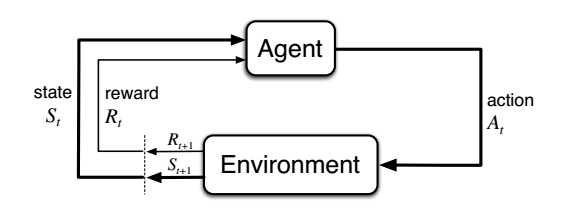
\includegraphics[width=350px,height=200px]{rl_diagram.png}
        \caption{RL}
        \label{fig:my_label}
    \end{figure}


"Reinforcement learning is learning what to do and how to map situations to actions so as to maximize a numerical reward signal" Sutton (pg 1)

A full discussion of reinforcement learning is not required to understand AlphaZero but it is necessary to look at the fundamental concepts that make up the algorithm. I present a sort hierarchy of concepts that are necessary to understand AlphaZero fully. It is possible to read through the paper or a tutorial to get the mechanics of the algorithm but to understand the "why" you will need to go deeper. 

    \begin{figure}[H]
        \centering
        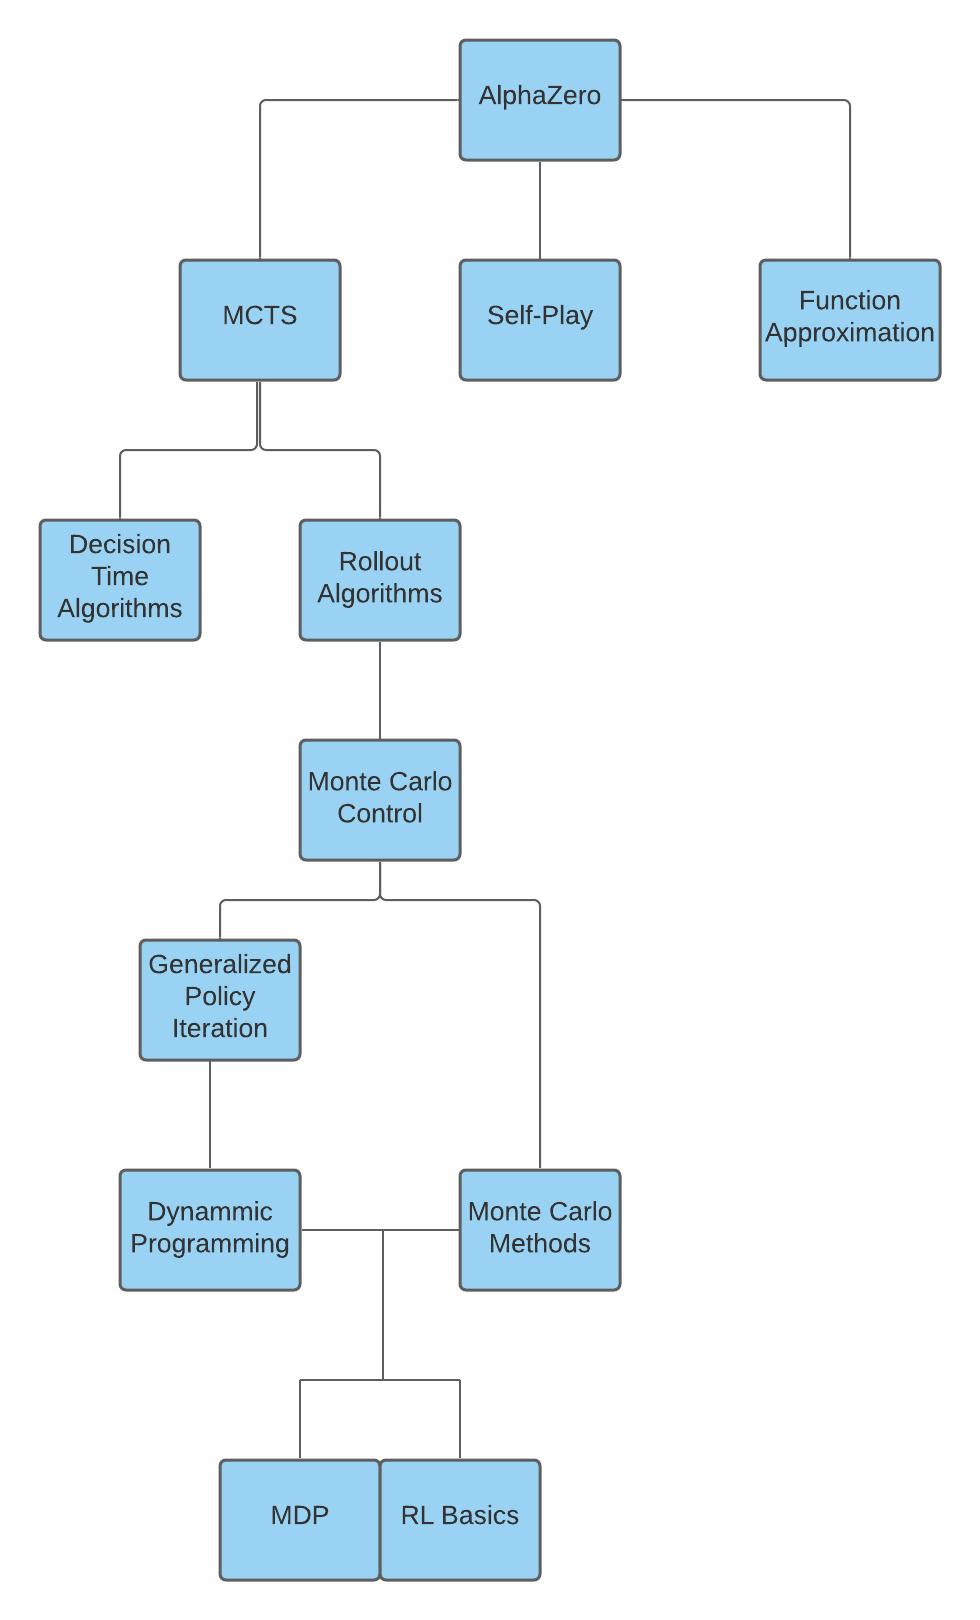
\includegraphics[width=350px,height=300px]{images/alpha_hierarchy.png}
        \caption{Concept Hierarchy}
        \label{fig:my_label}
    \end{figure}
    
    \subsection{Environment}
    
    Loosely defined as the thing that the agent interacts with. Everything that is exterior to the agent. The environment typically encompasses the system that is trying to be solved. It also provides observations and rewards as the agent takes actions. For example when trying to solve the game of Go the agent (the players) takes actions (moves pieces) and the environment is the board, the pieces, and the mechanism for telling the agent the current reward (win / loss) or other special states that are specific to the game. So it is the game itself plus a few other mechanisms to make the learning process possible. Occasionally in problems like robotics and similar problems the agents own physical body can be part of the environment. The agent will need to control its own body to achieve a task and so it will usually model its body as part of the environment in this case. The environment is not synonymous with state as observed by the agent. We will look at that next. 
    
    \subsection{State}
    
    State is the representation of all information that is available to the agent at any given time. As said above this is not necessarily the same as the observation provided by the environment. For instance in AlphaGo Zero we will see that the state is actually a function of the current board as well as previous board positions. It is up to the designer of the reinforcement learning algorithm as to what is the best state to present to an agent. In many environments the choice might be more obvious than others. 
    The fact that state is something that needs to be decided upon by the designer of the algorithm hints at a potential need for more generalization within algorithms. MuZero and similar algorithms take a step in this direction by having the agent learn that representation. MuZero as will be discussed towards the end of this paper searches in a latent space. So the state as provided by the environment is projected onto a latent space and then the algorithm searches within this space. This is an interesting approach. For further discussion on this see \cite{predictron,muzero}
    
    \subsection{Policy}
    
    A policy roughly speaking is just a definition of an agents behavior given a perceived state of the environment. That is it is a mapping $ \pi: s \rightarrow a $ where s is a state of the environment and a is an action  $ a \epsilon A $. A is the possible set of actions the agent can take. It can be either discrete or continuous. In AlphaGo Zero actions are integers representing the place on the board.
    
    \subsection{Reward Signal}
    
    A reward signal is what defines the goal of a RL algorithm. As an agent observes an environment it receives feedback in the form of rewards. Generally an agent is simply trying to maximize the sum of its reward over the long run. Rewards help the agent to learn a policy. An agent will adjust the actions that it takes based off of the feedback it receives. Roughly speaking the agent will adjust to take actions more frequently that it perceives to return more reward. In environments like AlphGo Zero there is what is called the "sparse rewards" problem. This means that the agent might be interacting with the environment for long extended periods of time before receiving any feedback. 
    
    
    \subsection{Value}
    
    The value of a state in reinforcement learning is the amount of reward an agent should expect to receive in the long run from a given state. An agent is not given this number and is something that needs to be learned. This is generally expressed like this $ V(s) \rightarrow \mathbb{R} $. 
    
    From Sutton
    $ v_{\pi}(s) = E_{\pi}[G_{t}| S_{t} = s]$
    
    
    \subsection{Model}
    
    A model from the perspective of RL typically refers to a predictive model of the environment. It is a way for the agent to predict the behavior of the environment. This allows the agent to make inferences about what will happen when certain actions are taken. This in turn allows the agent to plan based on the model. Algorithms that use models are called \textit{model-based}. Algorithms that dont explicitly model the environment are called \textit{model-free}. The line between the two can easily become blurred as a lot of algorithms will mix between the two approaches. In the context of this paper AlphaZero and can be viewed as a Model free algorithm and MuZero as a model based extension to AlphaZero. MuZero attempts to learn the dynamics of the environment from scratch whereas for AlphaZero the dynamics are known upfront.  


\section{Markov Decision Processes}

The following section draws pretty heavily from Sutton \cite{sutton}. Lets put some of the previous concepts together into a framework that we can actually use to make decisions. Markov decision processes (MDP) are an idealized environment for making sequential decisions. MDPs have been studied quite thoroughly and although their formulation is simple it is also quite robust and a surprisingly large number of problems can be formulated as MDPs. Figure 2.1 that we looked at before is an example of a MDP. What kind of data would we get if we allowed the process in that figure to go on for many time steps? First the agent begins in the start state $S_{0}$ and takes action $A_{0}$ and receives a reward $R_{1}$ and the next state $S_{1}$. Then the agent would take another action $A_{1}$ and so on. This would result in a series of data points $S_{0},A_{0},R_{1},S_{1},A_{1},R_{2},S_{2},A_{2}....R_{T},S_{T}$. Here there is some terminating condition at time $T$ but the series could also just go on continuously. $R_{t},S_{t}$ are both random variables whose probability of occurrence only depends on the previous action and reward. This is what makes the process markovian and is called the Markov property. The only thing that matters in determining the probability of the next state and reward is the current state and action. The dynamics of this process can be described by a function $p: S x R x A x S \rightarrow [0,1] $. The function can be defined in terms of conditional probability. 

$$ p(s^{'},r | s, a) = Pr\{S_{t + 1} = s^{'}, R_{t + 1} = r | S_{t} = s, A_{t} = a\}$$

So the probability given by $p$ describes the entire environment dynamics. The Markov property as described in \cite{sutton} "is best viewed as a restriction not on the decision process, but on the state. The state must include information about all aspects of the past agent–environment interaction that make a difference for the future".

How state, action and time is defined is quite flexible in this formation. Time does not have to refer to an actual interval of time but can just be some set of steps that happen one after the other. Actions likewise can really be any decision that we want to learn how to make. 

Now that we have defined the system what is the actual goal? We want to get as much reward as possible. That means no just the reward that we receive right now but all the reward we accumulate. This statement results in the \textit{reward hypothesis} {Introduction to reinforcement learning}

\say{..what we mean by goals and purposes can be well thought of as the maximization of the expected value of the cumulative sum of a received scalar signal (called reward)}.

Since learning from rewards has become so popular it might not seem like that strange of a concept and indeed it might be fairly intuitive. However this is one of the things that distinguishes reinforcement learning from other forms of machine learning. In a typical supervised learning setting for instance you attempt to minimize a loss function on a set of observed data w.r.t to some given labels. Like attempting to predict credit card fraud from a set of features. You are first given a bunch of examples with labels as to whether fraud occurred in that particular instance. You then want to train a model to be able to generalize from these observed features and labels to unlabeled or data that has not been seen yet. Reinforcement learning is different in that we dont generally start out with a set of features and labels. The agent produces data or observation as we act in the environment. Then through these observations we change the agents behavior as to achieve a desired goal. There is a bit of an art in setting up the rewards correctly. The designer of the algorithm has to choose the rewards for an environment and it is not always trivial. For GO and other two player zero sum games it is natural to assign a reward of +1 for winning, -1 for losing and 0 for a draw. You might however want to assign a small amount of reward to a draw so that the agent is receiving some amount of feedback. You might want to set up intermediate goals as to "show" the agent the right choices to make or steer them away from obviously bad choices. An example of a miss application of reward assignment would be in chess to give reward to an agent for pieces captured. This can lead the agent to commit detrimental errors to the main goal of winning just to achieve the sub goal so care must be taken that the subgoals align with the main goal. 

In this paper we will be focused on situations in which there is a clear start and end state. There are of course other domains in which this is not the case. Self-driving cars, trading in markets, and playing atari games are a few examples. Since we are trying to maximize an accumulated reward we can define our main goal as the following. 

\begin{equation}\label{Cumulative sum}
 G_{t} = \sum_{k=t + 1}^{k=T} R_{k}
\end{equation}

There is something still not quite right here. In this formulation we would value rewards at all time steps equally. This is usually not the case in most tasks however. The idea that 100\$ today is better than 100\$ 10 years from now applies here. Typically the reward we get now is more valuable then the same amount in the future. So we can modify our goal a bit by discounting rewards that we receive farther into the future. We do this by using a discount factor $\gamma < 1$. 

\begin{equation}\label{Discounted Cumulative Sum}
G_{t} = \sum_{k=t + 1}^{k=T} \gamma^{k - t + 1} R_{k}
\end{equation}

Ok, great we have a goal now how do we use that goal to start defining how the agent is going to behave? Well we want the agent to take actions that are going to lead to higher $G$. Taking actions in our MDP formulation leads us to end up in different future states. So we want to end up in better states. What does it mean to be a better state? A better state is one that leads to more $G$. So we want to be in states in which we expect to collect more reward in the future. Lets try and put this into something concrete. The expected value of a state seems to fit well into what we are going after so we can use that as a starting point. 

\begin{equation}\label{Expected State Value}
\mathbf{v}_{\pi}(s) \dot{=} \mathbb{E}_{\pi}[G_{t} | S_{t} = s]
\end{equation}

The $\pi$ here refers to the policy of the agent. So this is looking at the expected value assuming the agent is following a given policy. We discussed policies previously and we will discuss them more in the future. It is important for knowing the expected value while following an MDP because a policy will define how we transition from one state to the next. We can also define a value function for a state action pair in a similar manner. 

\begin{equation}\label{Expected State Action Value}
\mathbf{q}_{\pi}(s,a) \dot{=} \mathbb{E}_{\pi}[G_{t} | S_{t} = s, A_{t} = a] 
\end{equation}

Its quite easy to see that if one actually had access to one of these functions how you might have the agent behave. In the case of $\mathbf{q}_{\pi}$ simply pick the action with the largest value. We of course don't have access to these and have to learn them from experience. How might we do this? One way is to somehow track the average return that you get from a particular state or state action pair. This approach is called Monte Carlo methods. This is quite relevant for understanding AlphaZero as a form of tree search called Monte Carlo tree search is central to the algorithm. 
    
One central idea in reinforcement learning is the ability to view a value function recursively. Lets look at how we can do that. First we can write our cumulative variable $G_{t}$ in terms of the next immediate reward and a discounted cumulative return starting from the next timestep.  

    $$ \mathbb{E}_{\pi}[G_{t} | S_{t} = s] = \mathbb{E}_{\pi}[R_{t + 1} + \gamma G_{t + 1} | S_{t} = s] $$
    
Then we can expand this by thinking about what en expectation means here in terms of our random variable $R_{t + 1}$. In words it is the value of all future rewards we would see by transitioning to new states. We have said previously that the probability of transitioning to a new state $s^{'}$ and receiving reward $r$ from the current state given a certain action is given by the function $p(s^{'},r|,s,a)$ the system dynamics of our MDP. We know the definition of expected value is the sum over possible outcomes of a random weighted by the probability of that outcome happening. So we can write the expected value of $R_{t}$ given a specific state and action. 

$$ \mathbb{E}[R_{t} | S_{t} = s] = \underset{s^{'},r}{\sum}p(s^{'},r|,s,a)[ r ]$$

We want however to look at the expectation following a specific policy. A policy $\pi(a|s)$ gives us a distribution over possible next actions given the current state. So we can further expand on our previous equation. 

$$ \mathbb{E_{\pi}}[R_{t} | S_{t} = s] = \underset{a}{\sum}\pi(a|s)\underset{s^{'},r}{\sum}p(s^{'},r|,s,a)[ r ]$$

We can now go back to our expectation of the cumulative reward. 

$$\mathbb{E}_{\pi}[R_{t + 1} + \gamma G_{t + 1} | S_{t} = s] = \underset{a}{\sum}\pi(a|s)\underset{s^{'},r}{\sum}p(s^{'},r|,s,a)[ r + \gamma \mathbb{E}_{\pi}[G_{t + 1} | S_{t + 1} = s^{'}]] $$

Notice how the expectation is now conditioned on the next state. This allows us to rewrite this in a recursive form.

\begin{equation}\label{Bellman State Value Equation}
\mathbf{v_{\pi}(s)} = \underset{a}{\sum}\pi(a|s)\underset{s^{'},r}{\sum}p(s^{'},r|,s,a)[ r + \gamma \mathbf{v_{\pi}(s^{'})}]
\end{equation}

This last form is know as the bellman equation. The bellman equation represents values of a state in terms of values of future states. The figure below taken from Sutton represents this as a decision tree. The open circles are states and the black circles are actions. This shows if you are in state $s$ you have 3 actions that are part of policy $\pi$. Once you take one of those actions the environment then transitions to one of two next states $s^{'}$ and emits a reward $r$ with probability $p$. You could then extend the diagram in the same way from each of the next states. If this were a two player game the other player would be part of the environment and the probability of transition to state $s^{'}$ would depend on the other players policy $\pi$. Sutton refers to these as backup diagrams because they show how information could be propagated back up the tree. 

\begin{figure}[H]
        \centering
        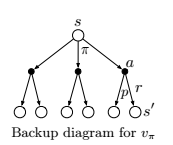
\includegraphics[width=350px,height=200px]{images/bellman_update.png}
        \caption{RL}
        \label{fig:my_label}
\end{figure}

\section{Tictactoe Bellman Equation}

Lets try and picture what the bellman equation might look like for the game of tictactoe. This example will help to both illustrate how the equation works and also the intractability of calculating it in practice. The figure below shows the initial blank board at the beginning of the game. To calculate the value of this position we will do so from player X's perspective. There are nine possible next moves and so each of those needs to be assigned a probability represented by the policy $\pi(a | s_{0})$. Then focusing on action $a_{0}$ at the top of the diagram the next thing we would need to do would be to calculate $p(s^{'},r|,s,a)[ r + \gamma \mathbf{v_{\pi}(s^{'})}]$ for each of the possible next states. So we could start with $p(s_{1},r|,s_{0},a_{0})$. What is this probability? We will need to know this beforehand. How it is obtained depends. We might just be given the distribution beforehand as part of our model of the environment. In this instance however a more intuitive candidate would be to ask player "O" for their policy. That is if we had access to $\pi$ from player "O" perspective that would be then give the associated probability of future states since future states are just the board after "O" has chosen an action. Now that we have $p(s_{1},r|,s_{0},a_{0})$ we need $[r + \gamma v(s_{1})]$. The reward $r$ here refers to the immediate reward observed. In the case of tictactoe and most other two player board games there will be no reward till the end of the game. So $r$ here is just 0. So we need $\gamma v(s_{1})$. Here $\gamma$ is a discount factor and is constant and chosen beforehand. The $v(s_{1})$ calculation is shown next. 

\begin{figure}[H]
        \centering
        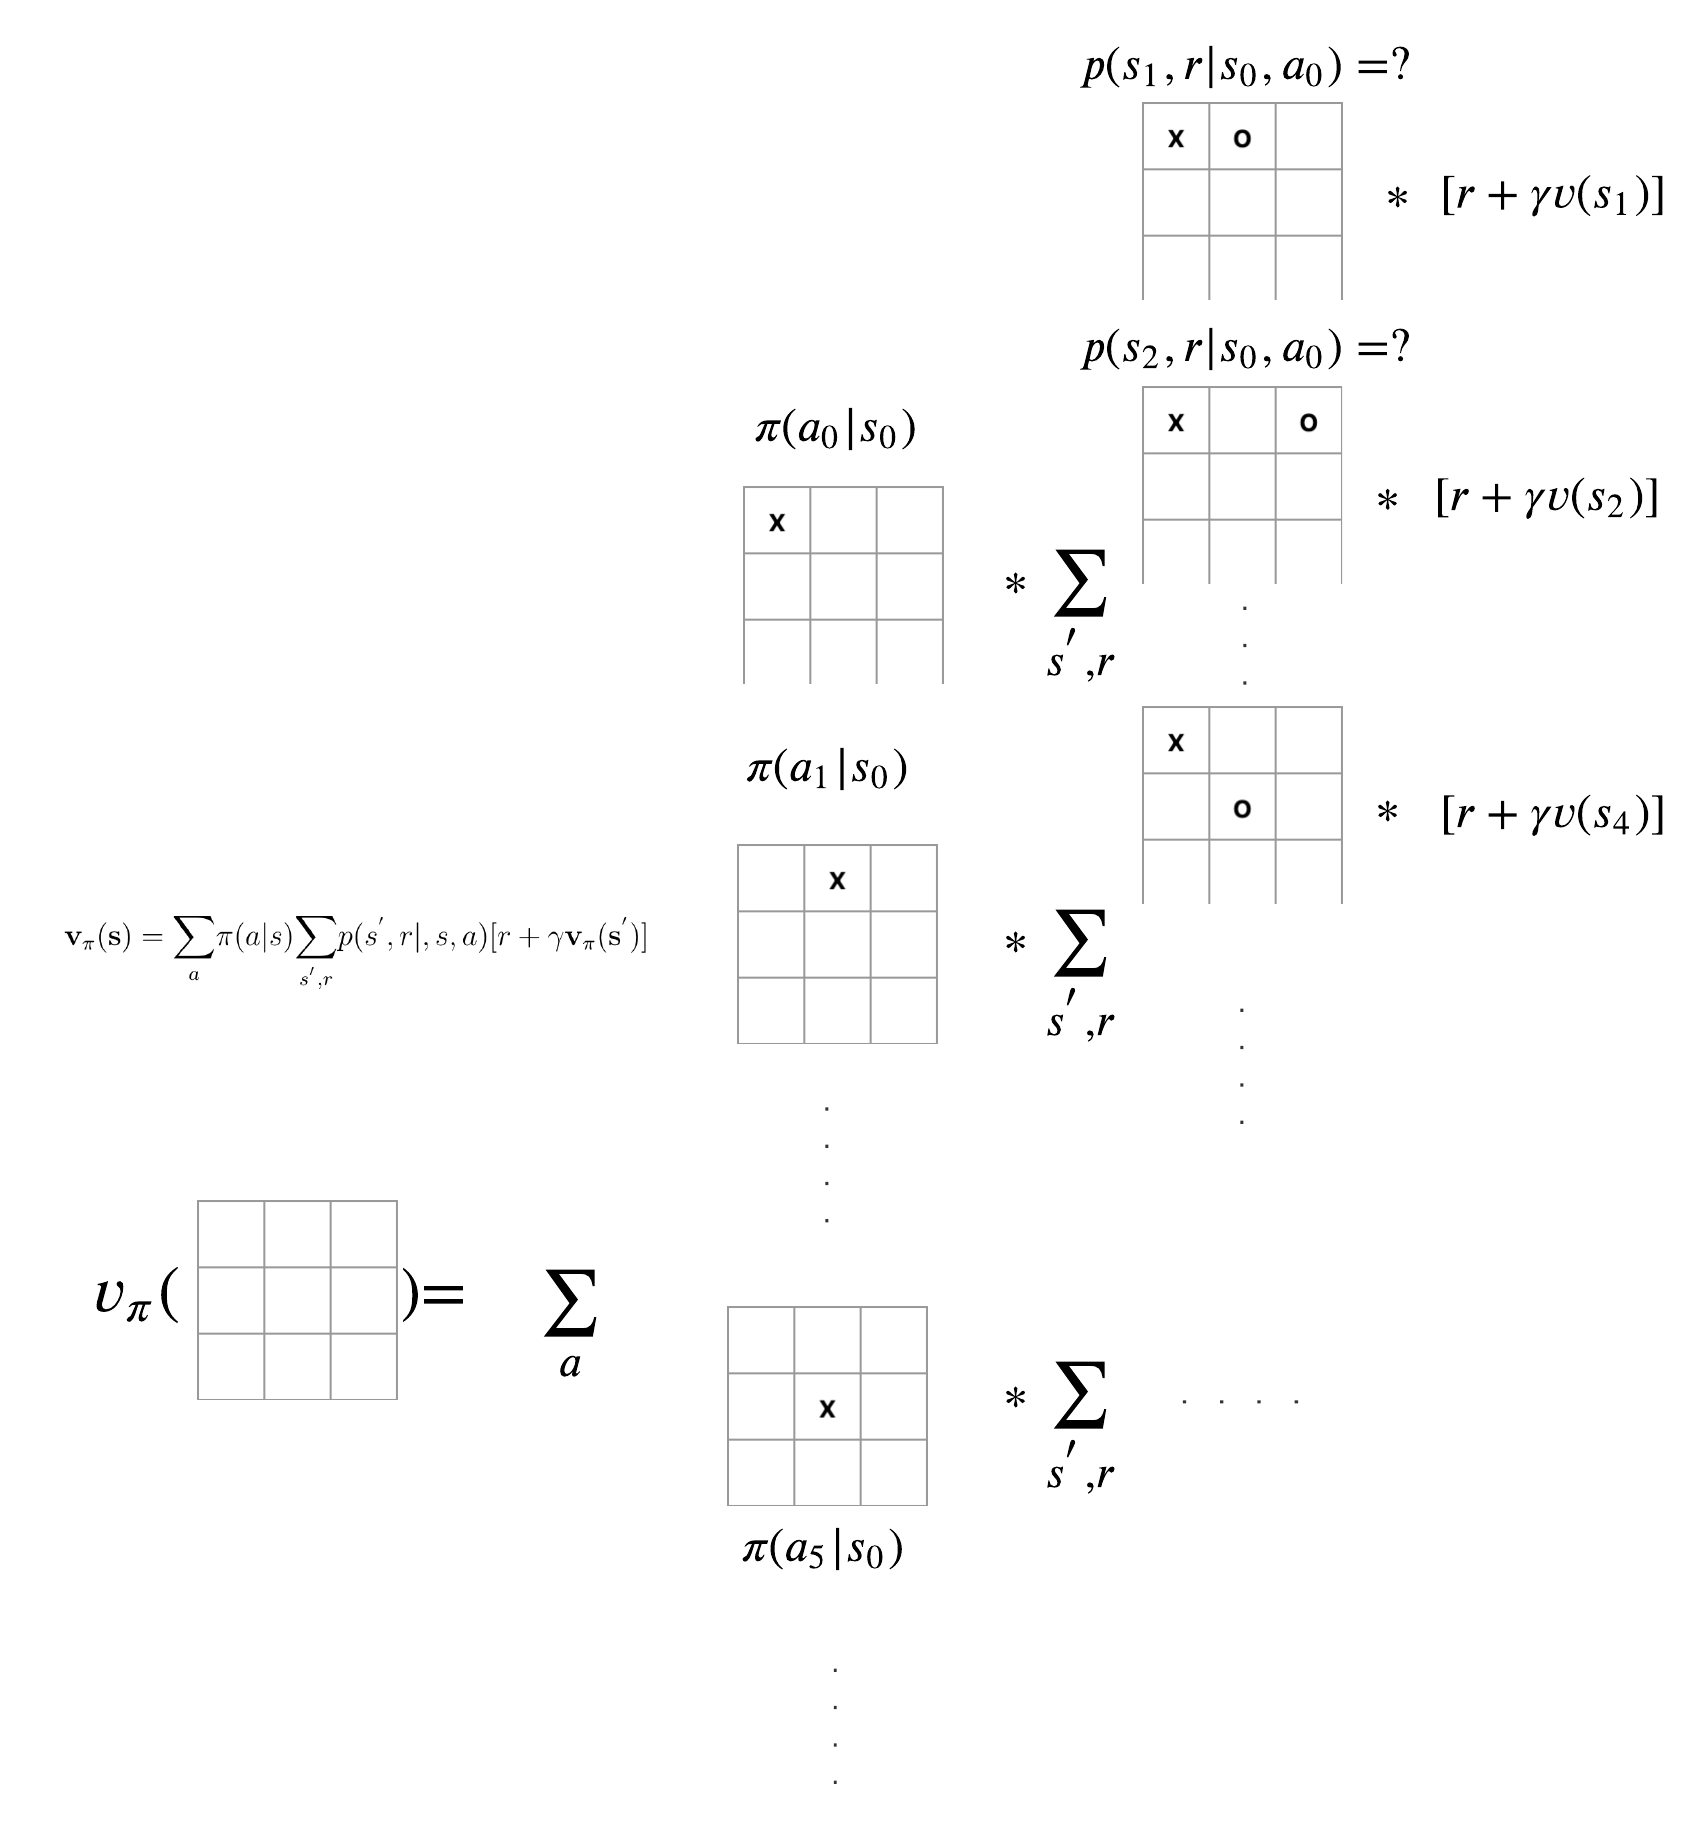
\includegraphics[width=400px,height=300px]{images/PolicyEvaluationExample/intractable_value_function.png}
        \caption{Tictactoe Bellman 1}
        \label{fig:tictactoe-dp}
\end{figure}

In figure 2.5 below we see the same calculation expanded out but for state $s_{1}$. This same sort of recursive procedure would keep going until a terminal state was reached. For tictactoe this occurs only when the game ends and a reward of 1,-1 or 0 is assigned for win,loss or draw. 

\begin{figure}[H]
        \centering
        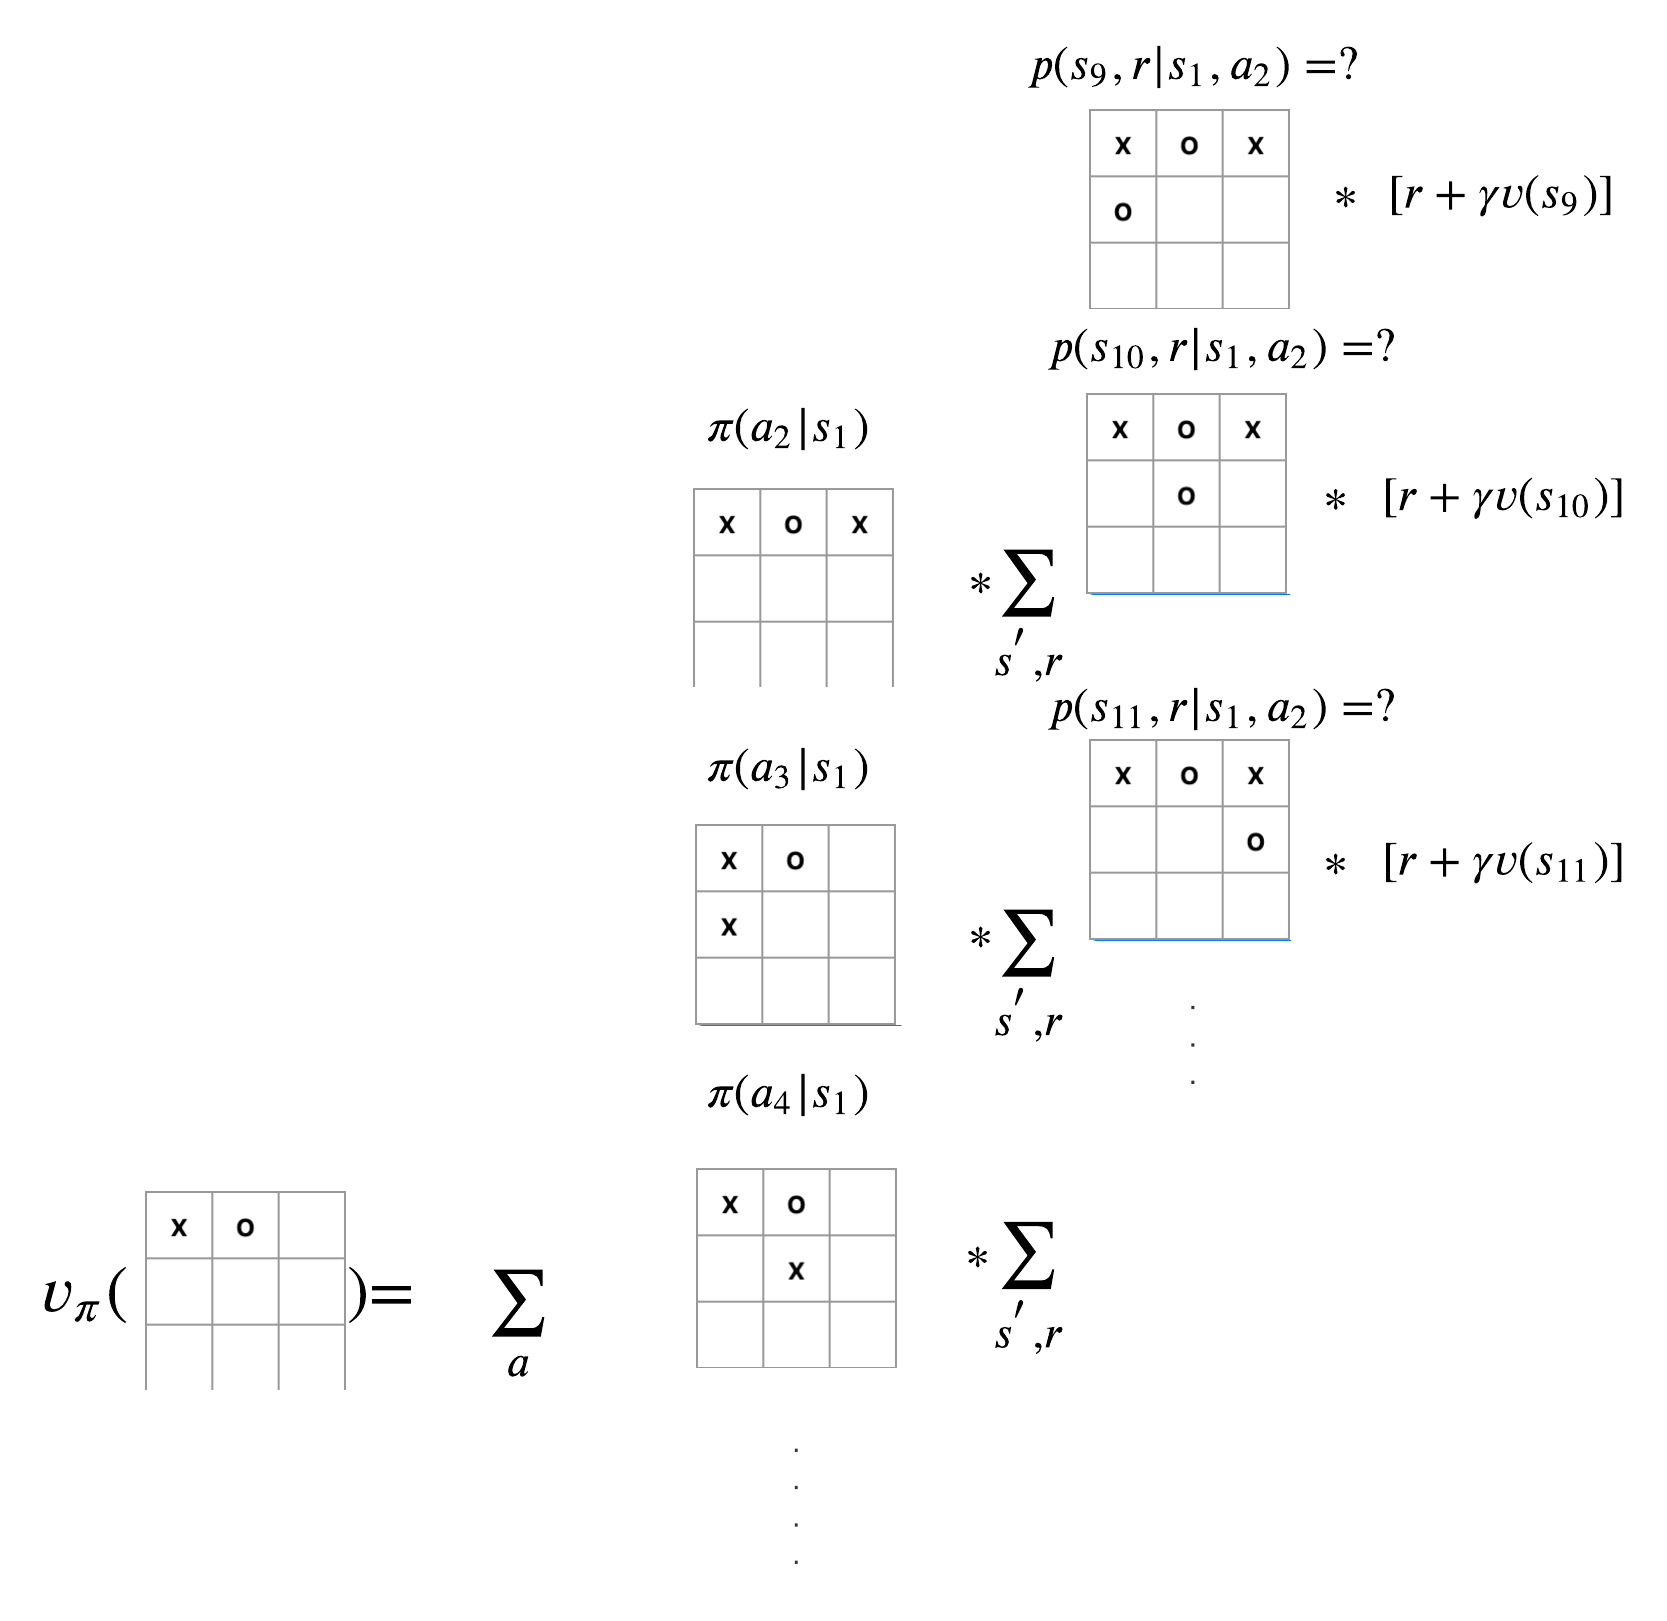
\includegraphics[width=400px,height=300px]{images/PolicyEvaluationExample/intractable_value_function_2.png}
        \caption{Ticatactoe Bellman 2}
        \label{fig:my_label}
\end{figure}

\section{Policy evaluation Example}

Lets look at an example of evaluating this a value function for a specific state and policy using a more simple tictactoe example as a test case. Consider the board below. It is player X to go. How to you calculate equation (2.5)? Once again we need access to a policy and access to the transition probability distribution. 

\begin{figure}[H]
        \centering
        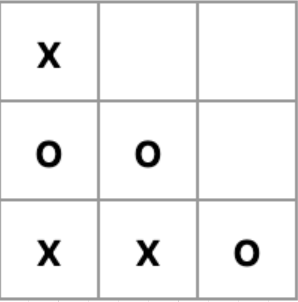
\includegraphics[width=150px,height=150px]{images/PolicyEvaluationExample/pe_example_s0.png}
        \caption{policy eval 1}
        \label{fig:my_label}
\end{figure}

Lets ignore that this is a two player game for a moment. From player X's perspective all we need is to set our own policy. Then the next state we observe after taking an action will be given by the environment. In this case player "O" will just be part of the environment. The situation is displayed in the figure below. We have three possible actions to take. We can see what the correct thing to do is but a computer has no idea! So lets assign probability $\frac{1}{4}$ to the top two actions and $\frac{1}{2}$ to the other action. When the agent takes action $a_{2}$ or the top right square he observes a next state $s_{1}$ and reward $-1$. This event happens with probability one and so no other events occur after taking that action. The same is shown for action $a_{1}$. For action $a_{5}$ the next state is observed but it is not a terminal state so a policy needs to be defined. There is only one action so the definition is simple. No next state is observed just a reward of 0 since it is a terminal state. Lets now actually calculate $v_{\pi}(s_{0})$ 

\begin{figure}[H]
        \centering
        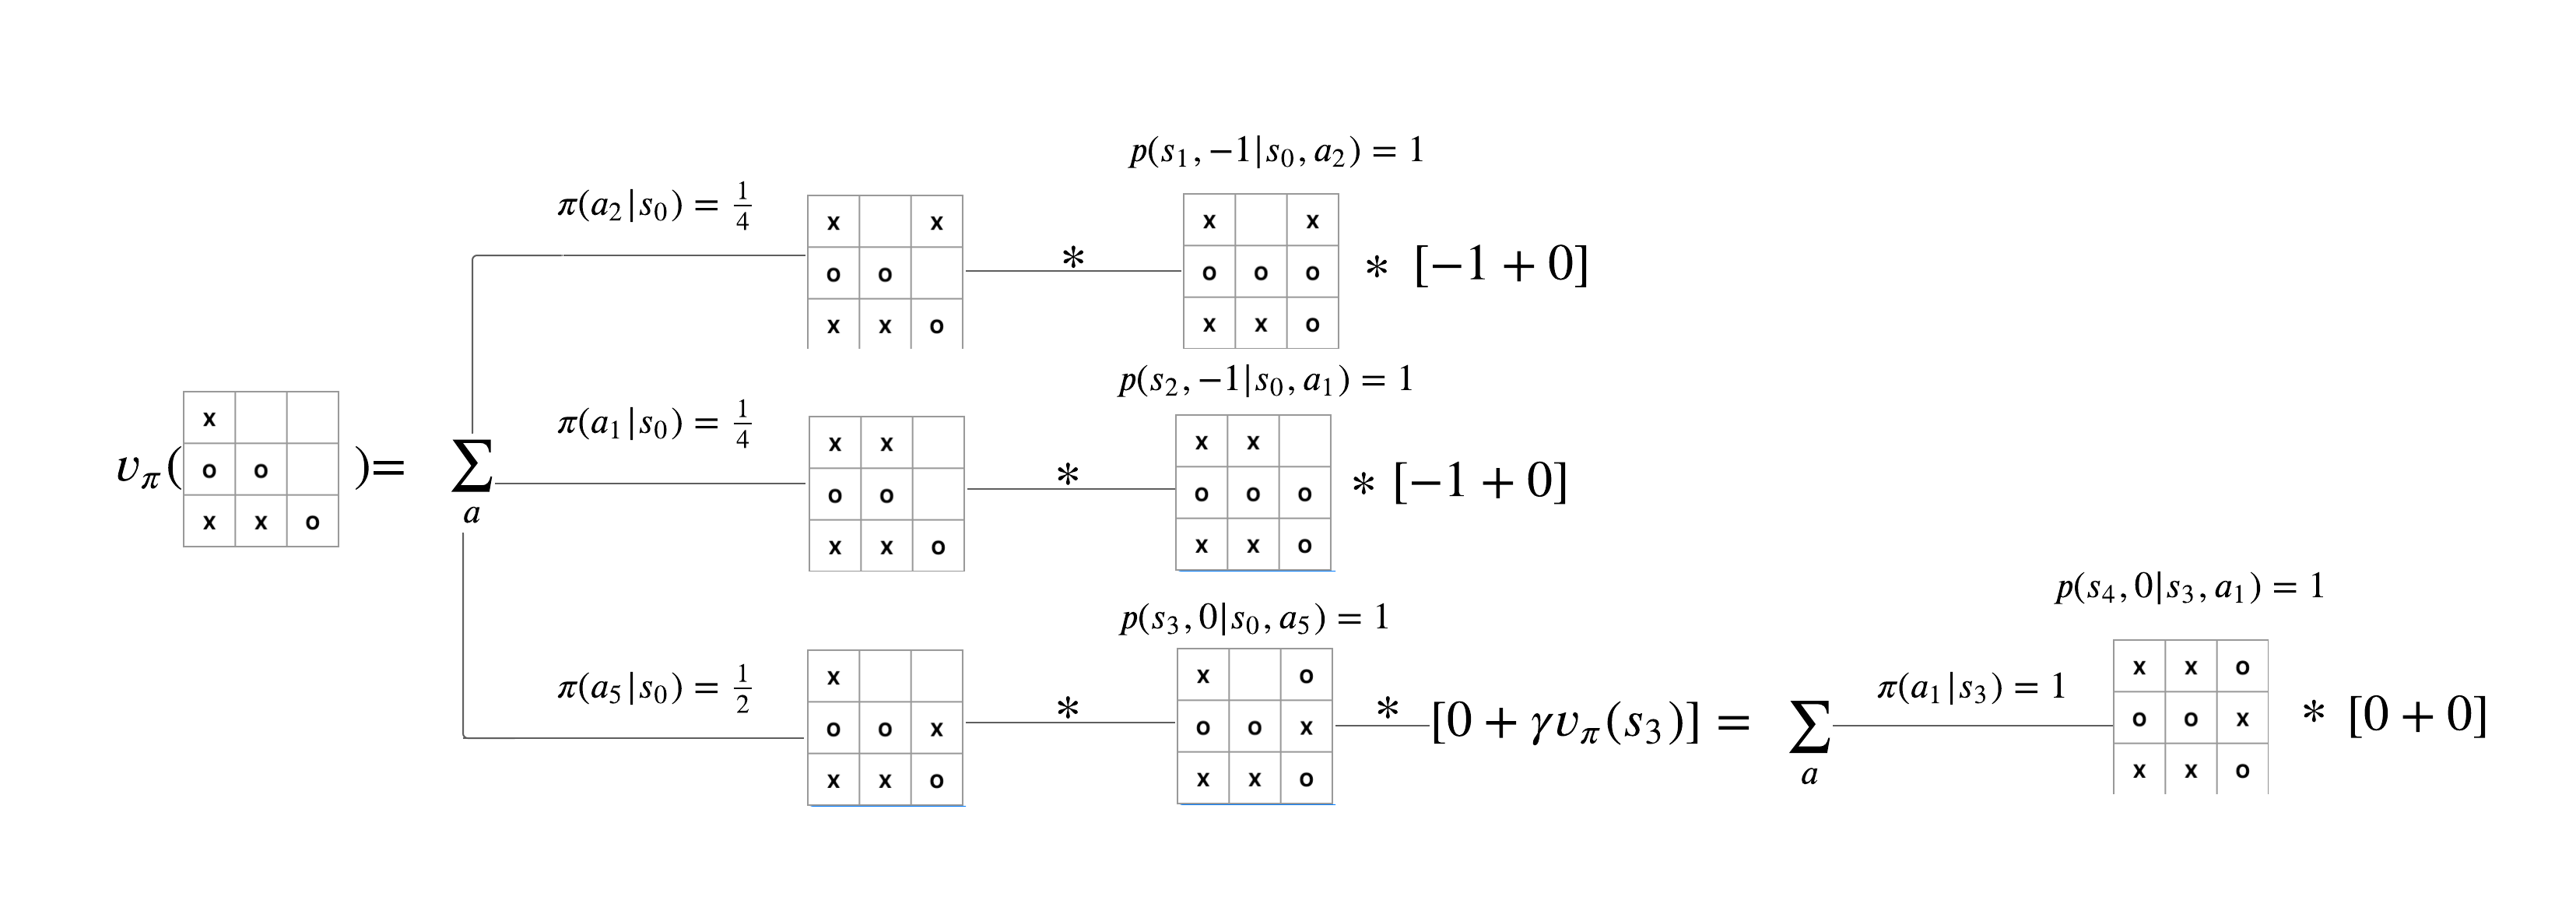
\includegraphics[width=400px,height=250px]{images/PolicyEvaluationExample/value_function.png}
        \caption{policy eval 2}
        \label{fig:my_label}
\end{figure}

Lets calculate the value of using this policy from the initial state using equation (2.5). With the small number of states being used this is a fairly easy calculation but its easy to see how this could easily start to become intractable. 

\begin{figure}[H]
        \centering
        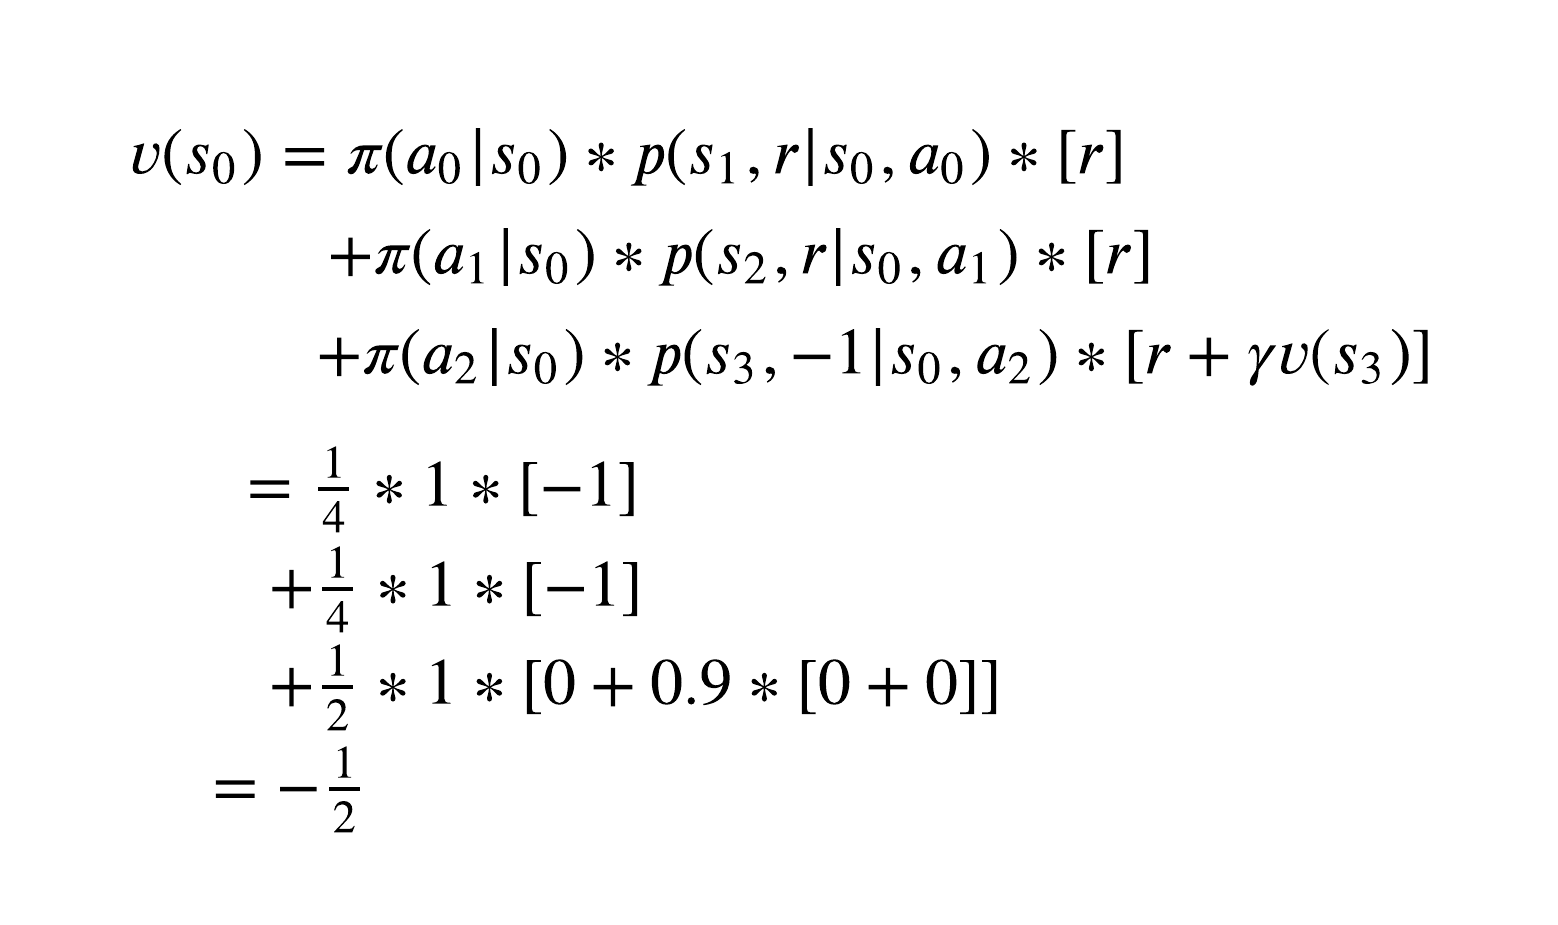
\includegraphics[width=400px,height=200px]{images/PolicyEvaluationExample/value_function_calc.png}
        \caption{policy eval 3}
        \label{fig:my_label}
\end{figure}

We have now discussed how to evaluate given states within our framework. We have not discussed yet how to actually use this information to make good decisions. There is a theorem in RL that says that a policy $\pi$ is better than or equal to another policy $\pi^{'}$ if its expected value is greater than or equal to the expected value of $\pi^{'}$ for all states. In other words $ \pi \geq \pi^{'} $ iff $ \mathbf{v_{\pi}}(s) >= \mathbf{v_{\pi^{'}}}(s)$ for all $ s \in  S$. It has also been shown and we will restate here without proof that an optimal policy always exists for an MDP. There can be more than one but at least one exists. The notation used for the optimal policy is usually $\pi_{*}$ and we will take that notation here as well. This leads also to the fact that there is an optimal state value function. 

\begin{equation}\label{Optimal State Value Equation}
\mathbf{v_{*}}(s) \dot{=} \underset{\pi}{max} \: \mathbf{v_{\pi}}(s) , \: \forall s \in S 
\end{equation}

The bellman equation representation must hold as well. In our previous representation of the bellman equation we had to sum over all actions from our policy $\pi(a |s)$. When looking at an optimal policy in the case of an MDP we will only be interested in taking the best action. So we can rewrite the bellman equation of the value function with that in mind. 

\begin{equation}\label{Optimal Bellman State Value Equation}
\mathbf{v_{*}}(s)= \underset{a}{max}\underset{s^{'},r}{\sum}p(s^{'},r|,s,a)[ r + \gamma \mathbf{v_{*}(s^{'})}]
\end{equation}


A similar analysis can be done for $q(s,a)$. We will not go through that here but you can look to Sutton or other sources for more discussion. We will simply present the result here. 

\begin{equation}\label{Optimal Bellman State Action Value Equation}
\mathbf{q_{*}}(s,a)= \underset{s^{'},r}{\sum}p(s^{'},r|,s,a)[ r + \underset{a}{max} \: \mathbf{q_{*}}(s^{'},a^{'})]
\end{equation}

I think that the $\mathbf{q_{*}}$ optimal value function can be more intuitive. It simply says that the value of the optimal action from the current state is a weighted sum over possible next states assuming we take the optimal action from those states as well. If you have $\mathbf{q_{*}}$ or $\mathbf{v_{*}}$ than coming up with the correct policy is easy. For $\mathbf{v_{*}}$ you just have to do one step look ahead to see which actions will give you the max. You dont have to continue to look further because you already have access to the optimal values of the next state. With $\mathbf{q_{*}}$ you simply look up the best action from the current state. No further search is necessary. Obtaining these optimal functions of course generally takes a lot of work and in any large setting is intractable to compute directly. To actually compute an optimal bellman equation you need to have perfect knowledge of the environment, sufficient resources and the markov property. These assumptions typically dont hold for most interesting problems. For any problem that breaks one of these assumptions some sort of approximation will be needed. One approach that fits in closely with the bellman optimality equation is dynammic programming which we will discuss shortly. One big takeaway from reading Sutton and others work is that most reinforcement learning techniques come down to different ways of approximating the bellman optimality equation. To me this is quite powerful and means that even though we might come across some powerful approximation techniques such as those that we see in AlphaZero they can all be viewed from the perspective of approximating the bellman equation in some way. 

\section{Dynamic Programming}

Dynamic programming (DP) is one of the more foundational topics within reinforcement learning. We will not dwell on this topic too long but there are a few important lessons in which DP can help inform our understanding of RL and AlphaZero. We have just concluded discussing optimal value functions and now we need to find a way to actually compute them. That is where DP comes in. DP is essentially a collection of algorithms used to compute optimal value functions. Recall that (\ref{Bellman State Value Equation}) gave us a way to evaluate the value of state given a certain policy. This equation actually gives us a system of linear equations and can be solved directly if the model of the environment is totally known. We have $|S|$ equations and $|S|$ unknowns. This of course is not computationally very feasible so we need to find a way to compute (\ref{Bellman State Value Equation}) iteratively. We can actually just turn it into an update rule like the following. 

\begin{equation}\label{Bellman State Value Update Equation}
\mathbf{v_{k + 1}(s)} = \underset{a}{\sum}\pi(a|s)\underset{s^{'},r}{\sum}p(s^{'},r|,s,a)[ r + \gamma \mathbf{v_{k}(s^{'})}]
\end{equation}

We can first initialize $v_{0}(s)$ for each state randomly. We can use domain knowledge to set reasonable initial values as well or just set everything to 0 to start. This iterative process will converge to $v_{\pi}$ as $ k \rightarrow \infty$. This is called \textit{iterative policy evaluation} and it gives us a way to evaluate the current policy $\pi$ in an iterative fashion. We of course dont have to wait for $ k \rightarrow \infty$. In practice we can implement some stopping condition for which we are satisfied that $v_{k}$ is close enough to $v_{\pi}$. 

We dont want to just know the value of a given policy however we want to find what the best policy is. So we need to find a way to update our policy as well. I will state here what is known as the \textit{policy improvement theorem}. 

\newtheorem{remark}{Policy Improvement Theorem}

\begin{remark}\label{Policy Improvement Theorem}
Let $\pi$ and $\pi^{'}$ be any two separate deterministic policies for all $s \in S$ s.t. $q_{\pi}(s,\pi^{'}(a)) \geq v_{\pi}(s)$. Then the policy $\pi^{'}$ is greater than or equal to $\pi$. This implies that $ \forall s \in S$ each state value function has the relationship that $v_{\pi^{'}}(s) \geq v_{\pi}(s)$
\end{remark}

The idea here is that if you can take a policy $\pi$ and change one of its actions at a particular state to guarantee that it is at least as good or better than $\pi$ at that state then you can just change the policy at that particular state to the new action and you now have a better policy $\pi^{'}$. How can we do this at every state to give us a general methodology? We can do whats called acting greedily. Acting greedily means that from a given state you take the action that maximizes return from a one step look ahead perspective according to $v_{\pi}$. We can adjust (\ref{Bellman State Value Equation}) once again to represent this. 

\begin{equation}\label{Greedy Policy}
\mathbf{\pi^{'}} = \underset{a}{argmax}\underset{a}{\sum}\pi(a|s)\underset{s^{'},r}{\sum}p(s^{'},r|,s,a)[ r + \gamma \mathbf{v_{\pi}(s^{'})}] = \underset{a}{argmax} \: \mathbf{q_{\pi}(s,a)}
\end{equation}

This just says what we have already said in words. We use the current policy $\pi$ and take the action that is going to maximize our policy evaluation from a given state using $\pi$. This gives us a new policy $\pi^{'}$ that we know from the policy improvement theorem will guarantee us an improved policy. The only way its not an improvement once again is if we already had an optimal policy. Now that we have a new policy $\pi^{'}$ how can we continue to improve it. We need to evaluate $\mathbf{v_{\pi'}}$ using policy evaluation. Then we can use (\ref{Greedy Policy}) again to get a new policy $\pi^{''}$

$$ \mathbf{\pi^{''}} = \underset{a}{argmax}\underset{a}{\sum}\pi^{'}(a|s)\underset{s^{'},r}{\sum}p(s^{'},r|,s,a)[ r + \gamma \mathbf{v_{\pi^{'}}(s^{'})}]
$$

We can then repeat this process until convergence. This algorithm is called \textit{}{policy iteration} and is given in full below. 

 \begin{figure}[H]
        \centering
        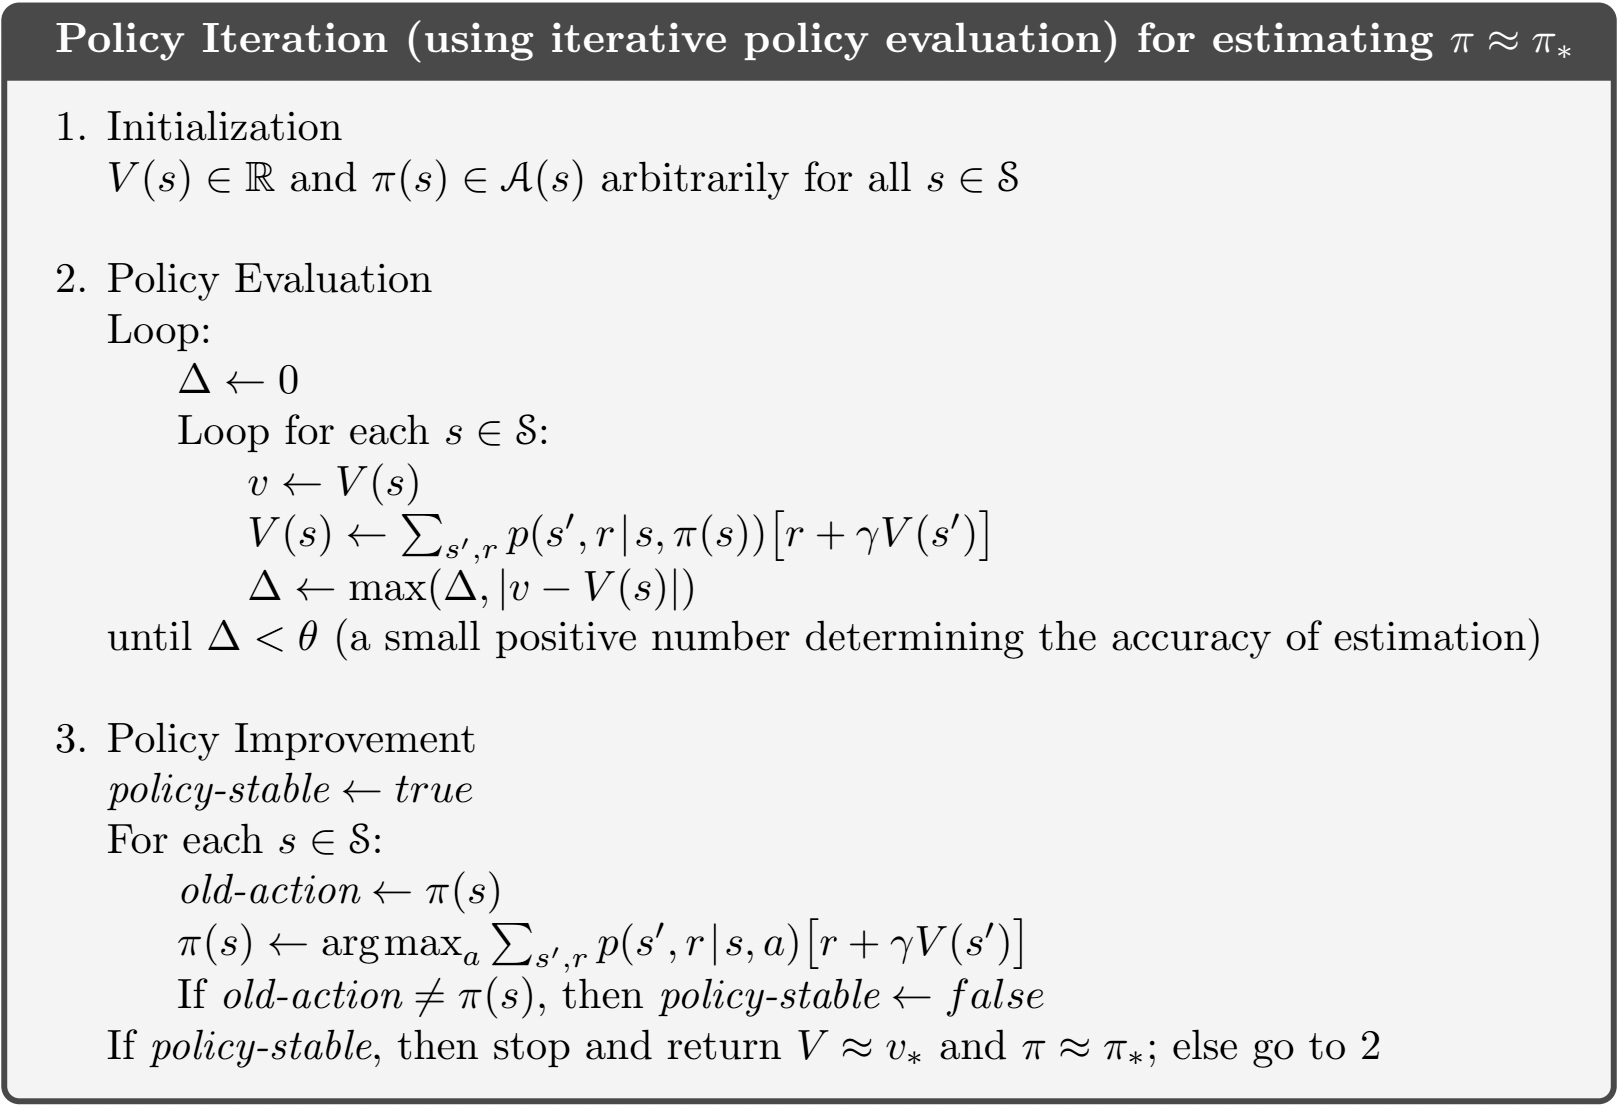
\includegraphics[width=350px,height=200px]{images/policy_iteration.png}
        \caption{From Sutton Chpt 4.3}
        \label{fig:my_label}
    \end{figure}

This idea of iterating back and forth between evaluation of a policy and improving a policy is a fairly general concept. In fact there is something called \textit{General policy iteration} (GPI) which captures these two concepts. Many reinforcement learning algorithms can be described in terms of GPI. The process is quite interesting because as soon as you perform policy improvement your value function is no longer accurate because it is still in reference to the old policy. So then you update the value function with the new policy to make it accurate again. The policy however is no longer optimal w.r.t the current value function so you adjust the policy by once again acting greedily. This goes back and forth until convergence is reached. There is a constant pushing and pulling between policy evaluation and policy improvement. 



\section{Monte Carlo Methods}

Monte Carlo in regards to reinforcement learning is a bit more specific than its typical meaning. In this discussion by "Monte Carlo" we mean any method that uses an average return for estimation. We will focus on estimating the value $\mathbf{v}_{\pi}(s)$ of a particular state. We said that our goal with $\mathbf{v}_{\pi}$ was to compute the expected value of the cumulative returns from a particular state. To apply monte carlo methods to this problem we can just track the average return we observe when visiting that particular state. We can do this directly from experience assuming the agent is following the policy $\pi$ and in the limit we should have a true estimate of $v_{\pi}$. This is called Monte carlo prediction and the most common form is called first-visit. This means that we simply average the return from the first visit to a particular state. For every visit we average the return following every visit. The first-visit method  has better understood theoretic properties. Every-visit however extends more naturally to function approximation. They both however converge to $\mathbf{v}_{\pi}(s)$ as the number of visits goes to infinity. The outline of the algorithm taken from Sutton is displayed below. 

\begin{figure}[H]
        \centering
        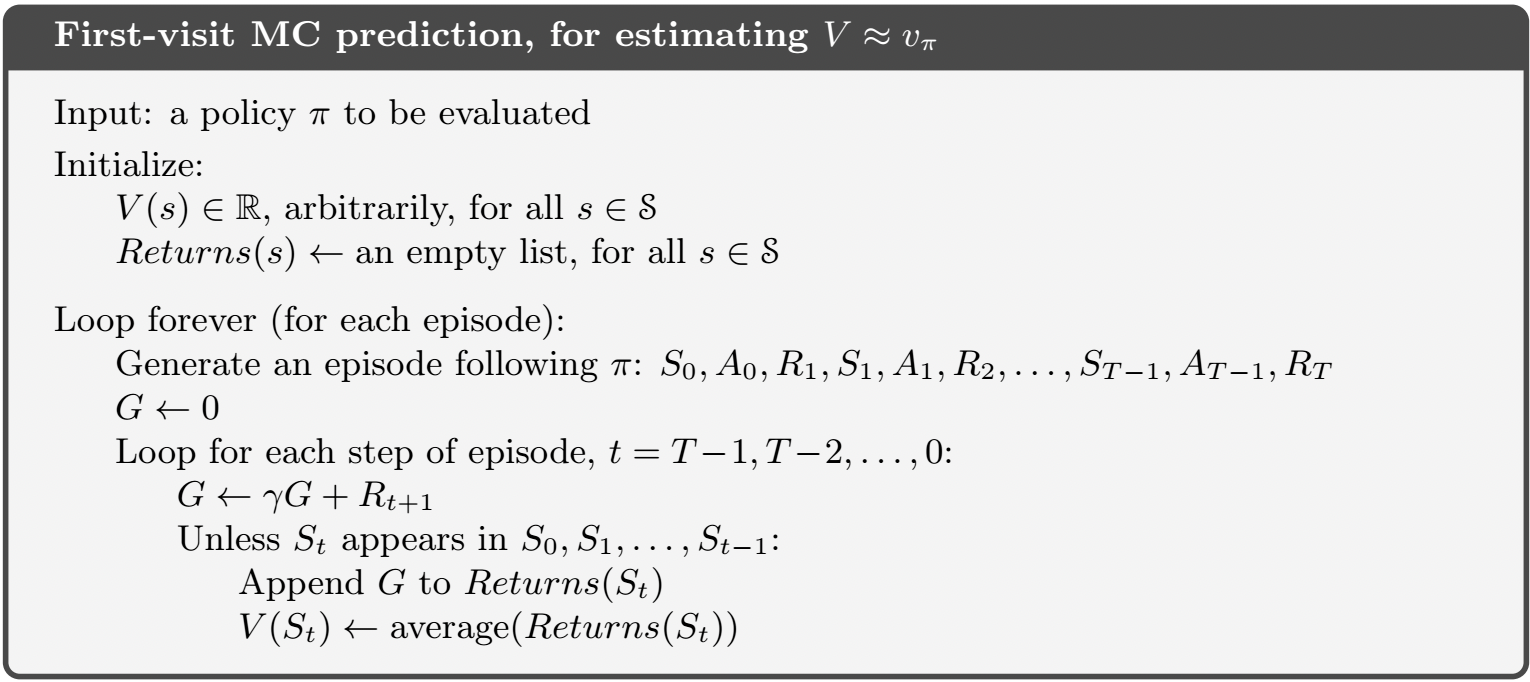
\includegraphics[width=350px,height=200px]{images/first-visit-mc.png}
        \caption{First-visit MC prediction}
        \label{fig:my_label}
    \end{figure}

Some important facts about MC methods

\begin{enumerate}
    \item One advantage of MC prediction is that we dont need to have a complete model of the environment in order to come up with an estimate for the state $s$. Since Monte Carlo Methods work with sample episodes they simply can use a given policy to keep generating samples.
    \item MC methods always run to the end of an episode whereas DP only looks one step ahead. 
    \item The estimate for each state is independent. For DP this is not the case because DP bootstraps
    \item Computational expense of estimating the value of a state is independent of the number of states
\end{enumerate}

Advantages over DP

\begin{itemize}
    \item Can learn from actual experience
    \item Can learn from simulated experience
    \item Can generate sample episodes starting from some state that your interested in and just average return from only that state and ignore the rest. 
\end{itemize}
 
Just like we saw with DP we can move from simply evaluating a given policy to actually attempting to find a best policy. We say that General policy iteration (GPI) was a flexible way of framing the problem. We can do a similar thing with MC methods. Just as before we can improve the policy by simply acting greedily w.r.t the value function $q(s,a)$. It is easier to frame a GPI model for MC methods in terms of the action-value function $q_{\pi}$ instead of $v_{\pi}$ which requires us to do a lookahead search.  So the greedy policy is defined as 


\begin{equation}\label{MC Greedy}
\pi(s) \dot{=}\underset{a}{argmax} \: q(s,a)
\end{equation}

The policy improvement theorem as discussed before applies to $\pi_{k}$ the $kth$ step of the algorithm. This means that if at each iteration of the algorithm we improve our policy by acting greedily than we can assume that the following is true. 

$$
q_{\pi_{k}}(s,\pi_{k + 1}(s)) \geq \mathbf{v}_{\pi_{k}}(s)
$$

There are two assumptions here that are necessary for convergence. The first is that sufficient exploration is happening. That is that each state action pair has some non zero probability of occurring. The second is that we need an in order to evaluate a given policy we need an infinite number of episodes. The Monte Carlo Exploring Starts algorithm is an example of one that drops the second requirement but satisfies the first by randomly choosing a state action pair to start at. The value function $Q(S_{t},A_{t})$ is able to converge accumulating and averaging returns for all episodes. Convergence although intuitively seems guaranteed has not so far been proven. The exploring starts assumption can be dropped by doing things like using a $\epsilon$-greedy algorithm that with probability $\epsilon$ takes a random action. This will ensure that all state action pairs are visited in the limit and allows you to start each episode in a more "natural" manner.

\begin{figure}[h!]
        \centering
        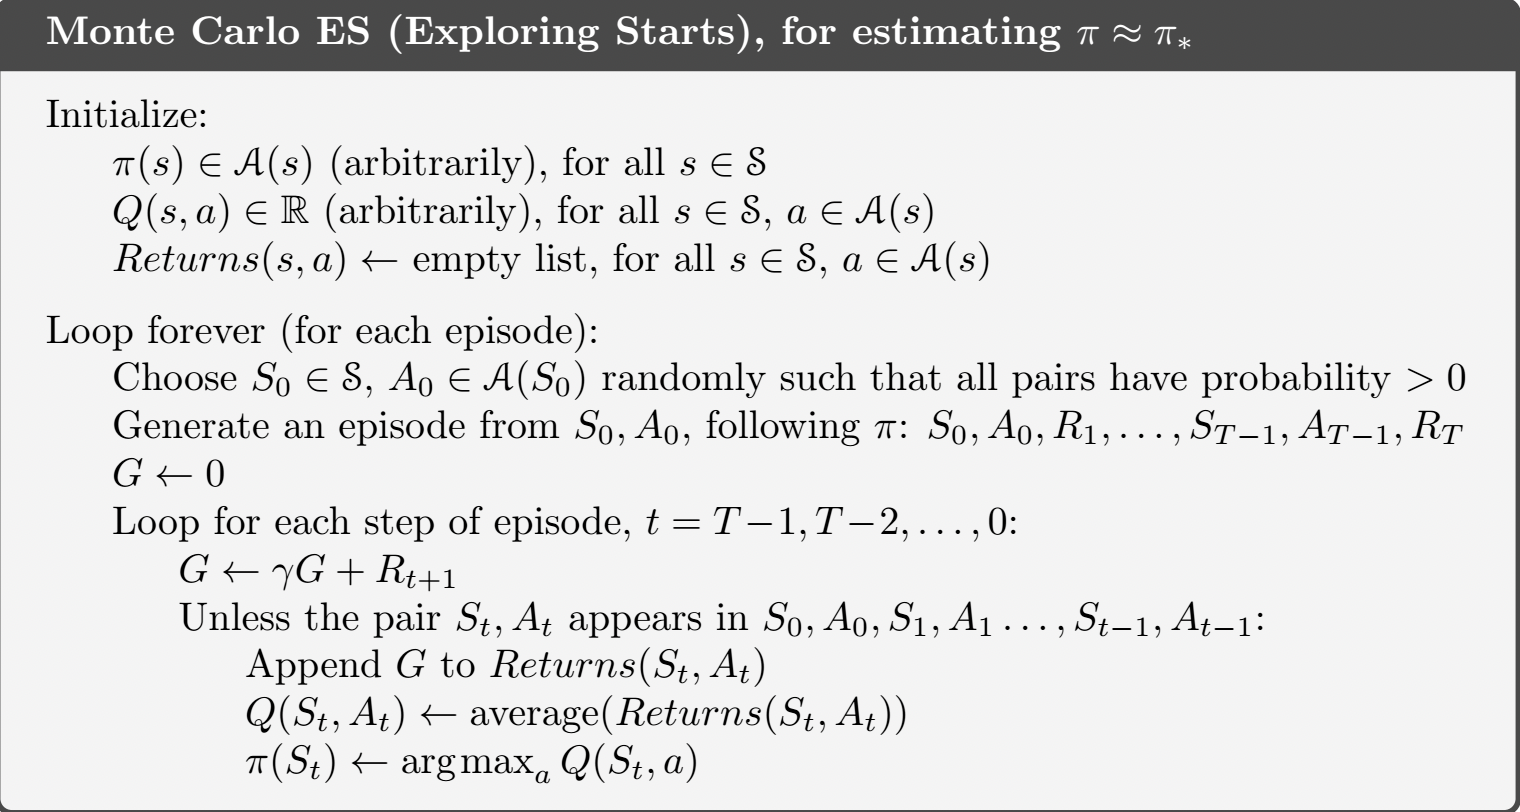
\includegraphics[width=350px,height=200px]{images/mc_es.png}
        \caption{Monte Carlo ES (Exploring Starts)}
        \label{fig:my_label}
    \end{figure}


\section{TD learning}

Temporal difference learning (TD) is an important concept in reinforcement learning and it combines a lot of the information that we have covered so far. It takes ideas from MC methods and dynamic programming. It can learn from experience like we saw in MC methods but also bootstraps like in DP. In the equations below we can see the differences between TD learning and MC Methods. The first equation is essentially what MC methods attempts to estimate. The last equation is what DP learning uses and also what TD learning uses. You can see how in the last equation we are bootstrapping by using a future estimate to approximate the current one. 

$$ \mathbf{v}_{\pi}(s) = \mathbb{E}_{\pi}[G_{t} | S_{t} = s] $$

$$ =  \mathbb{E}_{\pi}[R_{t + 1} + \gamma G_{t + 1} | S_{t} = s] $$

$$ =  \mathbb{E}_{\pi}[R_{t + 1} + \gamma \mathbf{v}_{\pi}(S_{t + 1}) | S_{t} = s] $$

In TD learning the last equation gives us our TD target and so in their most basic form TD methods make an update to a value function as follows. 

$$ V(S_{t}) \leftarrow V(S_{t}) + \alpha[R_{t + 1} + \gamma V(S_{t + 1}) - V(S_{t})] $$

We are using $V(S_{t})$ here to signify that we dont actually have access to $v_{\pi}$. Likewise the "target" for MC methods is generally $G_{t}$ and we sample the expected value in order to approximate it. In TD learning we are using sampling as well. We sample the expected value in the third equation and we also maintain an estimate of $v_{\pi}$. This is why we say that TD combines MC methods and DP. It uses the sampling of MC with the bootstrapping of DP. We can use this basic update above to give us a simple method for doing policy evaluation. 

\begin{figure}[H]
        \centering
        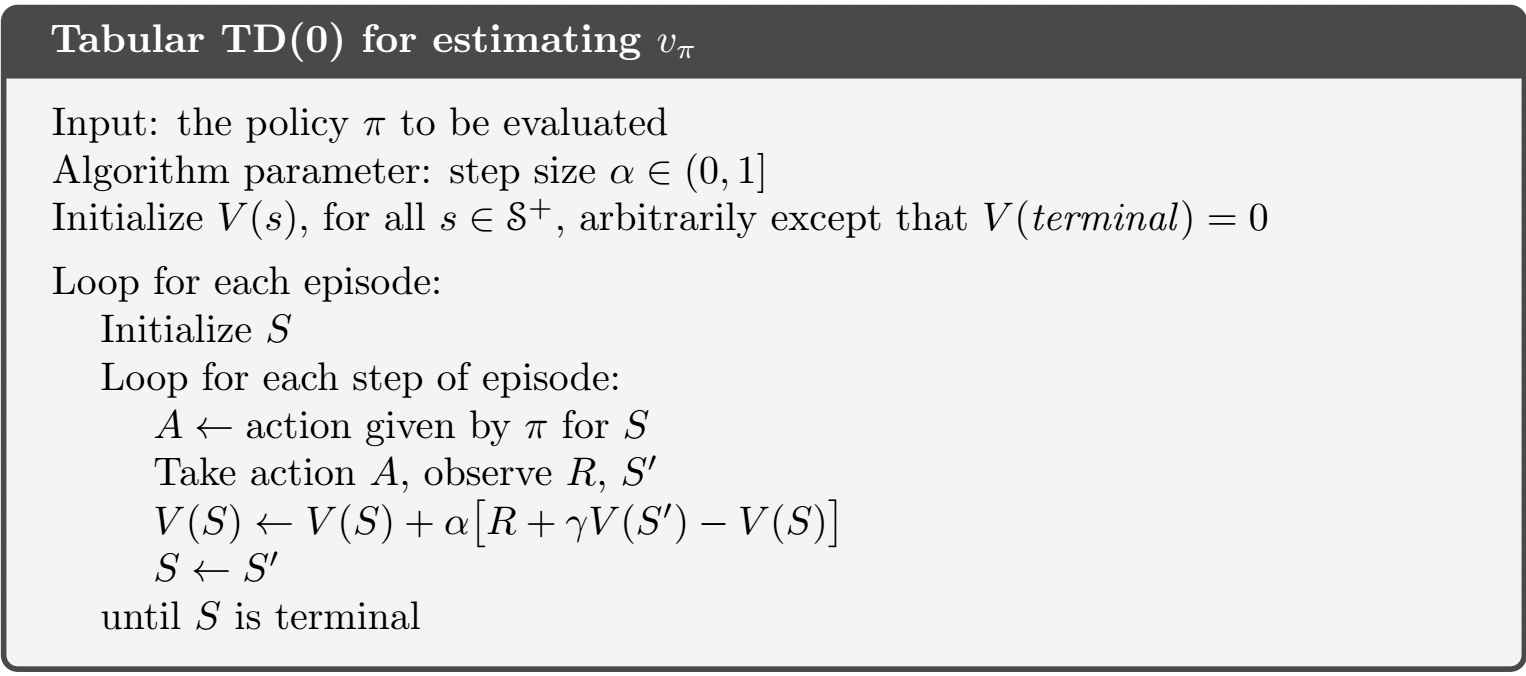
\includegraphics[width=350px,height=200px]{images/tabular_0.png}
        \caption{Tabular TD Sutton Chpt 6}
        \label{fig:my_label}
    \end{figure}
    

The difference here in the bootstrapping mechanism from that of DP is that a single sample of a successor state $V(S^{'})$ is used instead of looking at all possible next states. The quantity in brackets in the TD update is called the TD error and it comes up a lot in reinforcement learning. It is a sort of error because we have a target ($R_{t + 1} + \gamma V(S_{t + 1})$) and we have our estimate $V(S_{t})$. There is an interesting result here that if V(s) is not updated during an episode then we can actually write the Monte carlo error as a sum of TD errors

$G_{t} - V(t) = \sum_{k=t}^{T - 1} \gamma^{k - t}\delta_{k}$

Here $\delta_{k}$ is the TD error. $\delta_{k} = R_{k + 1} + \gamma V(S_{k + 1}) - V(S_{t})$

TD methods have some advantages over MC methods and DP methods. 

* TD > DP because no model of the environment is required. 
* TD > MC methods in that they are naturally implemented in an online, fully incremental fashion. Dont need to wait until the end of an episode. 
* Has similar convergence guarantees as DP and MC. 

Now just like with DP and MC methods we need to go from simply evaluating a policy to having a method for improving a policy. We will use the GPI as before as a framework for achieving this. Just like with MC we focused on estimating $q_{\pi} (s,a)$ which does not force us to have a model of the environment. The TD update can be rewritten in this notation as 

$ Q(S_{t}, A_{t}) \leftarrow Q(S_{t},A_{t}) + \alpha[R_{t + 1} + \gamma Q(S_{t + 1},A_{t + 1}) - Q(S_{t},A_{t})]$

This is an on-policy method since we are using our policy to sample actions $A_{t + 1}$ for our target value. The algorithm below is an example of an algorithm that utilizes this update. We can see that policy evaluation and policy improvement are coupled a bit more tightly than before. We are using the current value estimate Q(s,a) to find a greedy policy that serves as our policy improvement step. Then for policy evaluation we use the update previously described. 

\begin{figure}[H]
        \centering
        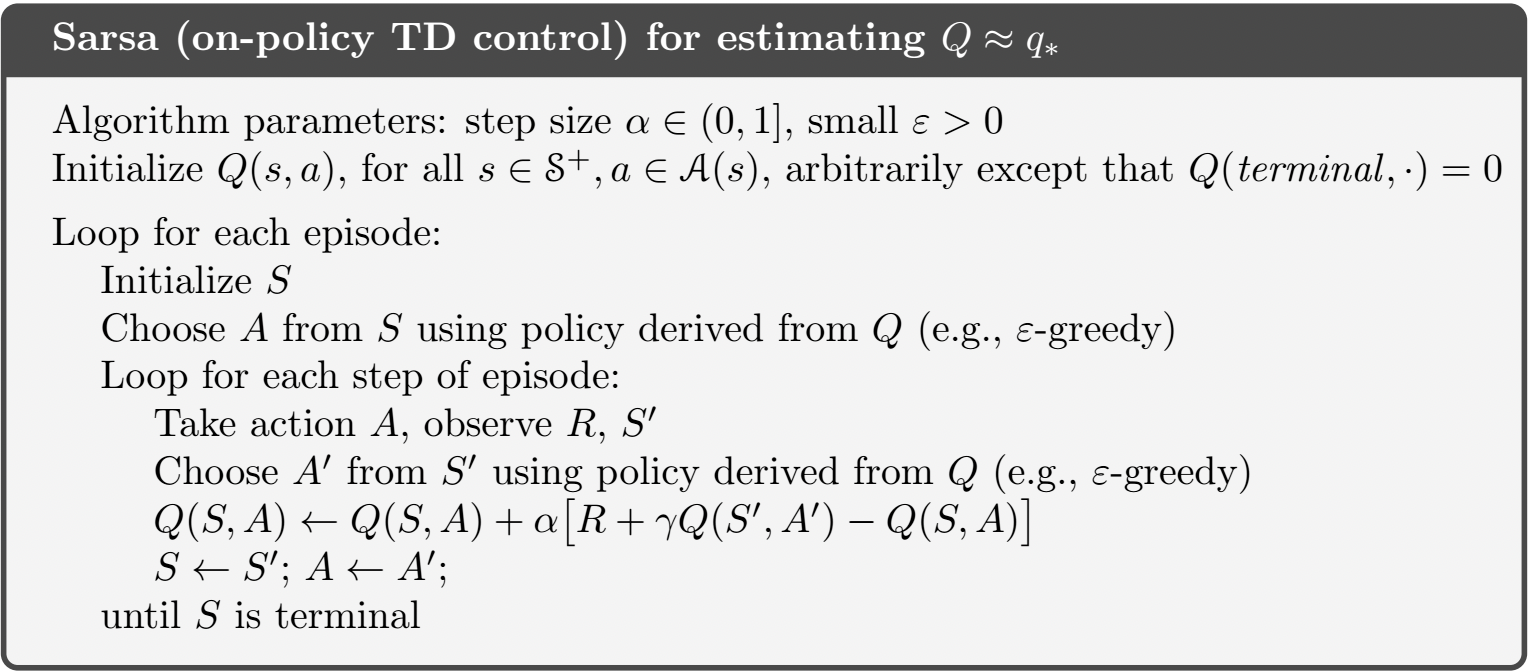
\includegraphics[width=350px,height=150px]{images/sarsa.png}
        \caption{Sarsa: Sutton Chpt 6}
        \label{fig:my_label}
    \end{figure}

A variant of Sarsa is called Q learning and has gained quite a bit of popularity since its recent success with its deep learning variant DQN which we will discuss later. Q learning modifies the TD target by simply taking the max action of the observed next state. So the TD error becomes. 

\begin{equation}
   \delta_{t} = R_{t + 1} + \gamma \: \underset{a}{max}Q(S_{t + 1},A_{t + 1}) - Q(S_{t},A_{s})
\end{equation}

The learned value function in this case directly approximates $q_{*}$. This is because it satisfies the policy improvement theorem by always taking the max action. It also still manages to visit all state action pairs by acting $\epsilon$-greedily from the current state. There have been a lot of nice theoretic work to prove convergence (Watkins,1989). The adjusted algorithm is presented in full below. The change to using the max action in place of an action selected from the policy means that we form a target that does not depend on the policy being used and therefore makes the algorithm an off-policy algorithm. So this off-policy distinction simply means that with off-policy we learn using a different policy than the one we used to take actions with. Q learning has had a lot of success when combine with deep learning which we will look at next. 

\begin{figure}[H]
        \centering
        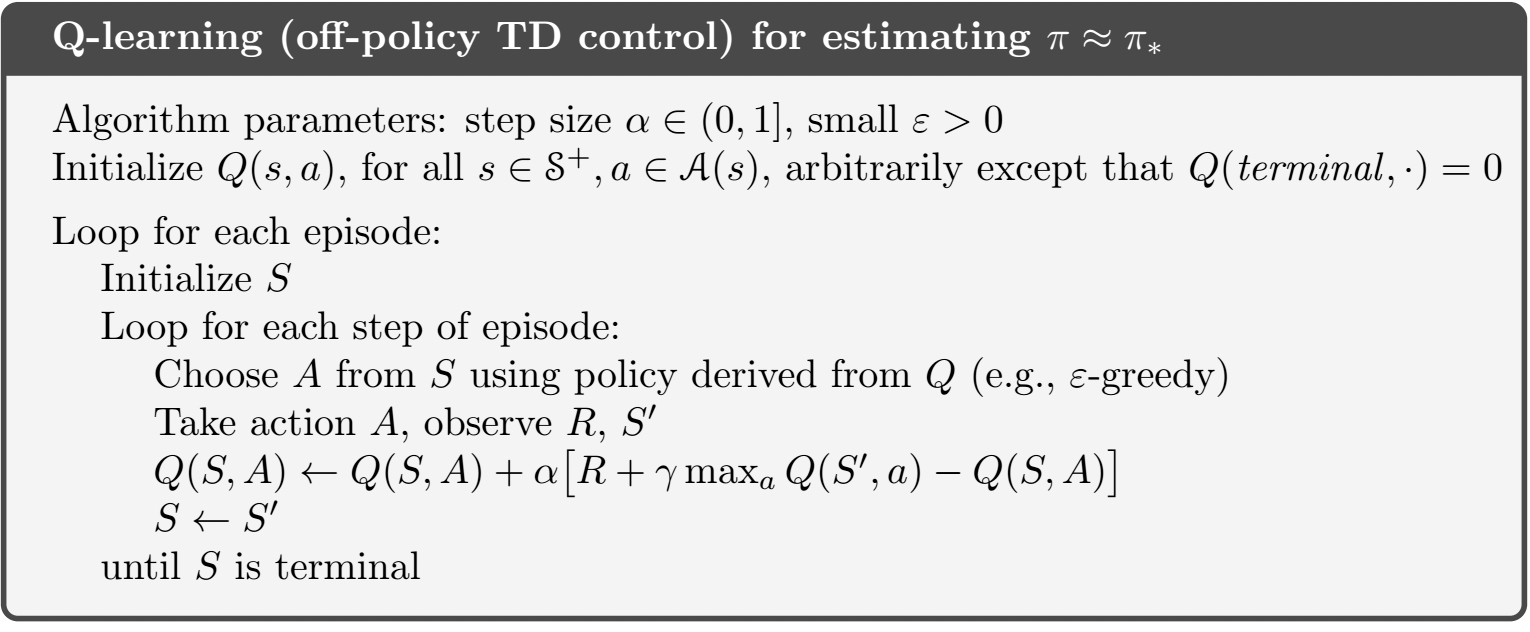
\includegraphics[width=350px,height=150px]{images/q_learning.png}
        \caption{Q learning: Sutton Chpt 6}
        \label{fig:my_label}
    \end{figure}
    
    
\section{Function approximation and Deep RL}

We have seen so far that no matter what the approach to RL is you need someway to evaluate a policy and you need a way to improve a policy. We also identified some of the bottlenecks of various approaches. DP for instance suffers from the "curse of dimensionality" in that as the size of the state space increases the computational requirement grows exponentially. Monte carlo methods and TD learning helped us to get around this by being able to effectively sample and learn from experience. We looked at tabular methods that essentially maintained a lookup table for each state action pair like in Q learning. This has its limits as the state and action space grows. It will become unfeasible to require approximating the value of Q(s,a) for every state and action pair. It requires too much computation to adequately approximate the true $q_{\pi}$ for a given policy. If the state space is large it is reasonable to think that an agent will often encounter states that it has never seen before even after a lot of exploration. What if we were able to generalize the information learned from one state to other similar states? This would allow us to more effectively make use of experience. This task of generalizing from a given set of data to unseen data has been studied quite a bit. Function approximation is the typical approach that helps us to learn from examples. 

Function approximation usually means that we attempt to parameterize a function with a set of learned weights. Parameterizing a function would mean that we take a set of weights $\mathbf{w} \in \mathbb{R}^{d} $ and use them to approximate the true value function $\mathbf{v}_{\pi}$ for a given policy $\pi$. This can be represented as $\hat{\mathbf{v}}(s,\mathbf{w}) \approx \mathbf{v_{\pi}}$. The function $\hat{\mathbf{v}}$ can be something complex like a neural network or something more simple like a linear function. Function approximation helps with generalization in that we now have a set of weights that "represent" the states. Instead of having a separate representation for each state we can represent many states with a lower dimensional representation since typically $d << |S|$. Two states that are similar by some metric will have a similar representation in this new weight space. That means that it should have a similar output as well. So if we have some similarity metric $d$ then if for two states $s_{1}$ and $s_{2}$ we have that $d(s_{1},s_{2}; \mathbf{w}) \approx 0$ then we also should have that $ | \hat{\mathbf{v}}(s_{1},\mathbf{w}) - \hat{\mathbf{v}}(s_{2},\mathbf{w}) | \approx 0$. Thinking to a tictactoe example you would want two board positions that are similar to have similar values. Such as the following two boards. 

\begin{figure}[H]
    \centering
    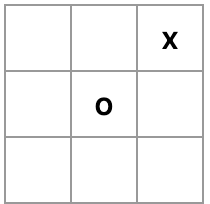
\includegraphics[width=100px,height=100px]{images/t_board_0.png}
    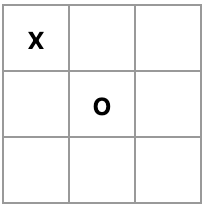
\includegraphics[width=100px,height=100px]{images/t_board_1.png}
    \caption{TicTacToe Board}
    \label{fig:my_label}
\end{figure}
    
Supervised learning is a common function approximation technique used in machine learning in which an algorithm is given a set of data $X$ and some labels $Y$ that are the thing the algorithm is attempting to learn. The goal is to find patterns in $X$ that allow one to be able to minimize some loss function $L(f(X^{'}),Y^{'})$ where the algorithm is represented by the function $f$ and $X^{'},Y^{'}$ is some unseen data but that come from the same distribution as the observed data $X$. Some of the difficulty in applying supervised learning techniques to reinforcement learning is that we actually are not looking at a stationary distribution. The parameters that describe the underlying distribution are capable of changing over time and as the agent interacts with the environment. To further highlight difficulties with using this approach in RL we are generally trying to do policy evaluation  using the current policy $\pi$. This however will be changing as we run policy improvement. So we must use methods that are able to handle the nonstationarity of the problem. 

Nevertheless we can start by phrasing our RL problem as a SL problem. First we need to actually specity our loss function for RL as well. We know that we want to minimize some distance between what our parameterized prediction says and what our target says. We want to specify $L (\mathbf{v}_{\pi},\hat{v}(s,\mathbf{w}))$. A common function for $L$ is the MSE. We can write this as $\mathbf{MSE} = \sum_{s \in S} [\mathbf{v}_{\pi}(s) - \hat{v}(s,\mathbf{w})]^{2}$. We dont have access to the underlying function $\mathbf{v_{\pi}}$ but we can use our target that we have specified in previous examples. In supervised learning terminology we have a target like $G_{t}$ (MC target) or $ R_{t + 1} + \gamma \hat{\mathbf{v}}(s,\mathbf{w})$ the TD target which is like our labels $Y$ and we have the current state $S_{t}$ which is like an observation of $X$

\section{DQN}

We have discussed briefly the idea of applying function approximation to RL. The task is non trivial and we have noted a couple of the dangers involved. I will now use a popular paper to further the discussion of the use of function approximation to enhance the ability of a RL algorithm to better generalize. A nature paper from 2015 entitled "Human-level control through deep reinforcement learning" \cite{dqn} showed how you could take a "simple" algorithm like Q learning and scale it to be a state of the art. Previous work on applying Neural networks to Q learning showed that this approach was unstable \cite{nfq}. The instability comes from several sources. 

\begin{itemize}
    \item Correlations present in the sequence of observations
    \item Small updated to Q may significantly change the policy and therefore the data distribution
    \item Correlations between action-values (Q) and the target values r + $\gamma Q(s^{'},a^{'})$
\end{itemize}

We have already mentioned the second issue which refers to the nonstationarity of the data. The other two refer to a common problem that most supervised learning (SL) problems are forced to address. That is correlation among samples. There is a common assumption made in most SL tasks that the observed samples are IID (Independentally and Identically distributed). A lot of care has to be taken to help at least approximate this assumption.  In the case of Q learning the sequences are highly correlated but so are the labels. The DQN paper addressed these issues in two ways. 

\begin{itemize}
    \item Using an experience replay buffer that randomizes the data
    \item Only periodically update Q and maintain a target network. 
\end{itemize}

The first helps to solve the first two problems. It helps remove correlation in the observations through random sampling of a replay buffer. We will discuss the details of the replay buffer shortly. The randomization also helps to solve the nonstationarity problem as it smooths out the data distribution. DQN only periodically updates the Q function which helps to remove correlation with the target values. Since a separate network is maintained for making target predictions this means that the target values remain much more stable. 

DQN uses a neural network to parameterize the state-action function $Q(s,a) \rightarrow Q(s,a,\theta_{i})$. Here $\theta_{i}$ signifies the parameters of the network at iteration $i$. Recall from our discussion of Q learning that the TD error had the form $\delta_{t} = R_{t + 1} + \gamma \: \underset{a}{max} Q(S_{t + 1},A_{t + 1}) - Q(S_{t},A_{t})$. In the DQN paper they translate this to a differentiable loss function as follows. 

$ \mathbf{L_{i}}(\theta_{i}) = \mathbb{E}_{s,a,r,s^{'} \sim \: U(D)} [(r + \gamma \: \underset{a}{max} Q(s^{'},a^{'};\theta_{i}^{-}) - Q(s,a;\theta_{i}))^{2}]$

The $\theta^{-}$ weights are the weights for the target network. This is simply the mean squared error of the target and predicted values using the parameterized version of the Q function. Note how the target value depends on the prediction of the target network. This is really a large distinction between reinforcement learning and supervised learning. A picture of their network used is given below. They evaluated their agent on Atari games and used a convolutional neural network for the parameterized Q function. The output of the network that you see on the far right is the set of possible actions with each of the corresponding values. 

\begin{figure}[H]
    \centering
    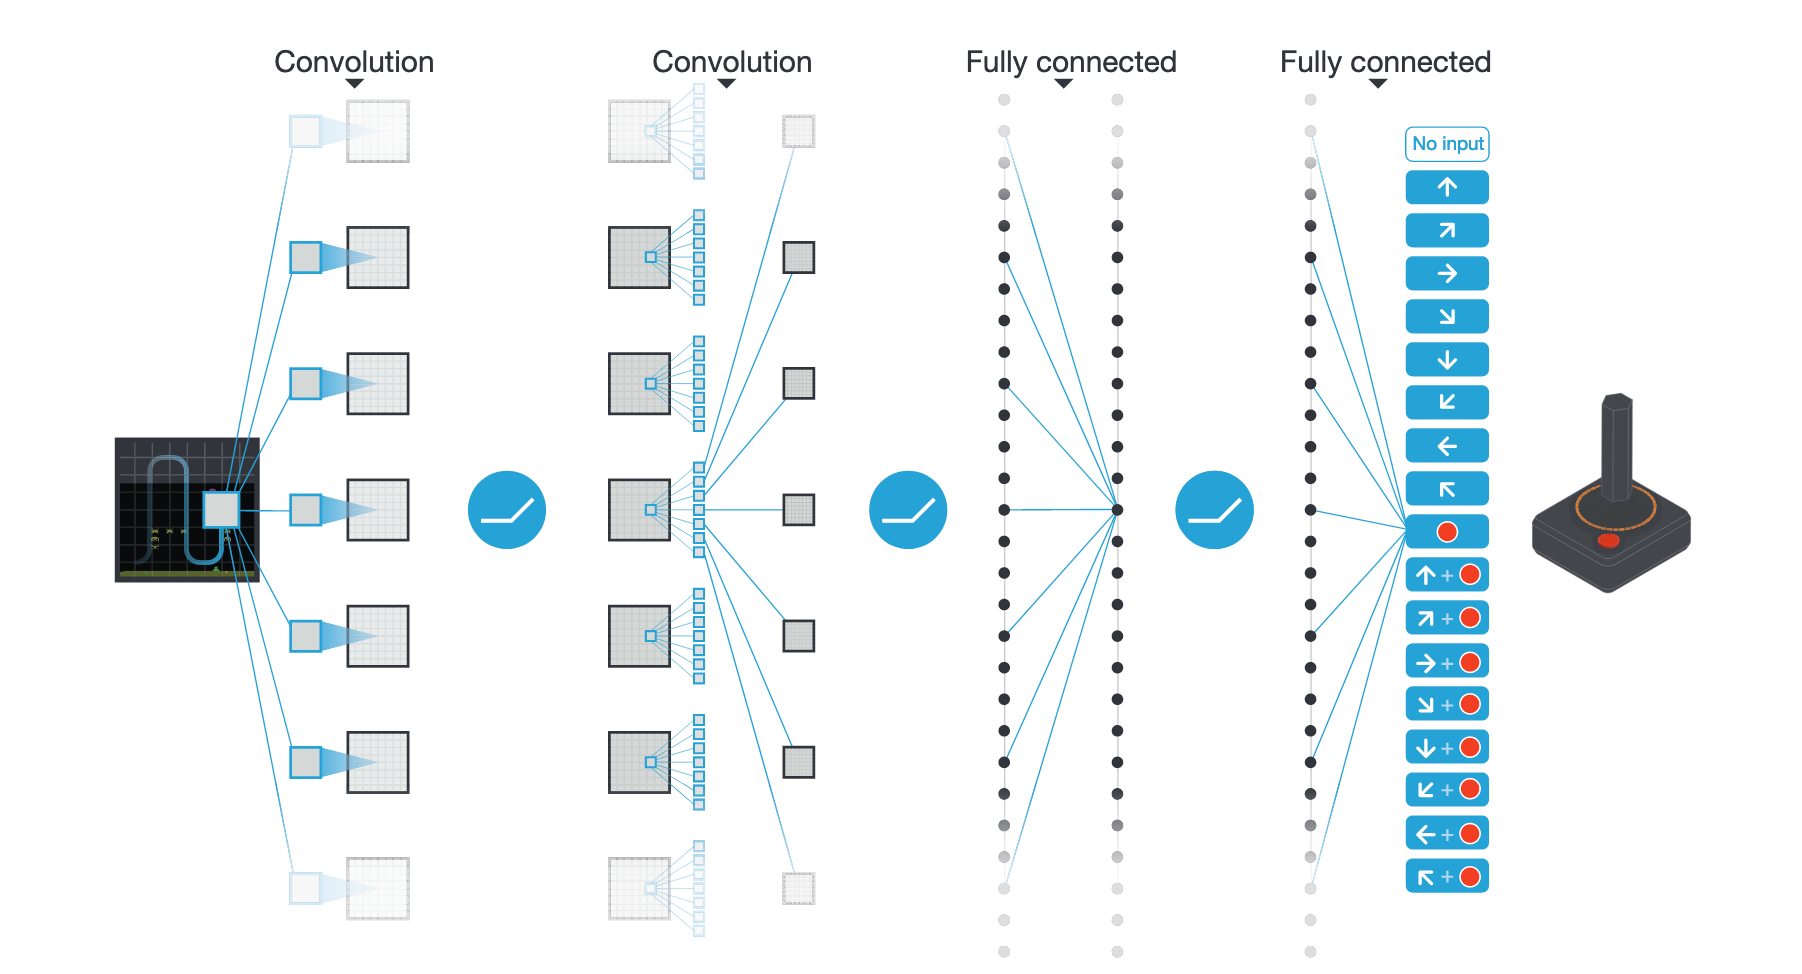
\includegraphics[width=350px,height=200px]{images/DQN_architecture.png}
    \caption{DQN architecture}
    \label{fig:my_label}
\end{figure}

Prior to looking at the algorithm in full lets look at two of the more important components that made DQN successful. First the target network being used requires a bit more explanation. To be clear its not actually a separate network. It is simply weights of the Q network at prior iterations. So it is basically "old" weights. We specify the number of iterations that we wait to update the target network up front as a hyper parameter. When we do finally update the target network we simply copy the current network weights and use them as our new target. This does not completely fix the nonstationary problem since in all RL algorithms that bootstrap we will always have some amount of variability in the target distribution. 

We also need to look at a what an experience replay buffer is. The experience replay buffer is essentially a database of experience. While the agent interacts with the environment data that is generated from that interaction is stored away. Then to update the network batches of experience are randomly sampled from the buffer. The fact that the experience is sampled randomly is significant in that it helps to decorrelate the data and stabilize training. Experience is typically stored in the form ($s_{t},a_{t},r_{t},s_{t + 1}$). The current state, action, reward and the next state that the agent transitions to after taking action $a_{t}$. A replay buffer will be used in the AlphaZero algorithm so keep it in mind going forward. 

The algorithm from the paper is in the figure below. Lets go through each one of the steps. It might look complicated but it is really quite similar to Q learning that we have seen plus some deep learning magic. 

\begin{figure}[H]
    \centering
    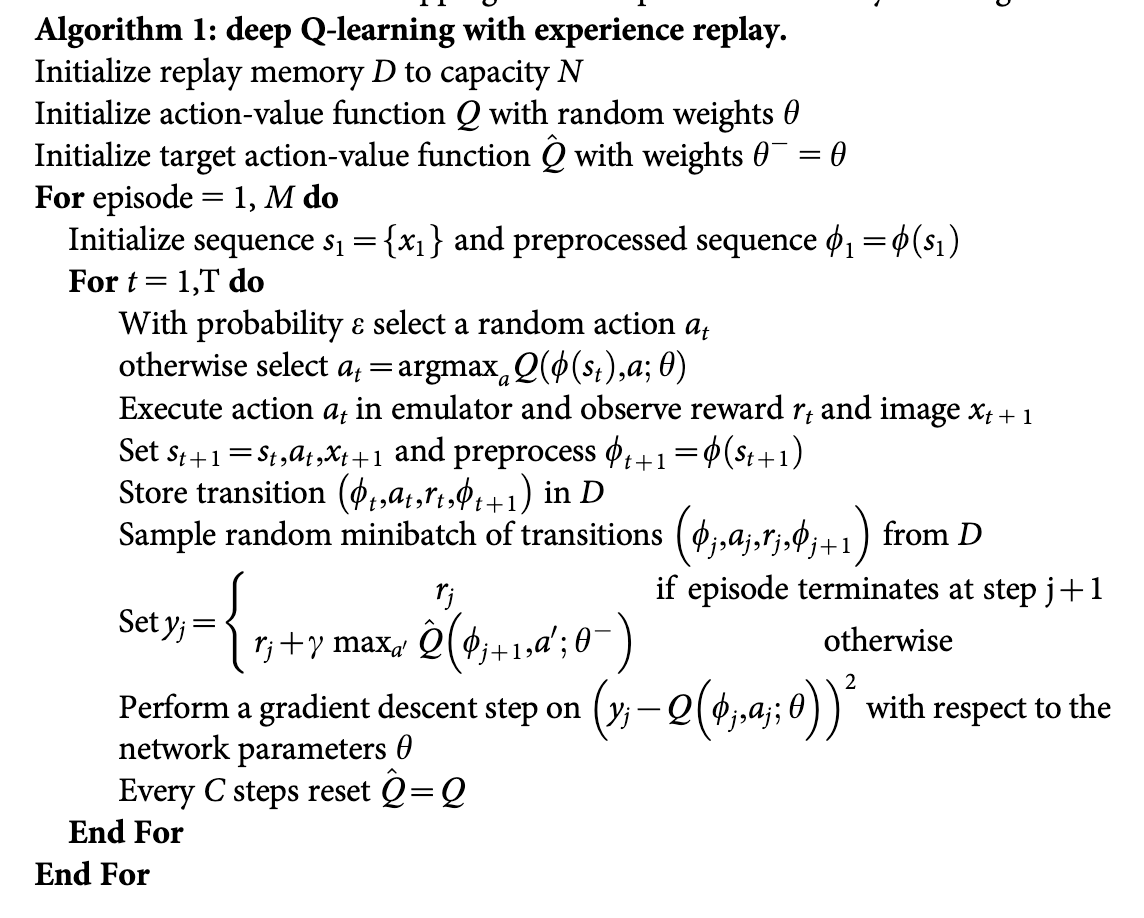
\includegraphics[width=350px,height=200px]{images/DQN_algo.png}
    \caption{The DQN algorithm}
    \label{fig:my_label}
\end{figure}

\begin{enumerate}
    \item Initialization - We simply initialize the weights of the network randomly and then set the target weights to a copy of those weights. We also initialize the replace buffer which simply means instantiating whatever data structure your using to hold the data such as an array.  
    \item Inside the main for loop we get the initial sequence. A sequence here is a stack of the 4 most recent frames. Then the function $\phi(s_{t})$ scales those frames to be of size 84 x 84. 
    \item The second for loop takes us through each step of the episode. We use an $\epsilon$-greedy strategy to select an action. The action is executed against the environment and the reward and next state are observed and processed. 
    \item We store the current data into the replay buffer. 
    \item We train our network on a random sample of transitions from our replay buffer using gradient decent and the previously discussed loss function. 
\end{enumerate}

Thats really it. This is something that you can code up in less than 150 lines of python code using a modern machine learning framework like pytorch or tensorflow. This seemed like a nice elegant algorithm that utilized deep learning to reach state of the art performance on difficult tasks like the Atari games. So why not use this same approach to solve something like Go? There is something that this approach still suffers from. It has difficulty with the credit assignment problem and stability in sparse reward regimes. The credit assignment problem in RL is the problem of knowing whcih action in which state was responsible for a particular outcome. In a game like Go you will generally take many many actions prior to the end of the game and wont receive any feedback until the game is complete. This is what is meant by sparse rewards. The lack of informative feedback from the environment. Once the game is complete you will know wheter you won or lost (+1,-1). Then how do you inform the network which states and actions were responsible for the outcome? In theory its not totally obvious why the Deep Q learning algorithm should not be able to overcome these issues. In absence of better theory however we must be content with the empirical evidence that points to DQN's instability in these regimes. We now will discuss the idea of planning and how that helps to overcome this problem. AlphaZero is a complex planning algorithm so we will start with something a bit more simple. 

\chapter{Search}

    \section{Adversarial Search}

The idea of adversarial search is when you have two or more agents with conflicting goals acting in the same environment. Games provide a nice test-bed for these types of algorithms. The hope is that we can learn concepts that will transfer to more complex environments or at least point us in the right direction. In this paper we will just be interested in discussing two player perfect information zero sum games. The ``zero sum" refers to the fact that any loss or gain of one player will directly come at the gain or loss of the other player. Perfect information refers to the notion that ``each player, when making any decision, is perfectly informed of all the events that have previously occurred, including the initialization event of the game. As in chess the board is observable to both players and so there is no hidden information. This is using the language of game theory. Game theory can approach multi agent environments from a number of angles but the most popular and effective one is to explicitly model the adversarial agents. The other option would be to include the agents as part of the environment and then attempt to model the environment. The first option mentioned works well in the two person zero sum setting and that is the one we will focus on in this paper. 

\section{Self-Play}

Self-play is a concept that has been around in AI for a long time depending on how liberal your willing to be with the term AI. In 1951 Brown came out with a paper describing fictitious play a self-play algorithm In 1959 Checkers was solved using self-play with expert knowledge. There have been many other successes including AlphaZero. Self-play in short is any algorithm for which there are 2 or more players and the agent makes actions for every player. So the agent just plays against itself and improves play based off of what it observes during this self-play. This is easiest to see in zero sum two player games since they are symmetric. In this setting a self-play algorithm will play as both player 1 and player 2.The agent will play against itself switching perspectives between player 1 and player 2. AlphaZero does just this. We do this as humans occasionally when playing a game or perhpas other activities. For instance when thinking about how to develop better chess strategies you might see how well a strategy does by attempting to play against that strategy yourself and observing the outcome. 

\section{MiniMax and Alpha Beta Pruning}

The MiniMax algorithm is a classic game tree search algorithm. It can be used to arrive at guaranteed optimal solutions in two player zero sum games. 

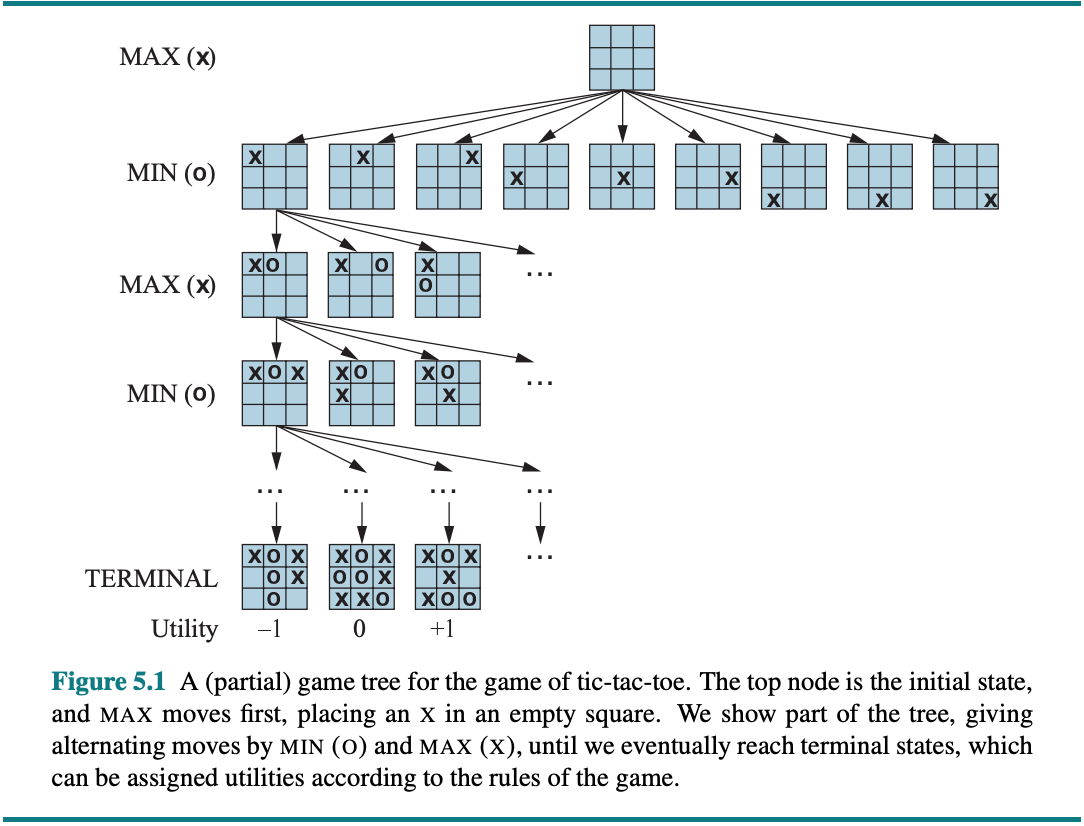
\includegraphics[width=350px,height=200px]{images/aim_figure_5_1.png}

Looking at figure 5.1 above taken from the classic text ``Artificial intelligence a modern approach" [2] we can view the game tree of a two player game as a game between a player MAX and a player MIN. It is player MAX's turn and he wants to maximize his utility. MIN knows that MAX is a greedy human and will be taking actions to maximize his own reward. What should MIN do? MIN will then take actions that will minimize the utility of MAX. MAX in turn knows about the devious plans of MIN and will take actions in accordance with this knowledge. That is to say that each player will act assuming that the other acts optimally. This setup gives rise to our first game-tree algorithm  
The optimal strategy of a given game tree can be determined by working out the minimax value of each state in the tree. The minimax value is the utility for the 
The MiniMax algorithm is the first game tree algorithm that we are going to look at. It is relevant for pedagogical purposes but we will also later use MiniMax as a baseline for comparison vs our more complex agents such as MCTS and AlphaGoZero. 

MiniMax Search Example: The example below demonstrates the algorithm with an oversimplified example. Moving left to right sarting with the max player. The leaf node values are already known. 

\begin{enumerate}
    \item Max player looks for max action over children nodes.  
    \item No value exists on the children nodes so MIN player finds the min action of the terminal states. First for the left node. Than the right. 
    \item MAX can now calculate the max of MIN's nodes. So in this toy example it is concluded that MAX should take the right action. 
\end{enumerate}

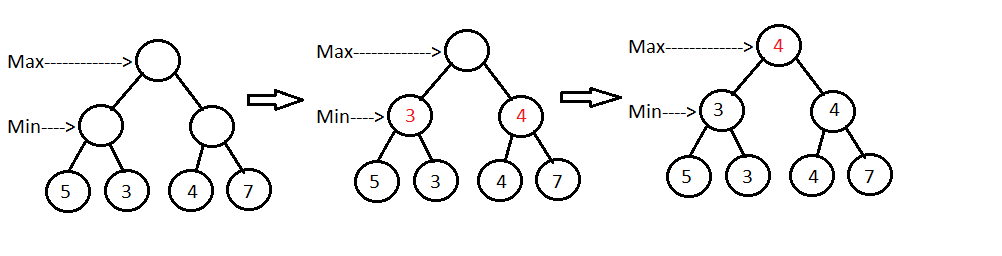
\includegraphics[width=300px,height=100px]{images/minimax_example.png}

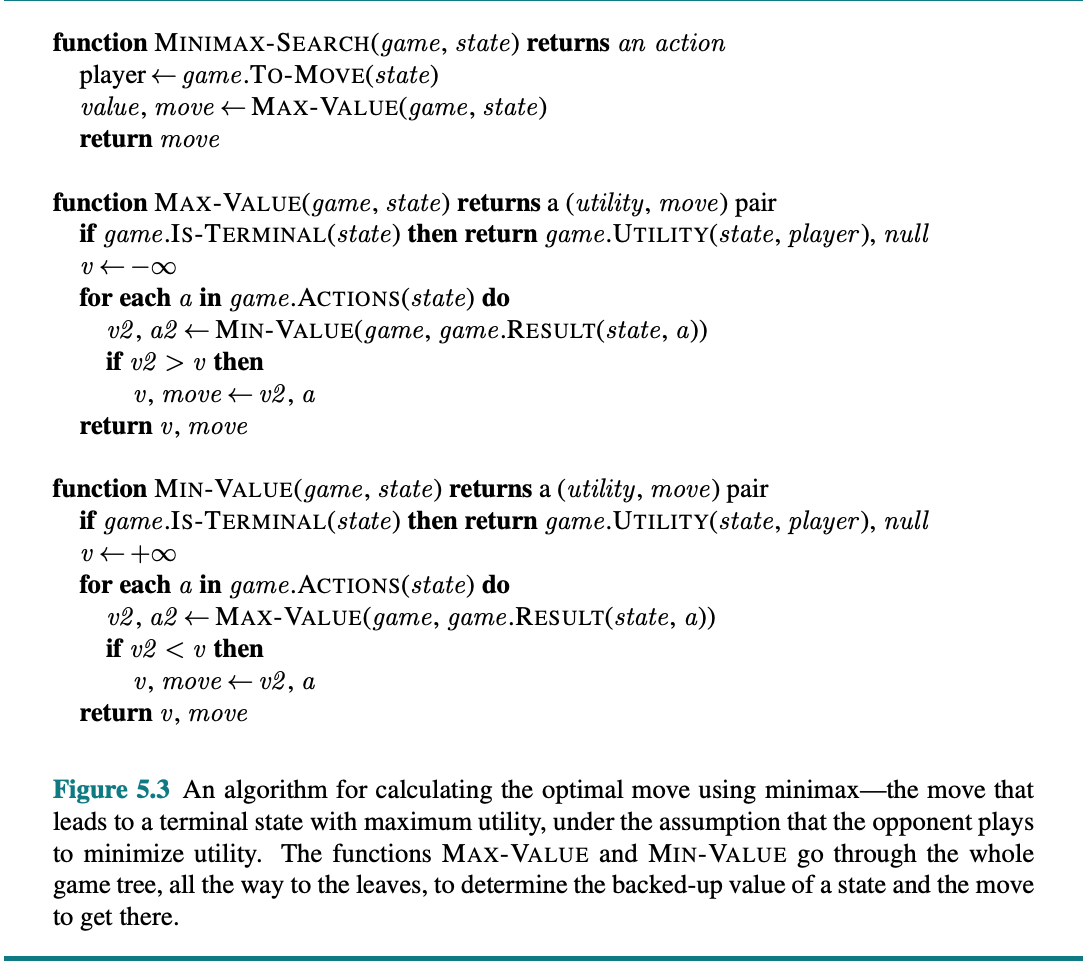
\includegraphics[width=300px,height=200px]{images/minimax_algo.png}

The pseudocode for the algorithm above can be implemented almost completely with three functions and a tree representation of whatever space your interested in. This algorithm is guaranteed to give you the optimal solution but is quite computationally expensive as every node needs to be visited at least once. One way to help reduce the search space is with alpha-beta pruning. The basic Idea of the algorithm is that there are points during the minimax search that searching further down a particular path is unnecessary to reach the optimal minimax decision. 

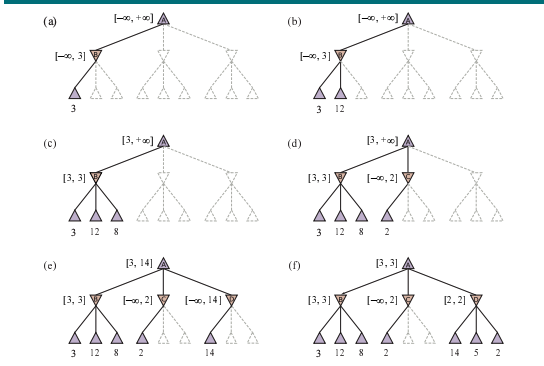
\includegraphics[width=300px,height=200px]{images/alpha_beta_figure.png}

The above figure [2] (fig 5.5) gives a nice example of why you dont need to search the entire tree. Let the two unsearched children nodes of node C be x and y respectively. Then the Minimax evaluation of the root node of the tree following the steps we just learning is evaluated like the following 

$ MINIMAX(s_{0}) = max(min(3,12,8), min(2,x,y), min(14,5,2)) $

$ = max(3,min(2,x,y),2) = 3 $ since $ min(2,x,y)$ will never evaluate to anything larger than 2 and 2 is less than 3 then the max player will never select node C and it is unecessary to know what x and y actually evaluate to. The figure below demonstrates this idea nicely. Consider the node n, if another node at the same level as n say $ m^{'}$ or another node further up the tree $m$ is better than n than we dont need to continue to explore n further. So as soon as we have enough information about $n$ to make this conclusion we can stop and prune whatever is left of $n$. Alpha-beta search as the name implies uses to values to help us know when pruning can take place.

\textbf{Alpha} - The value of the best choice we have found so far at any choice point along the path for MAX. 

\textbf{Beta} - The value of the best choice we have found so far at any choice point along the path for MIN. 

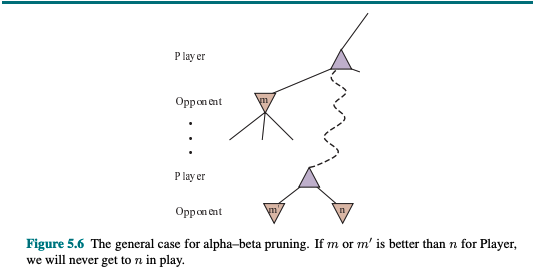
\includegraphics[width=400px,height=200px]{images/AI_figure_5_6.png}

Another nice way to represent this constraint is with the following graphic. Any node we are considering must be able to be between alpha and beta as represented by the number line. $ \alpha \leq N \leq \beta $

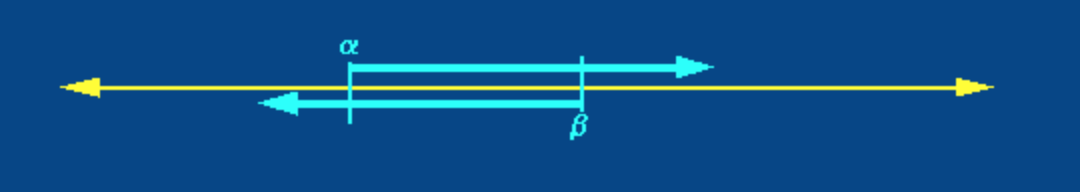
\includegraphics[width=400px,height=100px]{images/alpha_beta_number_line.png}

\section{MCTS}

Here we will describe MCTS in its entirety. It is such an essential part of AlphaZero that it needs to be understood well. We will introduce some new vocabulary in this section as MCTS builds off of previous ideas in RL that are not obvious just from the description of the algorithm. I think it helps to start by seeing the algorithm in its entirety. The algorithm alternates between planning and acting. The planning step consists of a guided search through state space and the acting step consists simply on choosing the best action based on what happened during the planning step. The figure below gives a nice pictorial representation of the four main steps of the planning step. States are represented as white nodes and black circles as possible actions.    

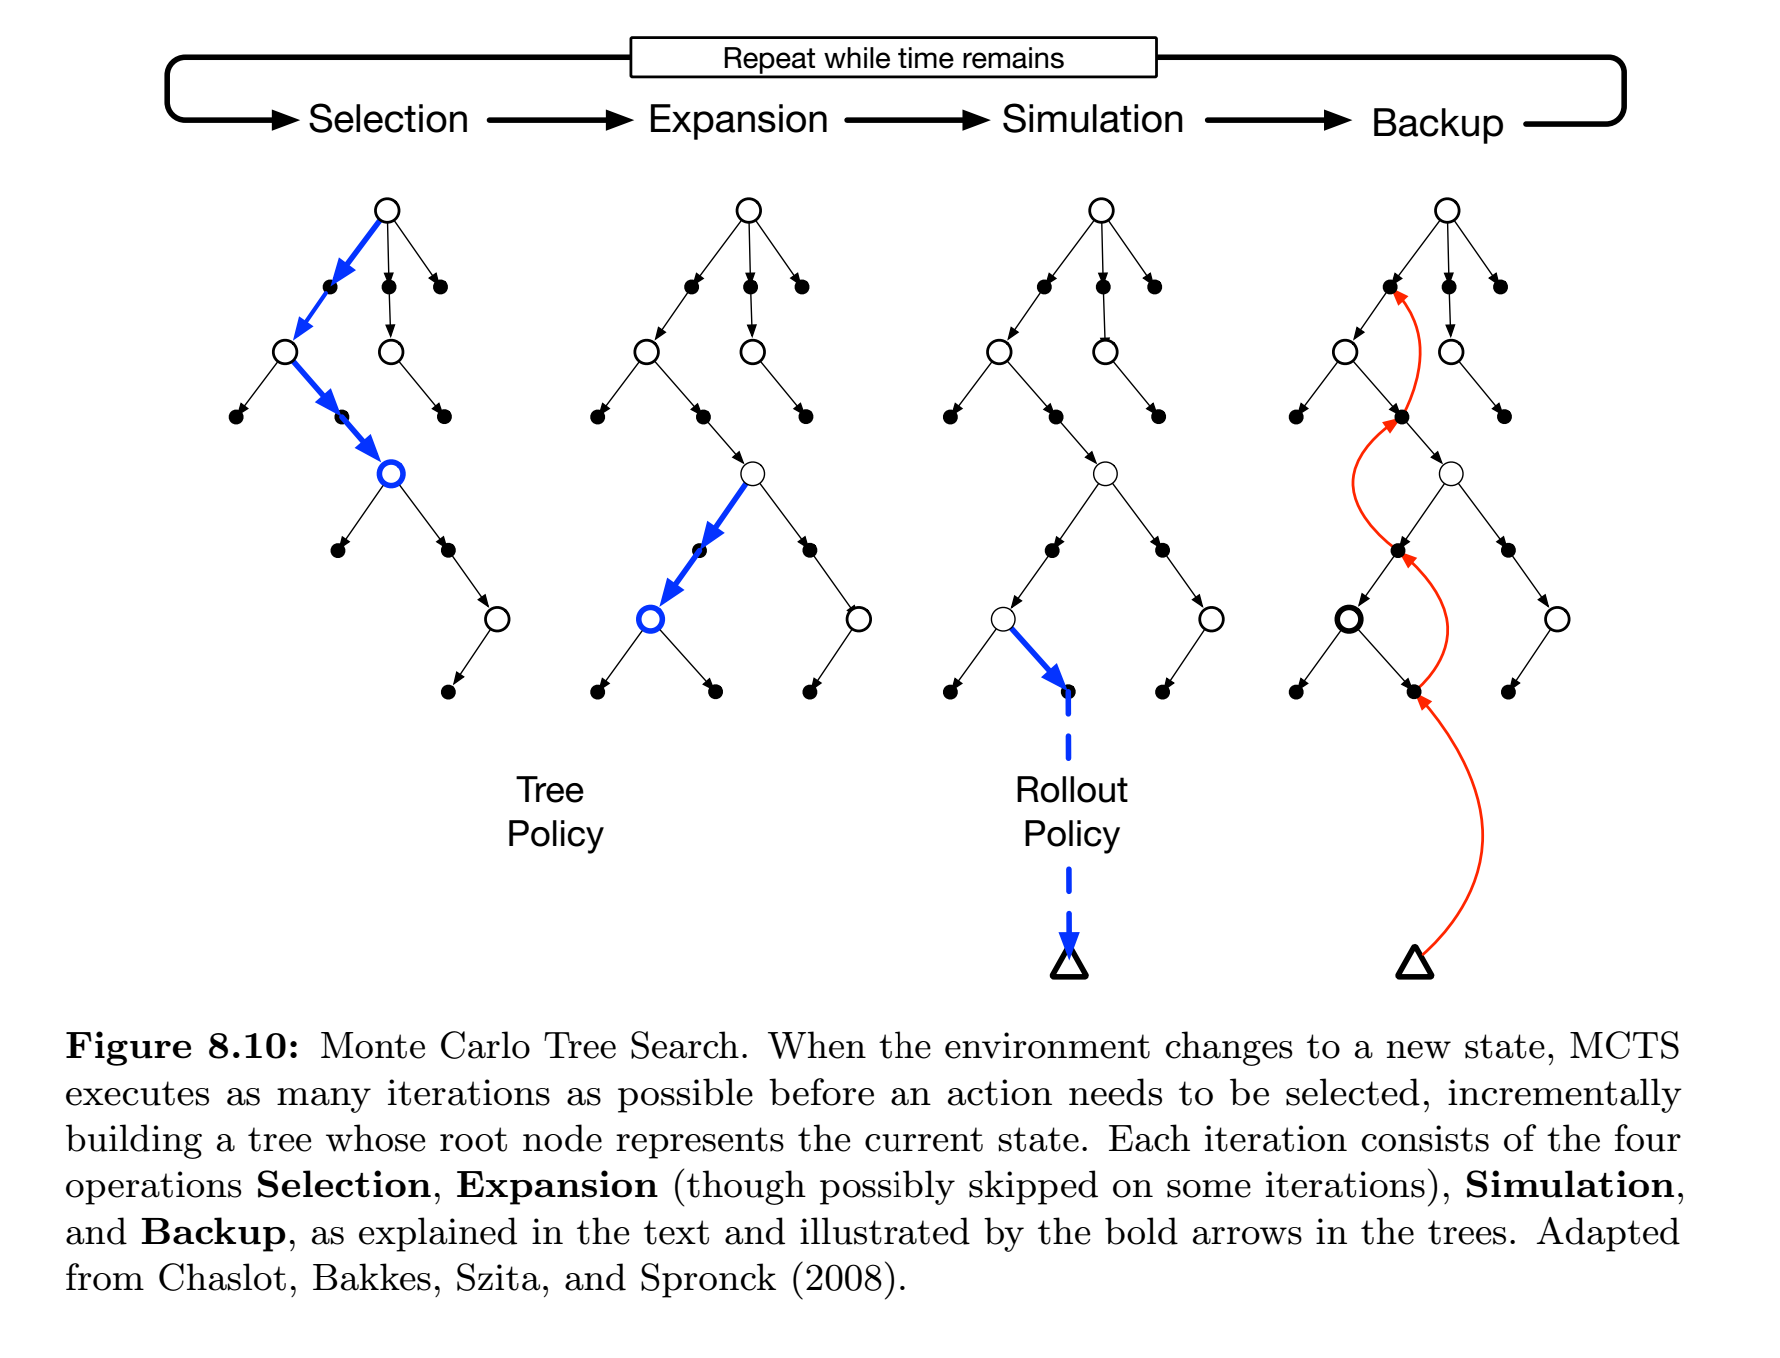
\includegraphics[width=450px,height=300px]{images/mcts}

The goal is to find the path through state space that will yield the highest return on average. You start with a game tree that only contains the root node. In the case of Go this would be the node representing the start of the game. You then proceed and repeat the following 4 steps as are represented in figure-1 for some predefined number of iterations. Once you have completed all iteration you will move on to the action phase in which you use the statistics built up in the tree to select an action in the actual environment. Each node in the tree associate with a unique state from the environment has the following statistics. For each possible action from the current state the state action value is represented by $Q(s,a)$. Visit count values for each state and action is represented by $N(s,a)$.

\begin{enumerate}
    \item \textbf{Selection}
    In this phase of the algorithm child nodes are selected until a leaf node is reached. Leaf node here means either a terminating node (game ending node) or a node that has not been explored yet. The child nodes are selected based on values of the edge connecting parent to child. This value can be assigned in different ways. An example is UCT (Upper confidence bound 1). The way exploration vs exploitation is balanced is using the following formula. 
    
    $ UCT = Q(s,a) + c*\frac{\sqrt{\sum{N(s,b)}}}{N(s,a) + 1} $
    
    includegraphics[width=300px,height=100px]{images/uct.png}
    
    \item Expansion
    
    Once a leaf node has been reached as long as its not a terminating node than add one or more child nodes of that leaf node to the tree. 
    \item Simulation
    
    From the selected child node run a simulation to the end of the episode (game). The simulation decisions use a rollout policy (off policy. Sometime uniform random) to select actions. This is usually done multiple times. So from the current selected node you would just select random actions until the game ends and save the result. You would repeat the process some number of times and then the average of those rollouts would be used as the estimate for the new node. 
    
    \item Backup
    
    The reward returned from the simulation is backed up through the edges of the tree that were used during the current episode. The reward is not saved to states that exist beyond the current tree. If the simulation step is run more than once then the average from the simulation step is backed up through the tree. If you are running MCTS for a two player game than you would flip the value of the return for the opponent node. If the node is a player one node for instance than all  player 2 nodes would get the negative of whatever player 1 received from the simulation outcome. If that was confusing we will see some examples that will help clarify. 
    
\end{enumerate}

As stated before these 4 steps would continue for a predefined number of iterations and then the acting step would commence. Remember those for steps were a \say{thinking} phase where from the current state the algorithm is thinking about what to do. Once the thinking phase is over the agent acts by selecting an action based off statistic in the tree. One common one is to select the action with the most visit counts or the action with highest value. 

Monte Carlo tree search is a decision time planning algorithm. A decision time planning algorithm is one in which a full simulation of planning is run on every state to produce each action. This is in contrast to \textit{background planning}. In background planning a policy or value function is gradually learned by simulated experience. The learning might happen at different time intervals. In short the two differences are this, decision time planning uses simulated experience to select an action in the current state whereas background planning uses simulated experience to improve a policy or value function and then uses that improved policy or value function to then select an action. 

For me this definition was a bit confusing and I suppose that there is likely some overlap in the two approaches in different algorithms. MCTS is a decision time algorithm because from the current state $S_t$ you might run the above 4 step 1k times or 10k times to accumulate statistics in the tree. Then once those simulations are over you will select an action from $S_t$ using the statistics accumulated in the tree. The mechanism for selection can be different from algorithm to algorithm. You might just select an action by trying to maximize value or you might take into account the number of times an action has been taken from $S_t$ in the past.

MCTS is also considered a rollout algorithm. \say{Rollout algorithms are decision-time planning algorithms based on Monte Carlo control applied to simulated trajectories that all begin at the current environment state. They estimate action values for a given policy by averaging the returns of many simulated trajectories that start with each possible action and then follow the given policy}.
(Sutton Page 152). 

(Leaving this out)
I list a few interesting properties that make MCTS a desirable algorithm.
\begin{enumerate}
    \item Planning time is independent of the size of the state space
    \item Need lots of samples to get a good estimate
    \item Running time is exponential in the horizon size. $O(|A|*n)^{H}$ where $A$ is the actions space. $n$ is the number of samples you want to run per simulation. $H$ is the horizon size
\end{enumerate}

\subsection{Example 1}

We will go through a quick toy example to understand each of the steps in MCTS. 
Below is a tree representing some game between two players blue and red. The current node of interest is the root node with value $ 5 / 10 $ (value / count) . 

We start in the select phase and the node has three actions (children nodes) to choose from. Using the UCT algorithm given above the algorithm would ascribe the following values to each node. Starting from the left most node and working right. Let $ c = 1 $

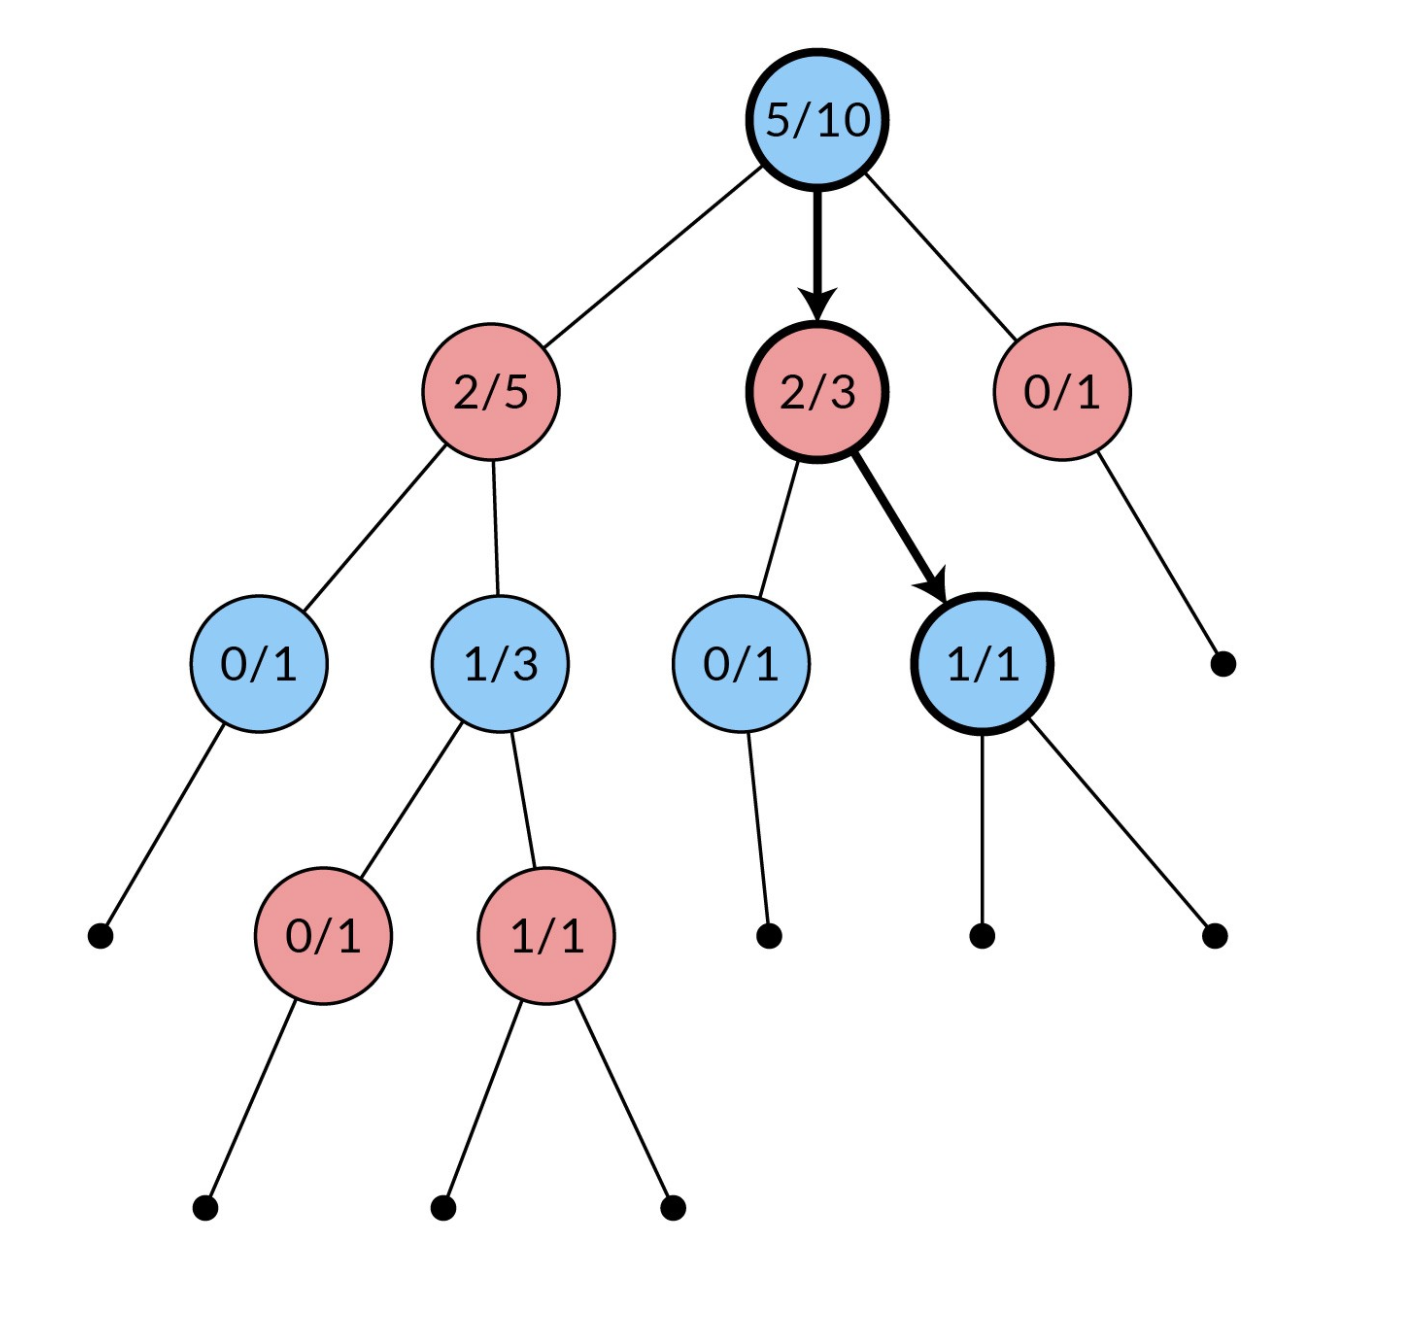
\includegraphics[width=200px,height=200px]{images/mcts_selection.png}

UCT(node1) = $ \frac{2}{5} + c \sqrt{\frac{ln({10})}{2}} = 1.07$

UCT(node2) = $ \frac{2}{3} + c \sqrt{\frac{ln({10})}{3}} = 1.54$

UCT(node3) = $ \frac{0}{1} + c \sqrt{\frac{ln({10})}{1}} = 1.51$

So we select node2 as is indicated with the bold arrow. Now for the children of node2 (node4,node5)

UCT(node4) = $ \frac{0}{1} + c \sqrt{\frac{ln({3})}{1}} = 1.048$

UCT(node5) = $ \frac{1}{1} + c \sqrt{\frac{ln({3})}{1}} = 2.048$

So we select node5 and since node5 is a leaf node we go to our expansion step.

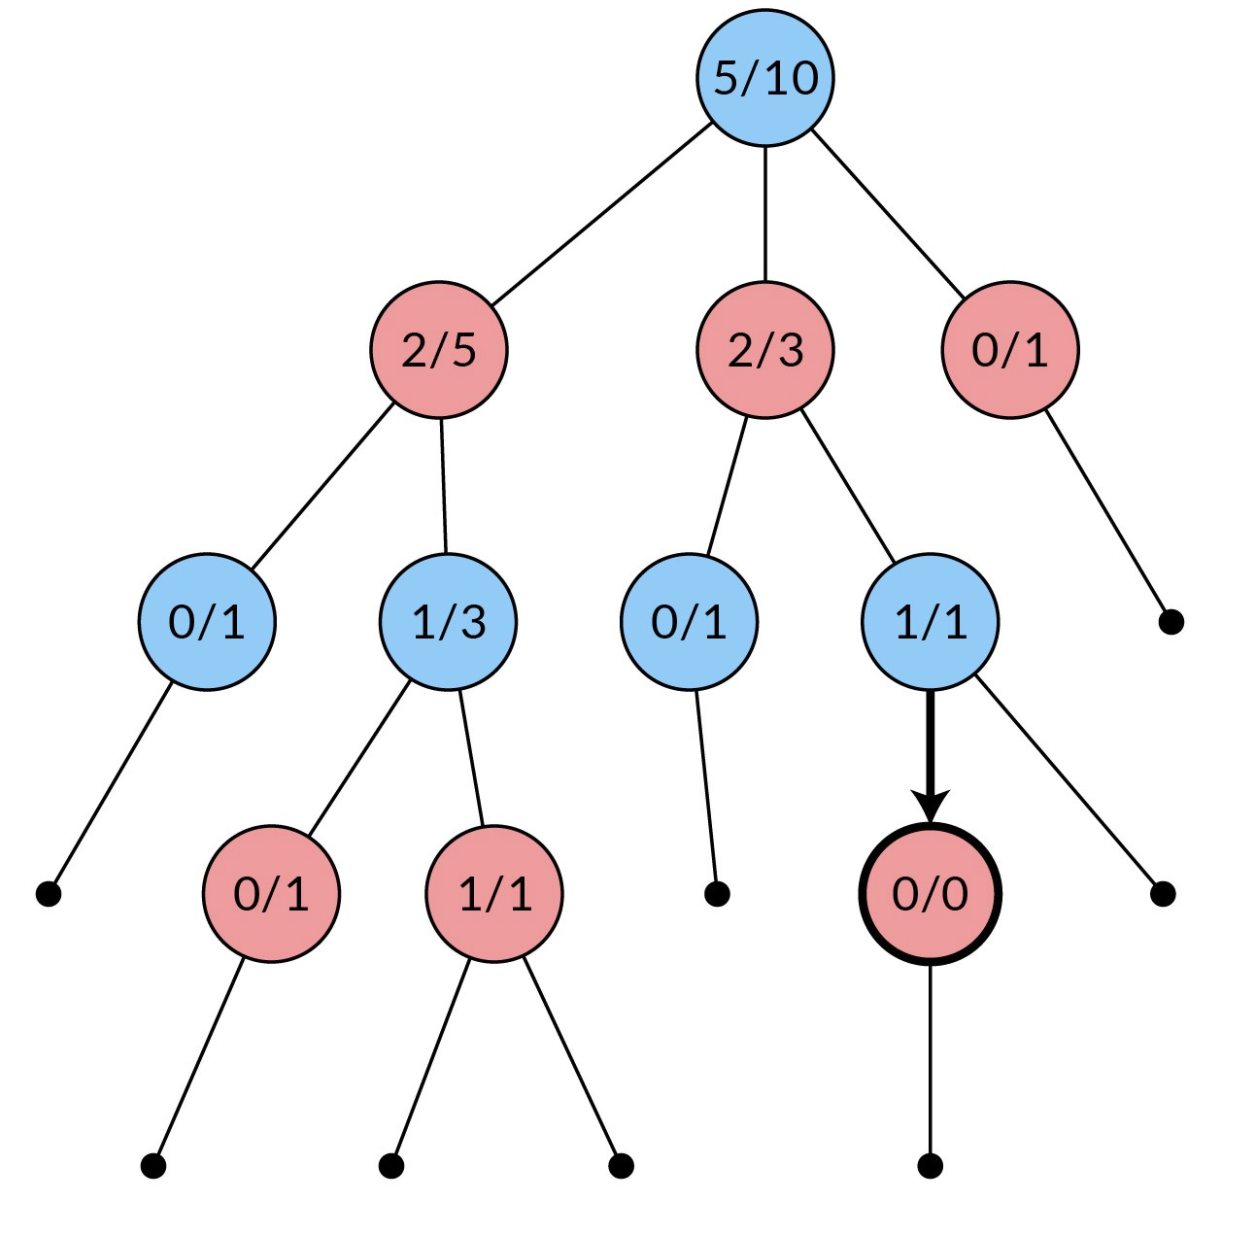
\includegraphics[width=200px,height=200px]{images/mcts_expansion.png}

We randomly select one of the two child nodes and assign the new node values of 0 / 0 (value / count). Now to estimate the value of the new node we run a rollout policy. This is usually random and so the agent will select random actions until a terminal node is reached. 

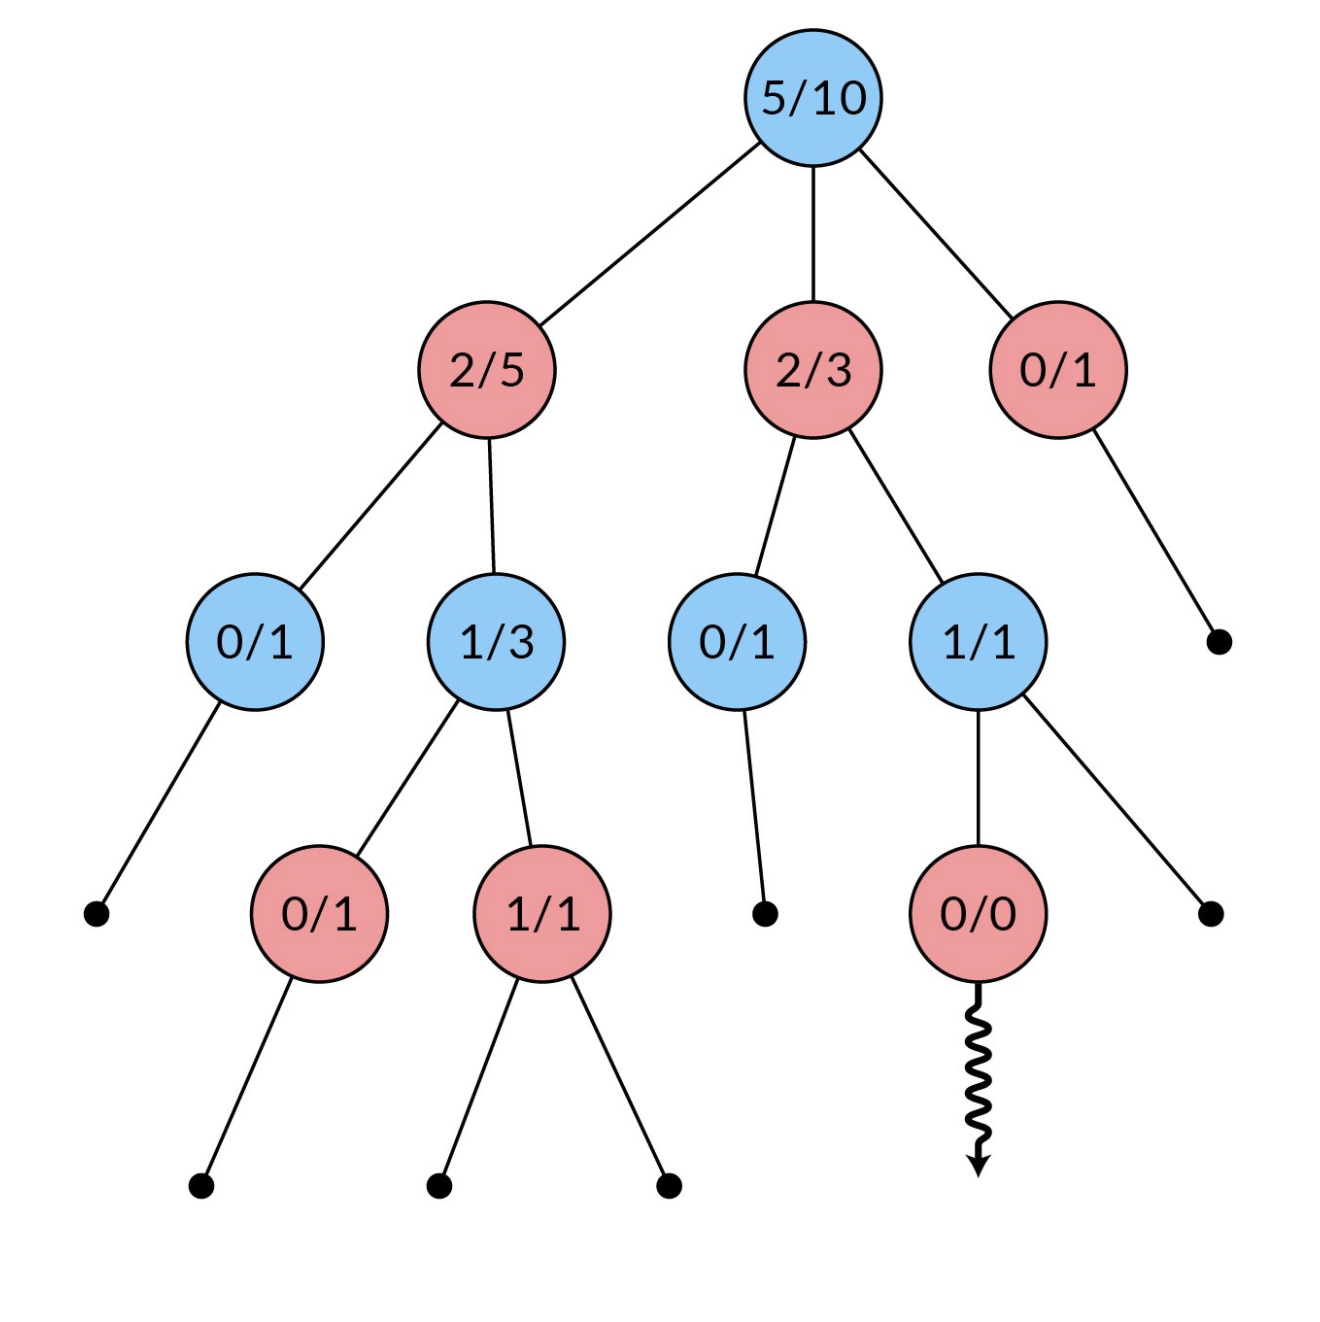
\includegraphics[width=200px,height=200px]{images/mcts_simulation.png}

In this example the terminal node was a win for blue and so now we can back up the values of the tree with this new result. Somewhat counter intuitively since blue wins that means we increase the value of all the red nodes along with their count but only increase the count values of all the blue nodes. This is because the red nodes are actions selected by blue and therefore since blue won that child node is more valuable to blue in the future. This is unique to multi player MCTS and you would not have to worry about this in a non-adversarial or cooperative setting. 

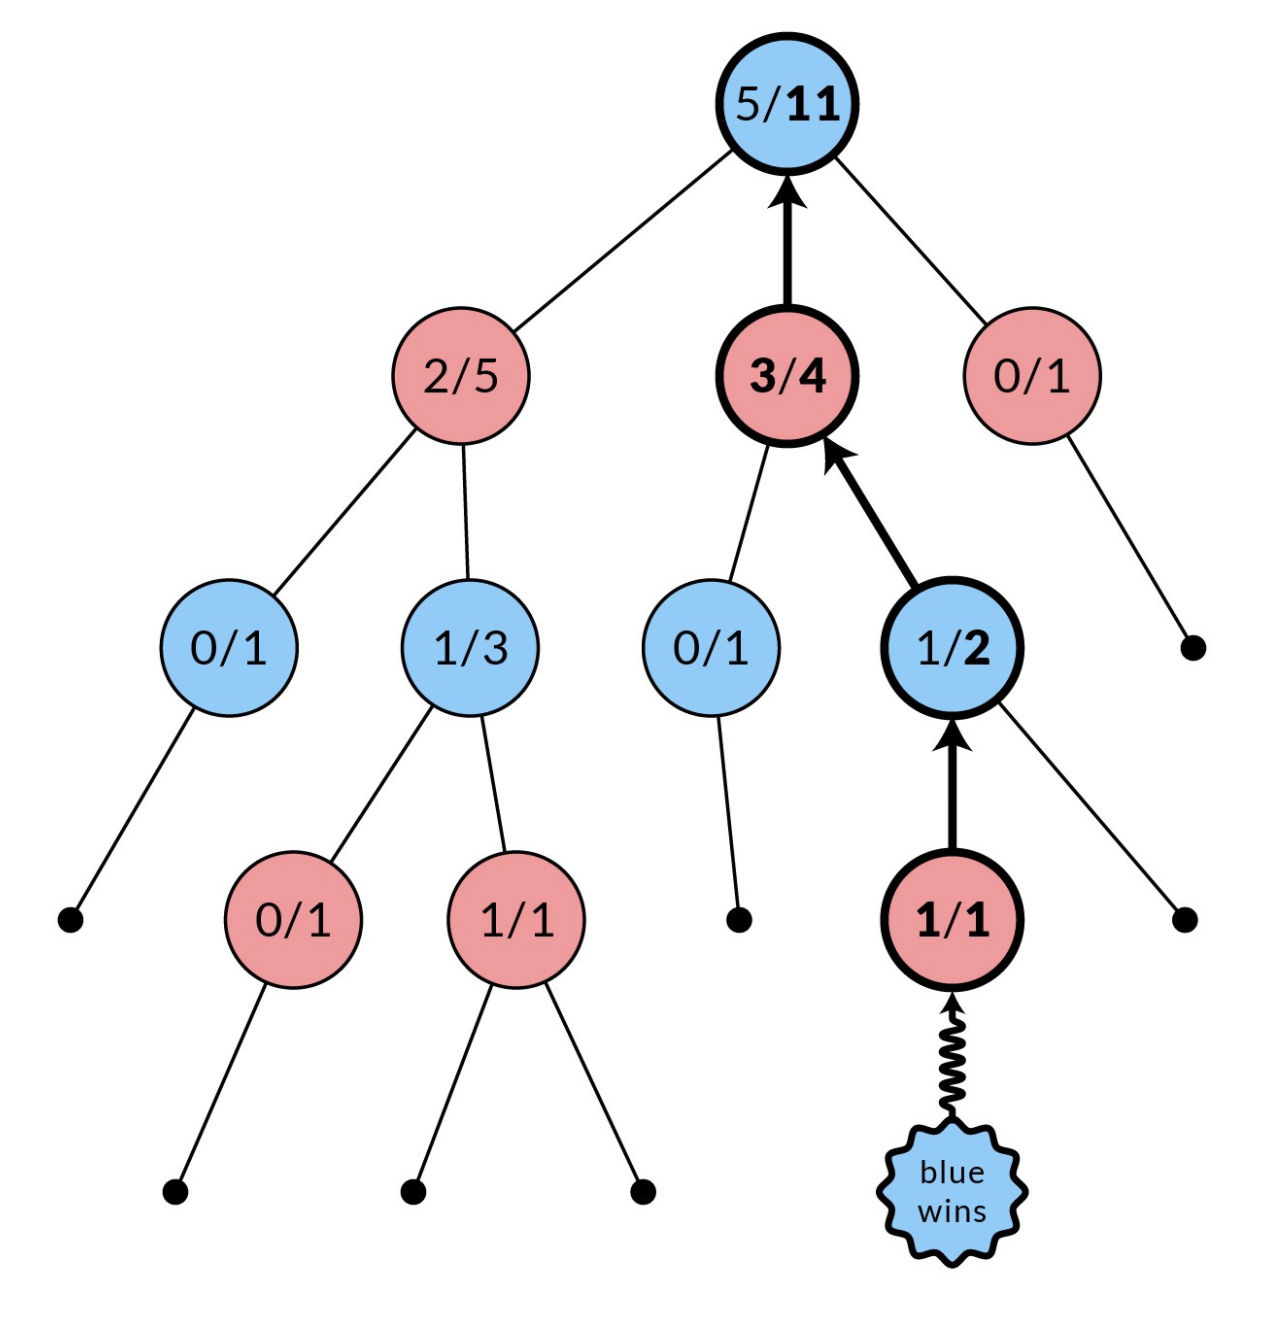
\includegraphics[width=200px,height=200px]{images/mcts_backpropagation.png}





\chapter{AlphaZero}
\section{AlphaZero}
   
   We have looked at minimax, alphabeta pruning and MCTS. They all have nice theoretic guarantees and have been used in many applications. Their main limitation as previously mentioned with minimax is computation. MCTS on its own works fairly well in larger state spaces. There is a limit to this however and being able to solve a game as large as Go will require some modification to the algorithm. We saw how alphabeta pruning cuts out parts of the tree that we know are not adding any information to the decesion making process. Can we accomplish a similar thing with MCTS? The answer is yes, by utilizing deep learning. There have actually been many attempts to improve upon MCTS but fundamentally there are two ways to improve the search. You can either improve the depth of the search or the breadth of the search. In AlphaZero both depth and breadth are improved using neural networks. To give a quick visualization of this process look at the following three figures. They give a picture of a miniature game of Go. You start with an extremely large state space which can be seen in the first figure. You can imagine how large this picture would be if attempting to visualize the entire state space of the full game of Go or Chess. 
   
   \begin{figure}[h!]
       \centering
       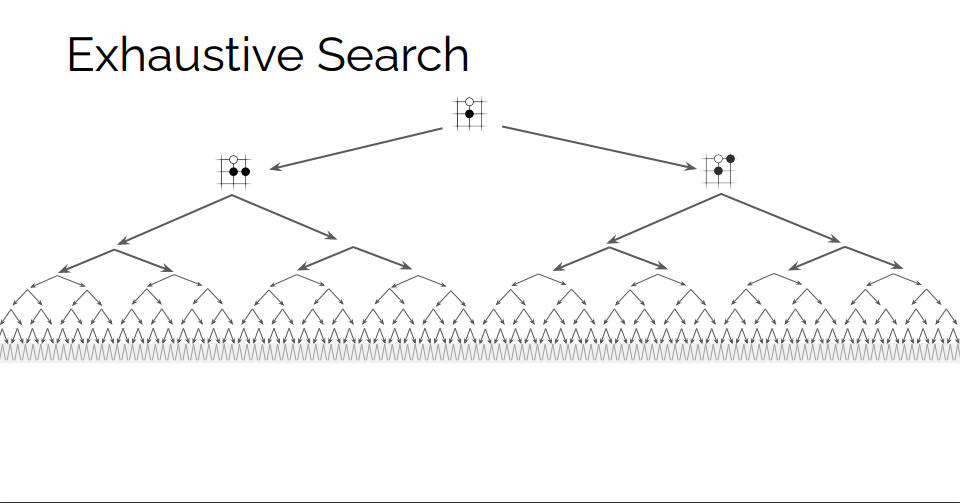
\includegraphics[width=300px,height=200px]{images/julian_exhaustive_search.png}
       \caption{Mini game of go}
       \label{fig:my_label}
   \end{figure}

    \begin{figure}[h!]
       \centering
       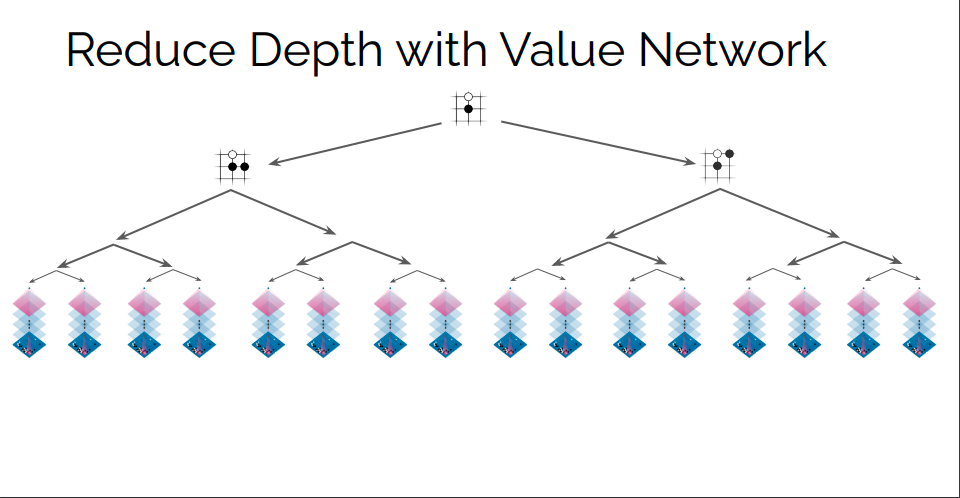
\includegraphics[width=300px,height=200px]{images/julian_reduce_value_network.png}
       \caption{Reduce depth}
       \label{fig:my_label}
   \end{figure}

    \begin{figure}[h!]
       \centering
       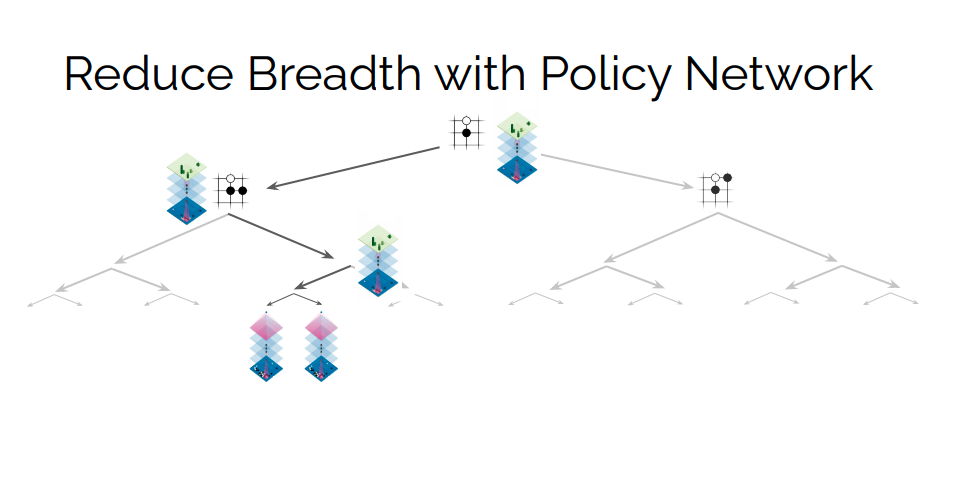
\includegraphics[width=300px,height=200px]{images/julian_reduce_policy_network.png}
       \caption{Reduce breadth}
       \label{fig:my_label}
   \end{figure}
   
   You can see that we have two neural networks a value network and a policy network. The value network (figure 4.2) and the policy network (figure 4.3) work in unison to reduce the state space to something more manageable. The obvious question is how do we actually go about learning both of these networks? 
   
   \section{Expert Data}
   
   Lets first start by actually defining what a value network and a policy network are. First recall that we define the value of a given state as $ v_{\pi}(s) = E_{\pi}[G_{t}| S_{t} = s]$ In the context of a game like Go there are two possible outcomes $ z= \{-1,1\}$. -1 for a loss and +1 for a win. So we can translate the value at a given state to mean a prediction of the outcome $z$ from a given state $s$. A value network is a neural network with weights $ \theta $ s.t. $ v(s,\theta) \approx v_{\pi}(s)$. A policy network on the other hand is a network that helps us with the task of mapping states to actions. Given network weights $\theta$ we have $\pi(a | s, \theta) = Pr\{A_{t} = a | s_{t} = s, \theta_{t} = \theta\}$. So the policy $ \pi $ is actually a distribution over actions. This policy will give you a probability of taking an action from a given state or board position. So this means our policy is stochastic it does not give us a single action to take. 
   
   The approach first introduced by deepmind [2] made use of expert data. We will not go into detail here about their approach but I want to highlight at least the intention of that paper. Assume we have an perfect oracle. That is we have some function $ f(s) \rightarrow v$  that can tell us the true value of being at any possible state? Then we are almost done and can happily do a single pass through the search space to obtain optimal path. At each node starting from the root node of the tree we just take the action that gives us the highest value. We can use our oracle for this by looking at each possible action and seeing which one leads to a state with a higher value. Typically we would have to know something about our opponents policy but here we can plan by acting as both players. We can just assume that our opponent has access to the same oracle and will play perfectly. 
   This can be summed up with the following bellman equation.
   $ a = \underset{a}{argmax} \sum_{s^{'},r} p(s^{'},r | s,a) [r + \gamma f(s^{'})]$. This equation is a form of the bellman optimally equation. Lets break down each part. We are interested in finding the action that gives us the highest return. $ \sum_{s^{'},r} p(s^{'},r | s,a) $ simply means that we are going to look at each of the possible next states assuming we have taken a specific action from our starting state s. This will gives us a probability of each one of those states which we will use to weight the second part of the equation by. The second part $[r + \gamma f(s^{'})]$ is the return that we expect to get
    This assumes you have knowledge of the environment (i.e. you can compute $p(s^{'},r | s,a) $ ). This is an assumption made by MCTS and by the AlphaGo algorithms.
    Since we dont have an oracle we can start thinking about other ways to approximate $f(s)$. Most ways that have been tried historically are taking advantage of expert knowledge. This can be in the form of explicitly hard coding a way to evaluate the value of a state. This has been done in games as complex as chess. You might do something naive like assign a value to each piece. Then count up all the pieces that each side has and assign them a score. 
    
    You could do as more advanced chess programs did and create a database of positions with the actions that were taken by experts at each position. Then you could create a lookup table or another way to approximate a good policy function $ \pi^{*}(s) \rightarrow a $. This second approach is what the first version of AlphaGo did and we will now look at this more deeply. 
    Assume we have created a database of expert games (or other environments). So we have an unordered list of tuples of positions,actions and outcomes. that were played during actual games. That is we have $ (s_{0}, a_{0}, z_{0}), (s_{1}, a_{1}, z_{1}), (s_{2}, a_{2}, z_{2}),..... (s_{n}, a_{n}, z_{n}) = \textbf{D}$ where $s \epsilon \mathbb{R}^{d} , a \epsilon \mathbb{R}^{|A|}$ and as stated before $ z= \{-1,1\}$. There are \textit{n} samples in our database, each state is a vector of size \textit{d} and each action is of size $|A|$ the possible number of actions. We will assume for convenience that d is the dimensions of the environment. If we were playing chess than the board could be represented by a vector of size 8 x 8 = 64. So the set of legal actions will be something $ \leq 64 $ but the state will most likely be $
    \geq d $. For instance we will see that Deepmind used something $ > d$ to represent state. 
     We can sample from the expert $ (s,a) \sim \mathbf{E} $ where $ s $ is some state and $a$ is the action taken by the expert in that state. Sampling from $\mathbb{E}$ will be done uniform randomly s.t. there is no correlation from one sample to the next to help avoid over fitting concerns. 
    We can then employ any of a number of Supervised Learning techniques to learn a policy function $ \hat{f}:s \rightarrow a$ by sampling a large number of data points from $\mathbf{E}$ and minimizing some loss function $L(\hat{f}, \mathbf{E})$. We can do a similar thing to learn a value function by sampling state outcome pairs from the database as well$ (s,z) \sim \mathbf{E} $. The loss function used for the policy network is cross entropy loss and for the value network it is mean squared error. For AlphaGo Fan the first AlphaGo algorithm this was just the seeding step. Once you have your expert networks than you use self-play and MCTS to further improve upon them. There are many details that go into AlphaGo Fan and I encourage the reader to go read the paper if interested [2]. The main thing I want us to think about here is that we are able to use generated data to reduce the depth and breadth of our search. Recall that in MCTS we select actions by 
    
    \begin{equation}
      a = \underset{a}{argmax}(Q(s,a) + U(s,a))
    \end{equation}
    
    In AlphaGo Fan the breadth of the MCTS is reduced by using the policy network to help estimate the uncertainty term U(s,a). 
    
    \begin{equation}
        U(s,a) \propto \frac{P(s,a)}{(1 + N(s,a))}
    \end{equation}
    
    Where P(s,a) comes from the policy network. Reducing the depth is done by replacing the rollout step in MCTS by a rollout network trained on the expert data as well as a value network to help in estimating Q(s,a)
    
    \begin{equation}
        Q(s,a) \propto v(s,\theta)
    \end{equation}
    
    AlphaGo Zero actually makes the architecture much simpler. We will now turn to looking at that and again the reader if interested is encouraged to look at [2] for a more thorough reading of AlphaGo Fan. 
    
    \section{Zero Knowledge}
    
    I first want to highlight some of the main differences between AlphaZero and past implementation like AlphaGo Fan. 
    \begin{itemize}
         \item AlphaGo Zero is trained through self-play only. Starting from random play. There is no expert data used whatsoever. 
         
         \item The input features are only the black and white stones from the board. 
         
         \item It uses a single neural network to represent both the policy and values network. 
         \item It uses a simpler tree search that relies on the single network. It manages to avoid the need for rollouts. 
     
    \end{itemize}

      A big change in accomplishing the above was to move the lookhead search inside the training loop. In AlphaGo Fan the networks were trained first and then those networks were used to run MCTS. In AlphaGo Zero we will see that the network is trained during MCTS. 
    
    The network in short takes in the current board representation and history and outputs a vector of move probabilities and a value.  $ (p,v) = f_{\theta} (s) $. p gives the probability distribution of selecting action a in state s. $ p_{a} = Pr(a|s) $ 
    
    The below diagram gives a nice summary of the training pipeline. Lets look at part $\textbf{a}$ and $\textbf{b}$ separately. 
    
    \begin{figure}[H]
       \centering
       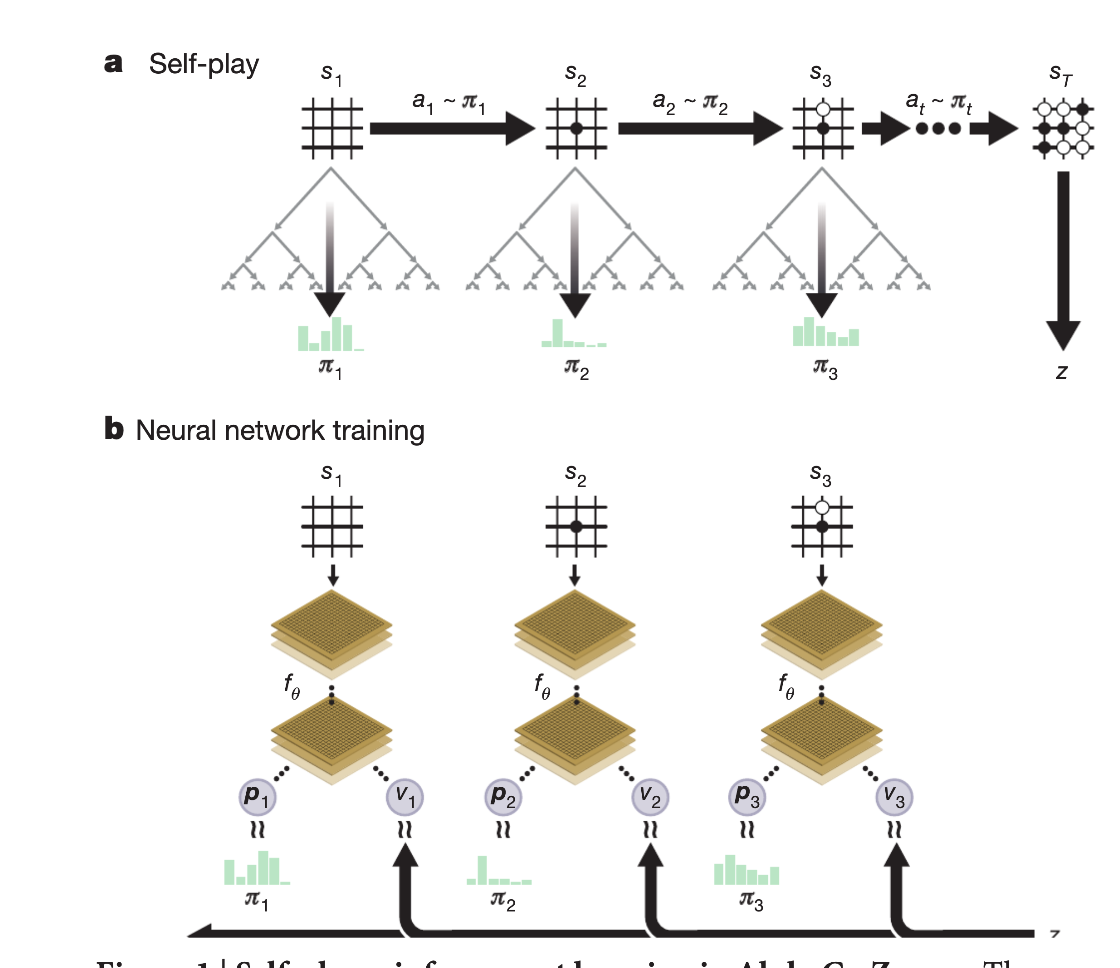
\includegraphics[width=300px,height=150px]{images/alpha_paper_figure_1.png}
       \caption{AlphaZero training pipeline}
       \label{fig:my_label}
   \end{figure}
    
    \textbf{a. Self-play} For each state $s_{t}$ in an episode (game) MCTS is performed and an action is sampled from the move probabilities it outputs. So we can think of MCTS as a function $ \alpha_{\theta} (s_{t}) \rightarrow \pi_{t}$ that takes in the current state and outputs the policy at that point in time. An action is than selected $a_{t} \sim \pi_{t} $ and executed against the environment. We repeat this process until we reach a terminal state and the game ends. We receive a reward from the environment $r_{T} \in (-1,1)$ which we can than use to train the network. 
    
    \textbf{b. Neural Network Training} From part $\textbf{a}$ we have a series of states and outcomes that we can use to improve the network. A single iteration of MCST gives us a series of data points like the following $(s_{1},\pi_{1},z_{1}),(s_{2},\pi_{2},z_{2}),......(s_{T},\pi_{T},z_{T})$ where $z_{t} = \pm r_{T}$. We can now use these to train the network. We will get into the details of the network architecture later but for now it will suffice to know that the loss function is minimized used SGD with the following loss $ l = (z - v)^{2} - \pi^{T} \log p + c ||\theta ||^{2} $. So the loss has three parts. MSE between the networks value prediction and the true outcome, a cross-entropy loss between the distribution output by MCTS and the distribution given by the network, and L2 weight regularization. 
    
    This process can be viewed as an attempt to make the network more closely resemble the outcome that is being given by MCTS. In this way MCTS acts as the guide for continual improvement. The search probabilities $\pi$ are generally going to give better action selections than what the current network advises. So MCTS acts as policy improvement operator. Also the outcome of games $\textbf{z}$ were obtained using MCTS and so they can be viewed as a policy evaluation operator. If you have a way to both improve a policy and evaluate the new policy than you have a way to perform policy iteration.
    
    Ok now we will dig into the MCTS a bit more and then take a look at how the network is trained after that. The below diagram taken from the paper displays each of the steps. Lets go through each
    
    \begin{figure}[H]
       \centering
       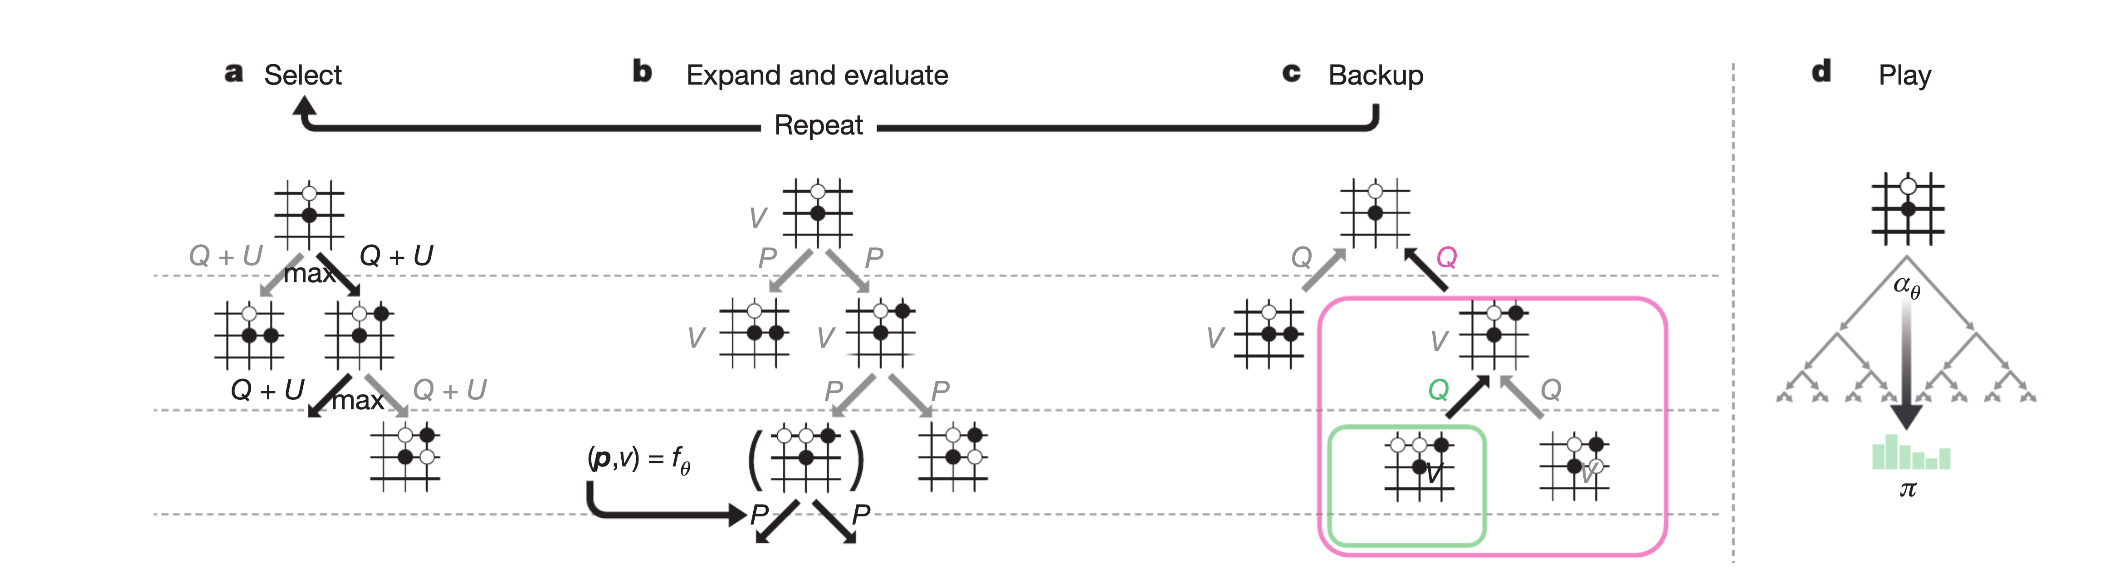
\includegraphics[width=300px,height=150px]{images/alpha_paper_figure_2.png}
       \caption{AlphaZero training pipeline}
       \label{fig:my_label}
   \end{figure}
   
   \textbf{Overview} Each \textbf{edge} in the tree stores a set of statistics. For all legal actions from a given node $ a \in A(s) $ the set $\{ N(s,a),W(s,a),Q(s,a),P(s,a) \}$ is stored. $N(s,a)$ is the visit count, $W(s,a)$ it the total action-value, $Q(s,a)$ is the mean action value, and $P(s,a)$ is the prior probability given by the network for the (s,a) edge. 
       
   The algorithm starts at the root node of the tree and then repeats steps (a-c) a given number of times. After these simulations are complete an action is selected based off of the accumulated statistics. The current node of the tree is moved to the next node based off of the action that was selected. The process is repeated for the new node until a terminal node is reached. The results are stored in order to train the network and the process is repeated from the root node once again. 
   
   \textbf{Selection} As with all the versions of MCTS we have looked at so far selections are made by taking actions by taking the max of a value term plus an upper confidence bound term. $\underset{a}{argmax} (Q(s,a) + U(s,a))$ In this case both terms come from the network. $U(s,a) \propto P(s,a) / (1 + N(s,a)) $ where $P(s,a) $ is given by the probability distribution over action $\textbf{p}$ from the network. $Q(s,a) = \frac{1}{N(s,a)}\sum_{s^{'}|s,a \rightarrow s^{'}}V(s^{'})$ So $Q(s,a)$ is just the mean over the value of the next states
   
   \textbf{Expand and evaluate} Once a leaf node is reached the leaf node is expanded and the leaf node is evaluated by the neural network. $ (P(s_{L}),V(s_{L})) = f_{\theta}(s) $ Then each edge is initialized with the following $ N(s,a) = 0,W(s,a) = 0,Q(s,a) = 0,P(s,a) = p_{a} $. The value of the leaf node $\textbb{v}$ is backed up. 
   
   \textbf{Backup} For each step that was visited from step (a,b) the statistics for each of the visited edges are
   updated. $N(s_{t},a_{t}) += 1$ , $W(s_{t},a_{t}) += \textbb{v} $, and $Q(s_{t},a_{t})=\frac{(s_{t},a_{t})}{N(s_{t},a_{t})} $
   
   \textbf{Play} After a given number of iterations from the current node an action is selected and executed against the environment. The policy that is output by MCTS is given by the following formula. $\pi(a|s) = \frac{N(s,a)^{\frac{1}{\tau}}}{\sum_{b}N(s,b)^{\frac{1}{\tau}}}$
       
   $\tau$ is called a temperature parameter that controls the level of exploration. For each time step the statistics in the tree below the node of interest are retained. The statistics above are discarded and will be repopulated in the future if that node is revisited.
   
   We will now turn to focusing on the deep learning aspect of the algorithm. We have already discussed how data is collected and what loss function is used while training. Lets start with what the input looked like and than look at the architecture of the network itself. The input to the NN is a 19x19x17 image stack. There are 8 images for the current player and 8 for opponent and The final layer being a representation of who is to play. So the feature input at time $t$ is $s_{t} = [X_{t},Y_{t},X_{t - 1},Y_{t -1},... X_{t-7},Y_{t-7},C]$. Here $X_{t}$ is a 19 x 19 frame of ones and zeros. The ones representing the position of all of blacks stones at time t. Likewise $Y_{t}$ is the same except all ones for whites stones and zero elsewhere. C here is a 19 x 19 frame representing the player to act at time $t$. Its a frame of all ones if it is black to act and all zeros if it is white to act. 
   
   As mentioned previously the network used in AlphaZero is a two headed network. There is a single convolutional layer that processes the input followed by 39 residual blocks. Then the policy head consists of a convolutional layer, batch norm, relu and a fully connected layer. The value head is similar but with an extra convolutional layer and the output contains a $tanh$ function which works well for two player games since that constrains values to be between -1 and 1. They found that residual blocks performed better than convolutional layers. I think for understanding the core concepts it is not necessary to fully understand how all of the pieces of the deep learning architecture work. In the next section we will look at what it takes to build a smaller example of the architecture on your own. We will also look at some experiments that I ran using the game of ticatactoe and connect4 to help clarify some of the concepts discussed so far. 
    

\chapter{Experiments}
\section{Empirical Finding}

\subsection{Coding AlphaZero}

It is one thing to read a paper and understand something at a high level and it is another to actually implement the concept described. Here I will discuss my own efforts and struggles in implementing AlphaZero on smaller environments. I think it good to clear up some terminology confusion that can arise. When I say that I implemented AlphaZero and what most people mean when they talk about AlphaZero is the general concepts used to solve the game of Go. So this means that the specific hyperparameters or network architecture is not necessary implement your own version on a different environment. I will recap here what those core concepts of AlphaZero are. 

\begin{algorithm}[H]
\SetKwFunction{FSelfPlay}{SelfPlay}
\SetKwFunction{FTrainNetwork}{TrainNetwork}
\SetKwFunction{FEval}{Eval}
\SetAlgoLined
 init Network\;
 init ReplayBuffer;
 
 \For{iter in iters}{
  
  run \FSelfPlay
  
  run \FTrainNetwork
  
  run \FEval
  
 }
 \caption{AlphaZero Core}
  
\end{algorithm}

In Algorithm one above you can see that the algorithm can actually be condensed to a small number of parts. Each one of those parts has a lot going on but it helps to have a high level understanding of the algorithm before getting into the details. Let go through each piece. The first thing that happens is the network is randomly initialized. We refer to both policy and value networks as a single network. The algorithm is run for a predefined number of iterations. You could also have a stopping criterion if you wanted based on performance. For each iteration of the algorithm we do three main things. Self-play, network training and evaluation. The self play step is what generates the data for our network to train on. We play some predetermined number of games against ourselves. The results of those games are saved off for training the network. Playing against yourself here means that the role of player 1 and player 2 is assumed by the same AlphaZero agent and therefore the same network. Training the network means random sampling a batch of data from the replay buffer some number of epochs. The network is updated each epoch using backpropagation to minimize the loss function previously mentioned.  

\begin{equation}
    l = (v - z)^{2} - \pi^{T} \log{\hat{\pi_{\theta}}} + c||\theta||^{2}
\end{equation}

The final step is the evaluation step. In the AlphaGo Zero paper this was performed by keeping track of a best network. You keep a best network in memory and then after every time you update the current network you have your newly updated network play against the current best. If the current network beats the current best by a certain threshold then the current network is now set the best network otherwise the current network is discarded. So in this scheme you dont actually keep your updated network until it is able to beat the previous best version. In my own implementation I found that this hurt performance and I opted to continually update the network each iteration. This is actually what they do in their follow up paper AlphaZero [3]. Lets look at self play in a little more detail. 


\begin{algorithm}[H]
\SetKwFunction{FSelfPlay}{SelfPlay}
\SetKwFunction{FMCTS}{MCTS}
\SetAlgoLined
\SetKwProg{Fn}{Def}{:}{}
 \Fn{\FSelfPlay{$Agent$,$NumberGames$}}{
    
    \For{game in Games}{
        
        reset Tree;
        
        reset Env; 
        
        \While{True}{
            
            $s_{t} \sim Env$ 
            
            $a \sim MCTS(s)$
            
            $s_{t}, a, s_{t + 1}, r, done \sim Env.next(s)$
            
            $Agent.StoreMemory(s_{t},a,r)$
            
            \If{done}{
                break;
            
            }
            
        \EndWhile
      }
    }
}
\end{algorithm}


A few things of note in the SelfPlay algorithm above. The first is that at the beginning of each game the tree is being reset. When the agent runs MCTS to select an action all of the statistics above the current node in the tree are forgotten about. It is possible to have different criterion for how often you reset the statisics in the tre but the idea is that old statistics were generated by an old network and therefore not as reliable. We will discuss specifics of MCTS and the different hyper parameters used later. We next give a brief look at the network training step. 

\begin{algorithm}[H]
\SetKwFunction{FTrainNetwork}{TrainNetwork}
\SetAlgoLined
\SetKwProg{Fn}{Def}{:}{}
 \Fn{\FTrainNetwork{$Agent$,$Epochs$}}{
    
    \For{epoch in Epochs}{
        $ s, \hat{\pi}, z \sim Agent.Memory$ \Command{Sample data from replay buffer that was created during self play}
        
        $ (\pi_{\theta} , v ) \sim Agent.NN(s) $ \Command{Pass s through the network}
        
        $ l = (z - v)^{2} + \pi^{T} \log{\hat{\pi_{\theta}}} + c||\theta||^{2}$
        
        $ \theta_{t} = \theta_{t -1} - \alpha \frac{\partial l}{\partial \theta}$
    }
}
\end{algorithm}


\subsection{TicTacToe Experiments}

Now that we have a reasonably good idea of what the high level logic looks I believe you should have a good idea of how the algorithm works. Lets look at a few experiments to try and get a better feel for how the algorithm works in practice. These first few set of experiments we will be running AlphaZero on the game of tictactoe. Tictactoe is played on a 3x3 grid. The players place pieces onto the grid with goal of connecting 3 in a row. You can connect 3 in row horizontally, vertically or diagonally. The game is nice because it is small enough that we can actually find optimal solutions. I will use the same neural network architecture for all of the experiments that follow. 

\textbf{NN Architecture}
\begin{itemize}
    \item Convolutional Layer with padding + BatchNorm
    \item Convolutional Layer with padding + BatchNorm
    \item Convolutional Layer + BatchNorm
    \item policy head is just a single fully connected layer with a log softmax as an activation function
    \item value head is also a fully connected layer but with $tanh$ as the activation function
\end{itemize}

You can see that there are no residual connections used here. This could certainly be added for improved performance but the goal here was to get use something small but still had some of the properties of what a larger application would need.  I did for instance use just a simple Neural architecture that only had fully connected layers and the performance seemed to suffer quite noticeably. If the reader is interested in attempting different architectures please go the github page linked to in the abstract. It is quite easy to change if desired. I used pytorch for building the network and for training the network. Pytorch is an open source machine learning framework that is supposed to be used for "research to production". The VikingZero codebase does not depend heavily on the framework used and would not take much effort to swap out pytorch for tensorflow or something else. 

In the AlphaGo Zero paper the input to the network is an actual stack of frames. This is nice because it automatically encodes some temporal knowledge. In the VikingZero implementation I dont look back any time steps. So the input is a single frame for each player and then a layer representing whose turn it is. So here is what that looks like. 

\begin{figure}[H]
       \centering
       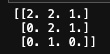
\includegraphics[width=100px,height=100px]{experiments/demo_board_1.png}
       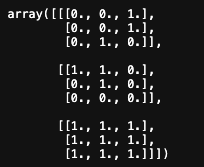
\includegraphics[width=100px,height=100px]{experiments/transform_demo_board.png}
       \caption{Left Figure is a tictactoe board. Figure on the right is the transformed version }
       \label{fig:my_label}
\end{figure}

Now lets discuss the relevant hyper parameters that require tuning. In the AlphaGo Zero paper they used Bayesian hyper parameter optimization to tune their network. I did not have that luxury and so I tuned the network "by hand". That basically just means you start with a best guess at an architecture, run an experiment, view the outcome, change a single hyperparameter and repeat. AlphaZero has a lot of hyperparameters which makes tuning it rather cumbersome. The list below is quite long but I hope that it helps demonstrate that it is not as simple as aiming the algorithm at a problem and hitting go and expecting good results. 

\textbf{Exploration parameters}
These are the hyper-parameters that changed how much exploration was done throughout training. First recall that actions during MCTS are selected by the following equation. 

\begin{equation}
    a_{t} = \underset{a}{argmax}(Q(s_{t},a) + U(s_{t},a))
\end{equation}

\begin{equation}
    U(s_{t},a) = c_{puct}P(s,a) \frac{\sqrt{\sum_{b}N(s,b)}}{1 + N(s,a)}
\end{equation}

More weight is given to $U(s,a)$ when N(s,a) is small relative to $\sum_{b}N(s,b)$. That is when the action $a$ associated with node $s$ has not been visited often relative to the other actions. More weight is given to $U(s,a)$ when the policy network $P(s,a)$ is larger. That means that the more opinionated the policy network becomes more likely it is to select that action during MCTS. This is a potential area for over fitting. 

\begin{itemize}
    \item \textbf{$c_{puct}$} This simply weights $U(s,a)$. Increasing $c_{puct}$ increases exploration. I found that the commonly used $\sqrt{2}$ was best. 
    \item \textbf{dirchlet noise}. This simply adds extra noise to the root of the search tree during MCTS and encourages additional exploration. This is \textbf{Not} used on any other nodes of tree other than the current root. Actions are then selected by
    $P(s,a) = (1 - \epsilon)p_{a} + \epsilon \eta_{a}$ where $\eta \sim Dir(\alpha_{d}$
    In my experiments I found that $epsilon = 0.1$ and $\alpha_{d}=0.03$ (same as paper) was best. Epsilon > 0.1 tended to cause too much variability in the action selected by MCTS resuliting in large variability during network training. 
    \item $\tau $ threshold. In the AlphaGo Zero paper actions against the actual environment are selected according to $\pi(a|s) = \frac{N(s,a)^{\frac{1}{\tau}}}{\sum_{b}N(s,b)^{\frac{1}{\tau}}}$ for a given number actions. After that given number of actions the action with the highest probability is selected. This translate into setting $\tau = 1$ during the beginning of play and then setting $tau -> 0$ once the agents has taken more actions than the threshold. I found that having the threshold = 3 in tictactoe worked well. 
\end{itemize}

\textbf{Network Parameters}

Now lets look at the hyperparameters w.r.t network training. 

\begin{itemize}
    \item \textbf{Optimizer}. Throughout these experiments I use the Adam optimizer provided by pytorch. In the paper they use SGD with momentum. I found that Adam outperformed for all of my experiments. 
    \item \textbf{lr} learning rate. The learning rate that I used was 0.001
    \item \textbf{Batch size}. This is how many samples are randomly sampled for each epoch of training. I used a batch size of 32 but found that sizes between [16,64] gave similar results. 
    \item \textbf{epochs}. See the \textbf{TrainNetwork} function above. Running 25 epochs worked best for me but this seemed like a bit large for a game like tictactoe but thats what worked best for me. 
    \item \textbf{Maxmemsize}. How much memory you allow to be kept in the replay buffer can have a significant affect on performance. For instance I kept a max size of 20k for a long time and then realized that this kept too much old data and did not allow the network to correctly capitalize on a newly "found" strategies. 
    
\end{itemize}

\textbf{More Parameters..}

\begin{itemize}
    \item \textbf{number of sims}. This refers to the number of times you run an iteration of MCTS from your root node. I found that running 25 simulations worked well. It was enough simulations that it gave your policy network a good target. Remember that running MCTS outputs $\hat{\pi}$ with the policy network tries to approximate. So if you dont run enough simulations $\hat{\pi}$ wont be very good. On the other hand running a lot is very costly computationally. So ideally you want the least number that is necessary to continuously be able to improve your policy network. 
    \item \textbf{number of games}. The number of games that you play (see Def SelfPlay) per iteration changes how much data that you end up generating. Generally in deep learning a lot of data is required. It is no different in this setting. If you dont play enough games than you wont have enough data to train on but if you play too many games you can end up overfitting to the current network. For tictactoe I found that playing 30 games was best. 
\end{itemize}

\textbf{Evaluation}

For evaluating the performance I used a few different metrics. The first metric was to play the agent vs a minimax agent and track the total score over iterations. For tictactoe this allowed me to get a comparison against an optimal agent. For Connect4 a minimax or full depth alphabeta agent was too slow. I used a depth limited alphabeta agent. Please see the Search section for a discussion on the alphabeta algorithm. The loss values for the policy and value networks are tracked every iteration. This is mostly to ensure the algorithm is actually learning. As we will see having a small error does not translate to winning. Another metric I used exclusively for the tictactoe experiments was an optimal play lookup. I used a minimax agent to look at every possible state and create a dictionary lookup of state --> action. The size of the dictionary is 4520. This ignores illegal positions and positions where the board is full since in that case there is no action to look at. To compare against the current agent I do an exhaustive comparison of the agents max actions vs the minimax action. I then report the mean score. This is an expensive test and so running it every iteration is not feasible but it gives a thorough look at the agents performance. 


\subsection{TicTacToe Experiments}

In these series of experiments we will show our best models performance and the hyperparameters used. We will then do a comparison vs other settings and do a side by side comparison. 

\textbf{Base model settings}

\begin{multicols}{2}

\begin{itemize}
    \item Batch size: 32
    \item $c_{puct}: 1.41$
    \item dirchlet noise: 0.03
    \item epochs: 25
    \item epsilon: 0.1

\end{itemize}

\begin{itemize}
    \item learning rate: 0.001
    \item max memory size: 5000
    \item number simulations: 25
    \item tau threshold: 3
    \item episodes: 300
    \item number training games: 30
\end{itemize}

\end{multicols}


\begin{figure}[H]
       \centering
       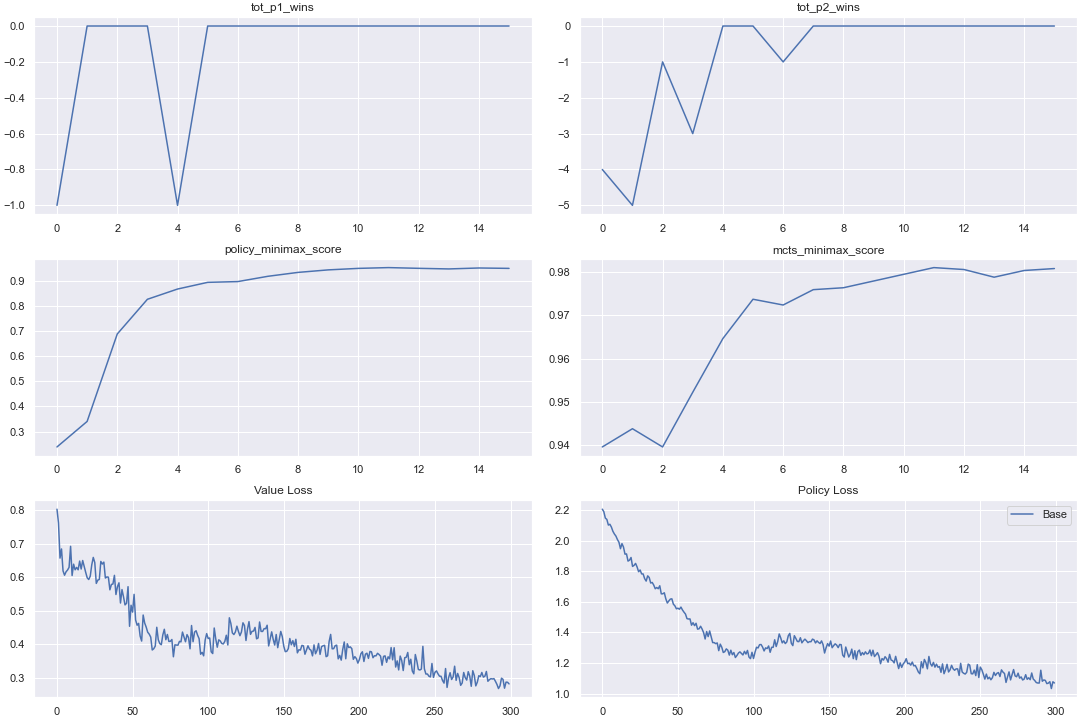
\includegraphics[width=400px,height=400px]{experiments/base_model.png}
       \caption{Base Case experiment}
       \label{fig:my_label}
\end{figure}

For the base case experiment looking at the figures left to right. tot\_p1\_wins is the total score out of 5 games. The agent gets a +1 for a win a -1 for a loss and 0 for a draw. Since minimax plays perfectly the best the agent can hope to do is get a score of 0. We can see that this is achieved fairly quickly from the perspective of player 1. From the perspective of player 2 we can see from the second figure that eventually the agent reaches a poit of always getting a draw vs minimax but is much more volitile at the beginning of training. The 




\textbf{Experiment 1}

In our first comparison we will look at the affect of the tau threshold on performance. Lowering the threshold equates to less variability in the data seen by the network. This in turn leads to less exploration in future iterations of training as the network learns to more quickly prefer those higher probability actions. This can lead to over fitting if there is not enough exploration in the MCTS portion of the algorithm. Below we show our base model in comparison with a model that has tau = 1 instead of 3. In this case there does seem to be over-fitting happening. We see from the loss graphs that the network quickly goes to having almost 0 loss. This would be good if we were doing supervised learning but here in the RL setting that does not always translate to a good outcome since we are generating our own dataset from interacting with the environment. The most striking difference I think here is looking at the "mcts\_minimax\_score". This shows how the tau=1 model quickly hits max performance and plateaus. We can also see that in performance vs minimax the tau=1 model was bouncing around quite a bit more. 

\begin{figure}[H]
       \centering
       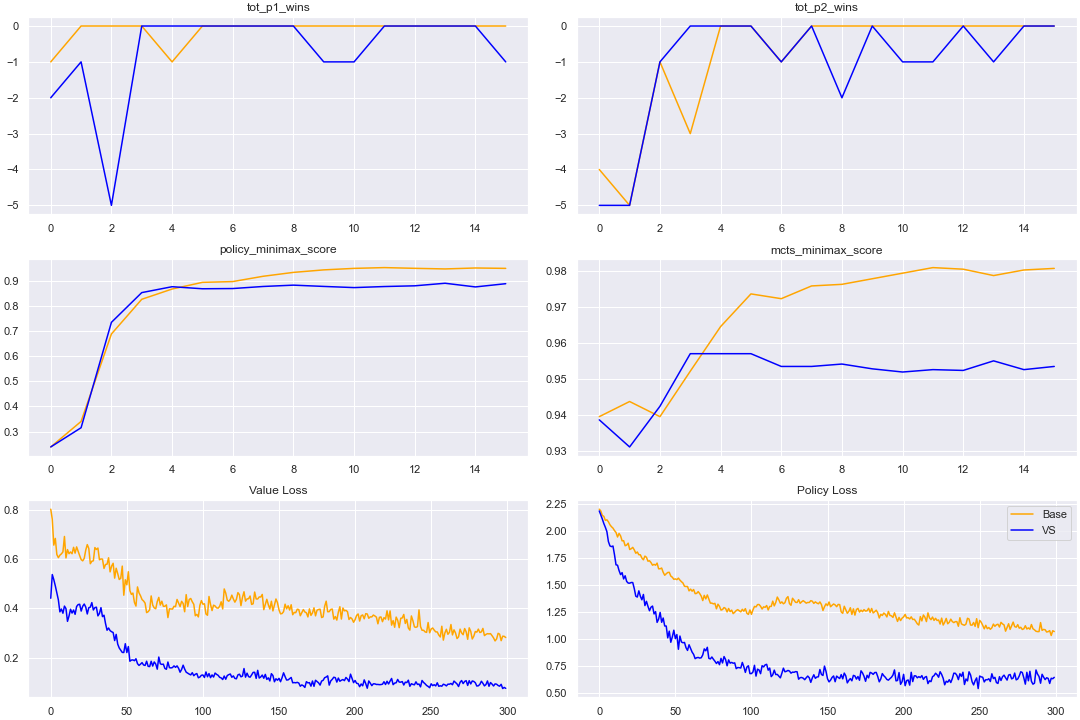
\includegraphics[width=400px,height=300px]{experiments/base_vs_t=2.png}
       \caption{Base Case experiment}
       \label{fig:my_label}
\end{figure}




\textbf{Experiment 2}

In this second comparison we will look at the affect of increasing the amount of noise during search by setting epsilon = 0.2. Recall that this increased noise happens only at the root of the search tree during MCTS. It seems that this model actually performs slightly better than our base model in the "mcts\_minimax\_score" but quite a bit more variability in its performance vs minimax. Not suprisingly the value and policy loss values are much higher. This is not surprising since we have a lot of variability in our training data. This highlights the point that increased exploration even if it comes at the cost of worse network performance might be worth it. 

\begin{figure}[H]
       \centering
       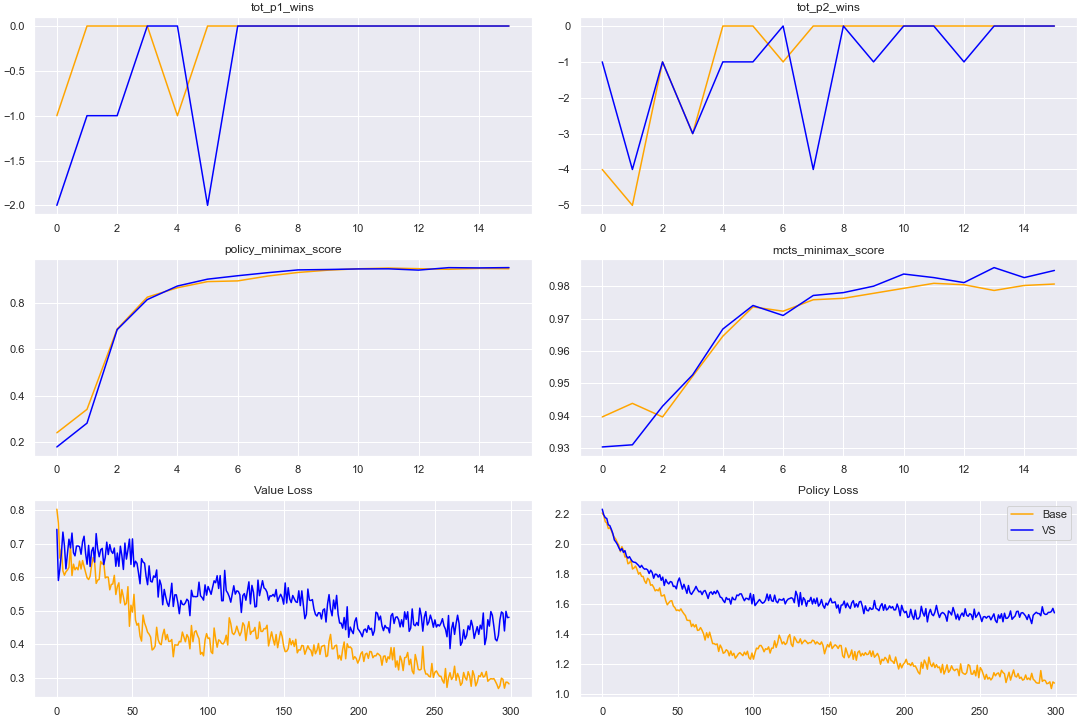
\includegraphics[width=400px,height=300px]{experiments/base_vs_eps=0_2.png}
       \caption{Base vs epsilon = 0.2}
       \label{fig:my_label}
\end{figure}



\textbf{Experiment 3}

In this third comparison we will look at the affect of decreasing the number of simulations performed during search. This really hurts performance more than any other metric. This was suprising to me given such a small environment such as tictactoe. It appears that even in non complex domains that a minimum amount of exploration is required and 15 simulations was not enough to both explore and exploit the better paths.  

\begin{figure}[H]
       \centering
       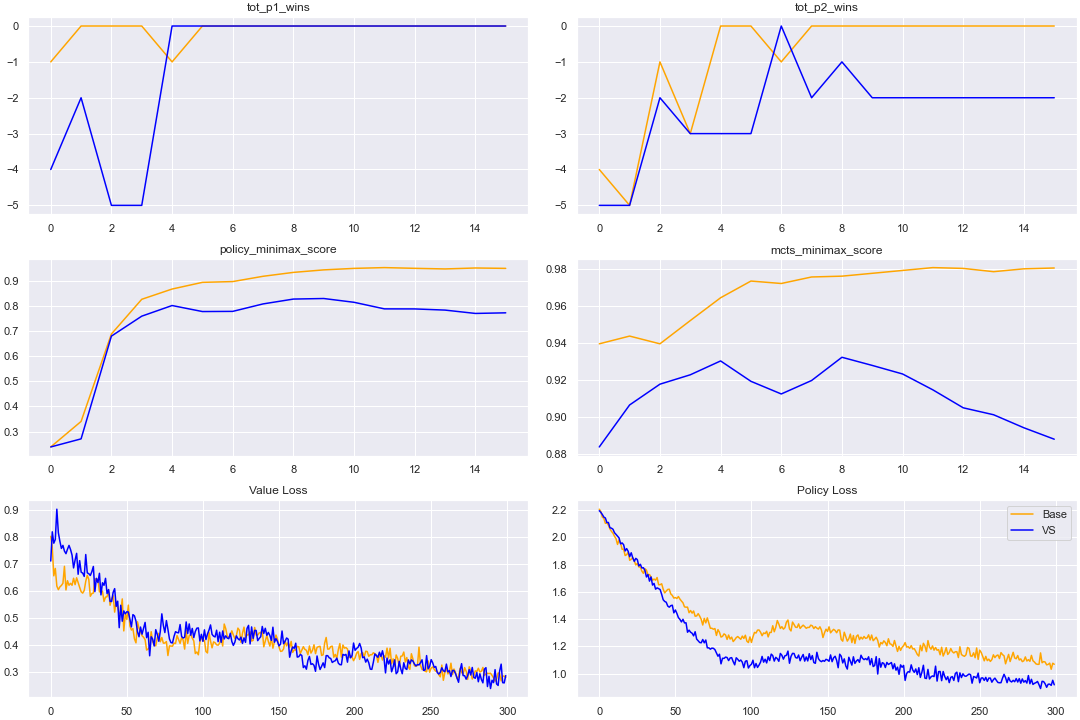
\includegraphics[width=400px,height=300px]{experiments/base_vs_nsim=15.png}
       \caption{Base vs nsim = 15}
       \label{fig:my_label}
\end{figure}


\textbf{Experiment 4}

In this fourth comparison we will look at the affect of increasing the number of games played per episode as well as increasing the maximum memory size. Here we set the max memory to 20000 and we play 50 games per iteration. This of course generates much more data than previous and allows us to keep more in memory. This should help to prevent over-fitting. Playing more games equates to seeing more board positions especially when the network is less certian about withc is best. Here we found that we did not increase performance and might have even hurt performance slightly. From the experiments that we ran it seemed however that this is something that will require a good amount of tuning. Large domains of course will require much more training data and will require you to hold on to older data for longer as well. 

\begin{figure}[H]
       \centering
       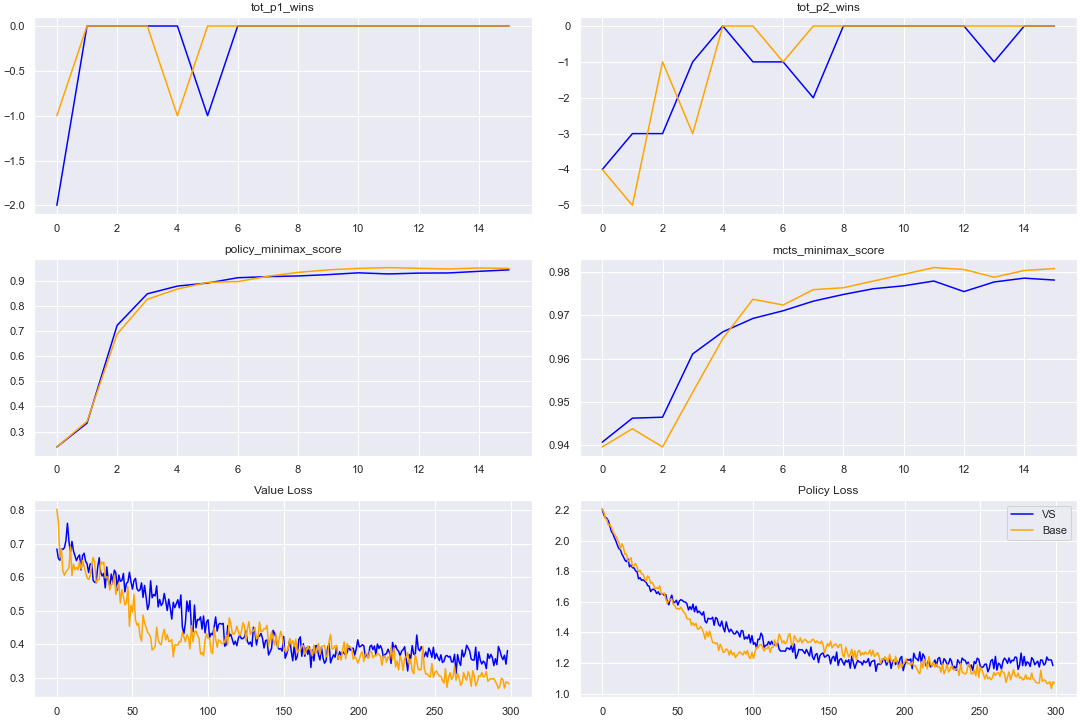
\includegraphics[width=400px,height=300px]{experiments/base_vs_maxmem.png}
       \caption{Base Case vs maxmem size}
       \label{fig:my_label}
\end{figure}


\textbf{Experiment 5}

Lets now look at an interesting experiment in which we increase the number of epochs the network runs. In the base case we run 25 and so what should doubling them do? My first guess was that it was going to over-fit and I am sure there is some high number of epoochs that you could run that would cause that to happen but I found that doubling the number of epochs actually seemed to help performance. The player 1 performance vs minimax immediately goes to optimal and stays there for the rest of training. The policy and mcts minimax scores are both better as well. 

\begin{figure}[H]
       \centering
       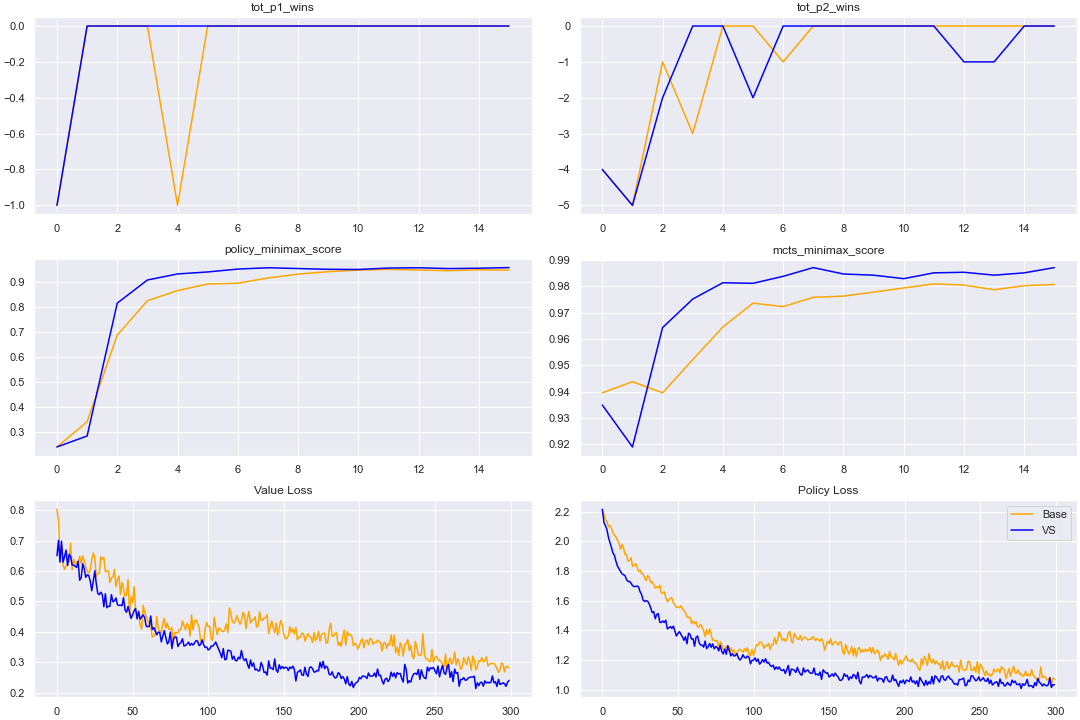
\includegraphics[width=400px,height=300px]{experiments/base_vs_epochs=50.png}
       \caption{Base Case vs Epochs =50}
       \label{fig:my_label}
\end{figure}


\subsection{Connect4 Experiments}

Lets now look at how our implementation does on the game of connect4. In these tests we were not able to use the minimax scores that we could do with tictactoe since we needed a dictionary action lookup over the full state space. So we will drop those tests. The game of connect 4 is the same as tictactoe expect the goal is to get 4 in a row instead of 3. It is played on a 6 x 7 board. 

\textbf{Parameters}

\begin{multicols}{2}

\begin{itemize}
    \item Batch size: 64
    \item max memory size: 20000
    \item number simulations: 35

\end{itemize}

\begin{itemize}
    \item tau threshold: 10
    \item number training games: 20
\end{itemize}

\end{multicols}

\begin{figure}[H]
       \centering
       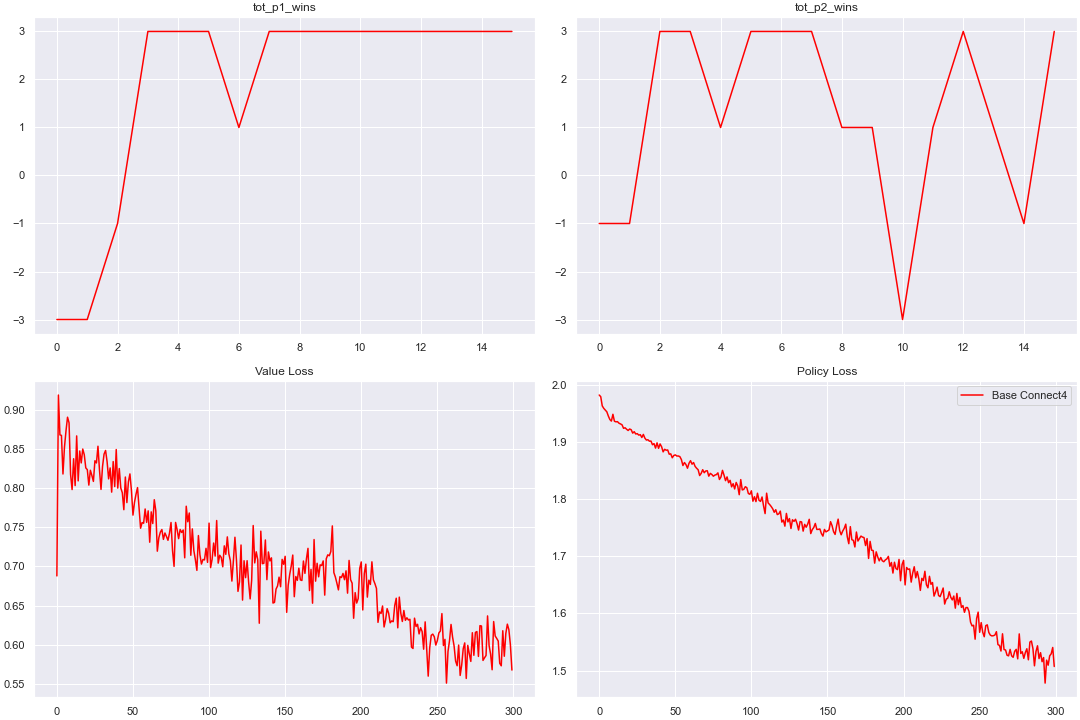
\includegraphics[width=400px,height=300px]{experiments/base_connect4.png}
       \caption{Base Case vs Epochs =50}
       \label{fig:my_label}
\end{figure}

\chapter{Other Work}

In this section we will discuss some of the work that has come out since AlphaZero. There have been a number of improvements as well as an increased theoretical understanding. This will not be an exhaustive treatment of the work and is only intended to give the reader a taste of what is out there in the hopes that will make further pursuit of these topics easier. It will not be exhaustive in depth or in breadth. There is more work being produce seemingly all the time that builds on top of what we have discussed in this paper. 

\section{MuZero}

Recall that while training a AlphaGo algorithm you need a model of the environment. In order to perform MCTS you have to have an accurate model of the environment that is capable of giving you the next state given a current state and action. The environment also needs to tell you when the game has ended and what the associated reward is. This is a barrier for being able to apply the concepts learned in ALphaGo to other domains. In 2019 Deepmind released a paper \cite{muzero} that helped to address these issues. The algorithm has many similarities to AlphaZero and so lets look at where it differs. MuZero performs MCTS in a latent space with a learned model. That is as they are performing each step of MCTS in a state space that is not directly representative of an actual state in the environment. Let look at a figure of this to see what I mean. 

\begin{figure}[H]
       \centering
       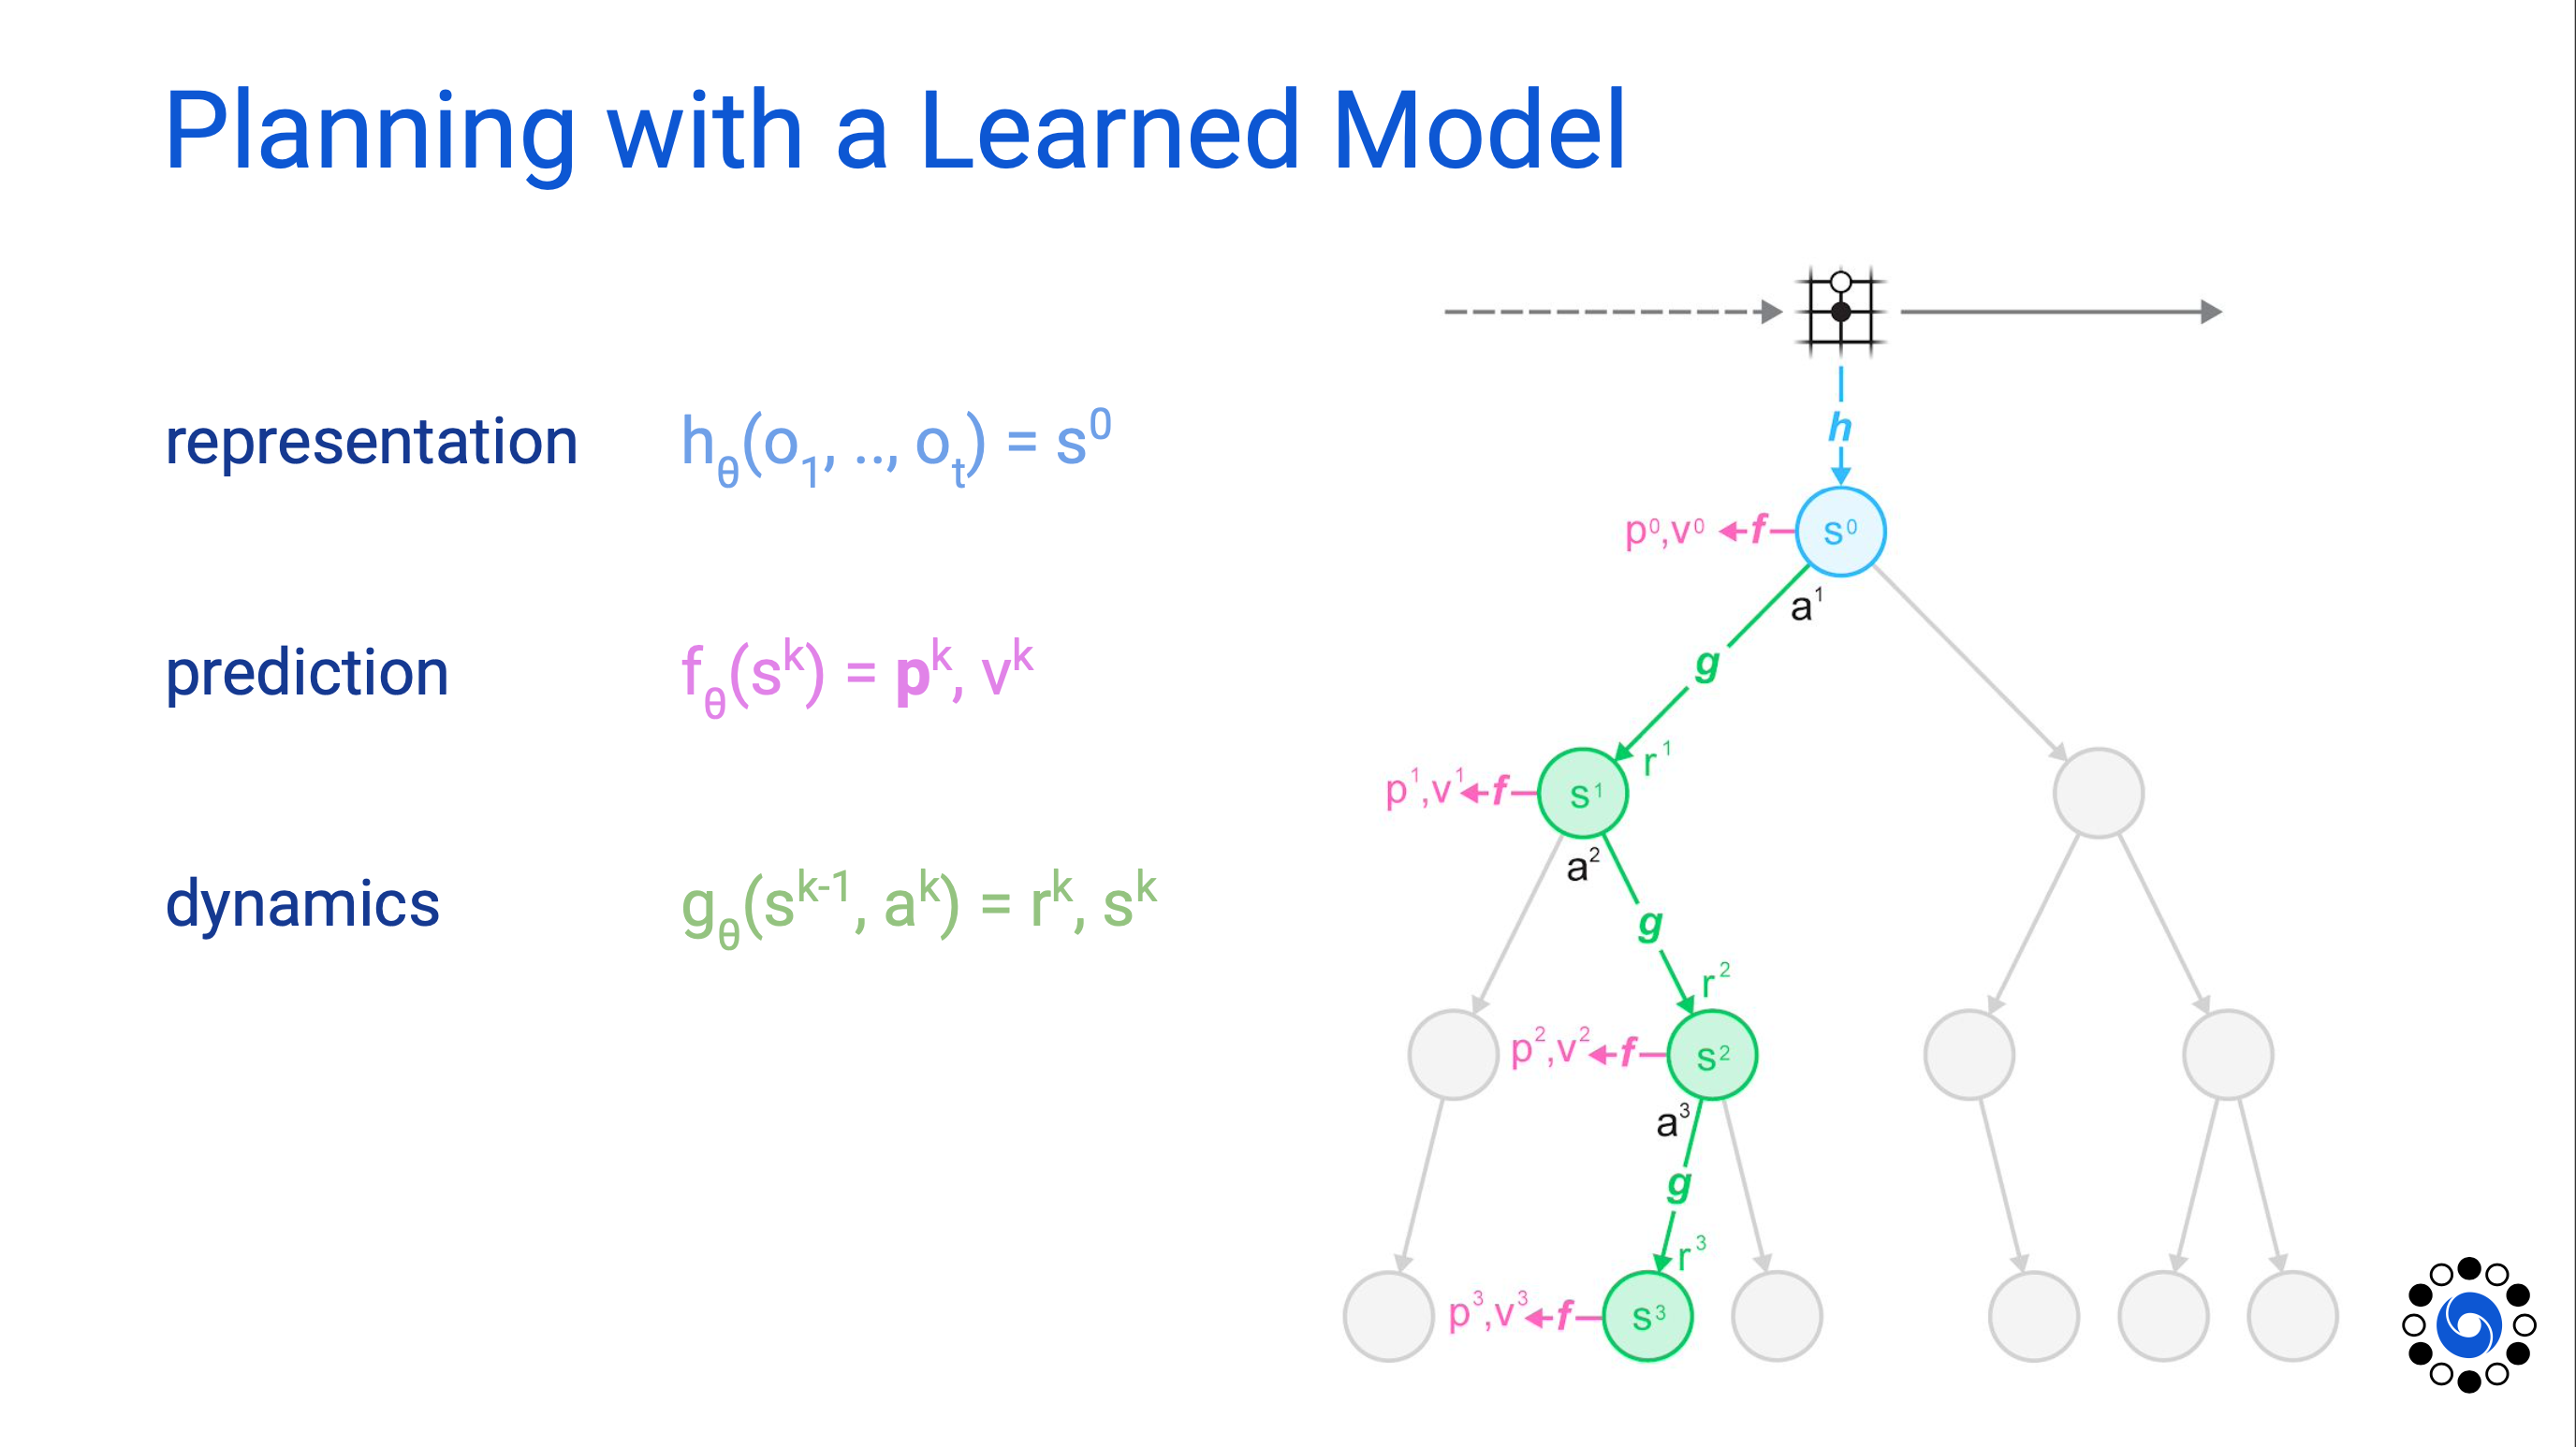
\includegraphics[width=400px,height=200px]{images/muzero_learned_model.png}
       \caption{Planning in MuZero}
       \label{fig:my_label}
\end{figure}

The current state of the environment is used for the root node as usual except now there is a \textbf{representation} network that takes the environment state and produces a vector representation of that state in a latent space. From this new space you need to run all the normal MCTS except without a model. This is achieved by learning a dynamics model that sits in place of the true environment. The interesting thing is that this dynamics model is not learned by attempting to make it be able to model the true environment more and more accurately which is the standard approach. Here the dynamics model is learned so as to maximize reward (more to come on reward). The idea is that in some cases it might not be necessary and even detrimental to plan with the true model. From the figure you can see that the dynamics function takes in a state action pair and produces the next state and reward. This means that they are also learning a representation for reward. This has the flexibility of potentially learning intermediate reward states. There is still a network that outputs a policy and a value from a given state represented in the figure as the \textbf{prediction} $f_\theta$. Since there is no environment to tell the search when its hit a leaf node they just search for a predefined set of steps. The hope is that the dynamics will start to treat leaf nodes as a sort of steady state and if it is asked to predict the next state past a leaf node then it will output the same reward and state as it was just in. The result of the search is as before with a distribution over possible actions. 

The data generated during training is similar as before. The figure below gives more of a birds eye view of the training loop. In part \textbf{B} we see that MuZero acts in the real environment in a similar matter as before. MuZero samples from the policy distribution given by the search. The environment than provides the next state which is fed into the search. For training the network a trajectory of state action pairs is sampled from the replay buffer. This is different from AlphaZero that just samples state action pairs randomly and not necessarily as a trajectory. This is necessary because to learn the dynamics model we actually feed in actions from the trajectory. The dynamics network is "unrolled" for K hypothetical steps and the output is used to train the network. As mentioned before there are 3 different networks and that means three different loss functions. They are trained jointly using backpropagation through time. The policy network is made to more closely resemble the output that is given by search. The reward output from the dynamics function is made to more closely match what is given by the true environment. The value function is trained to predict the result of the sample return. The overall algorithm is shown below. 

\begin{figure}[H]
       \centering
       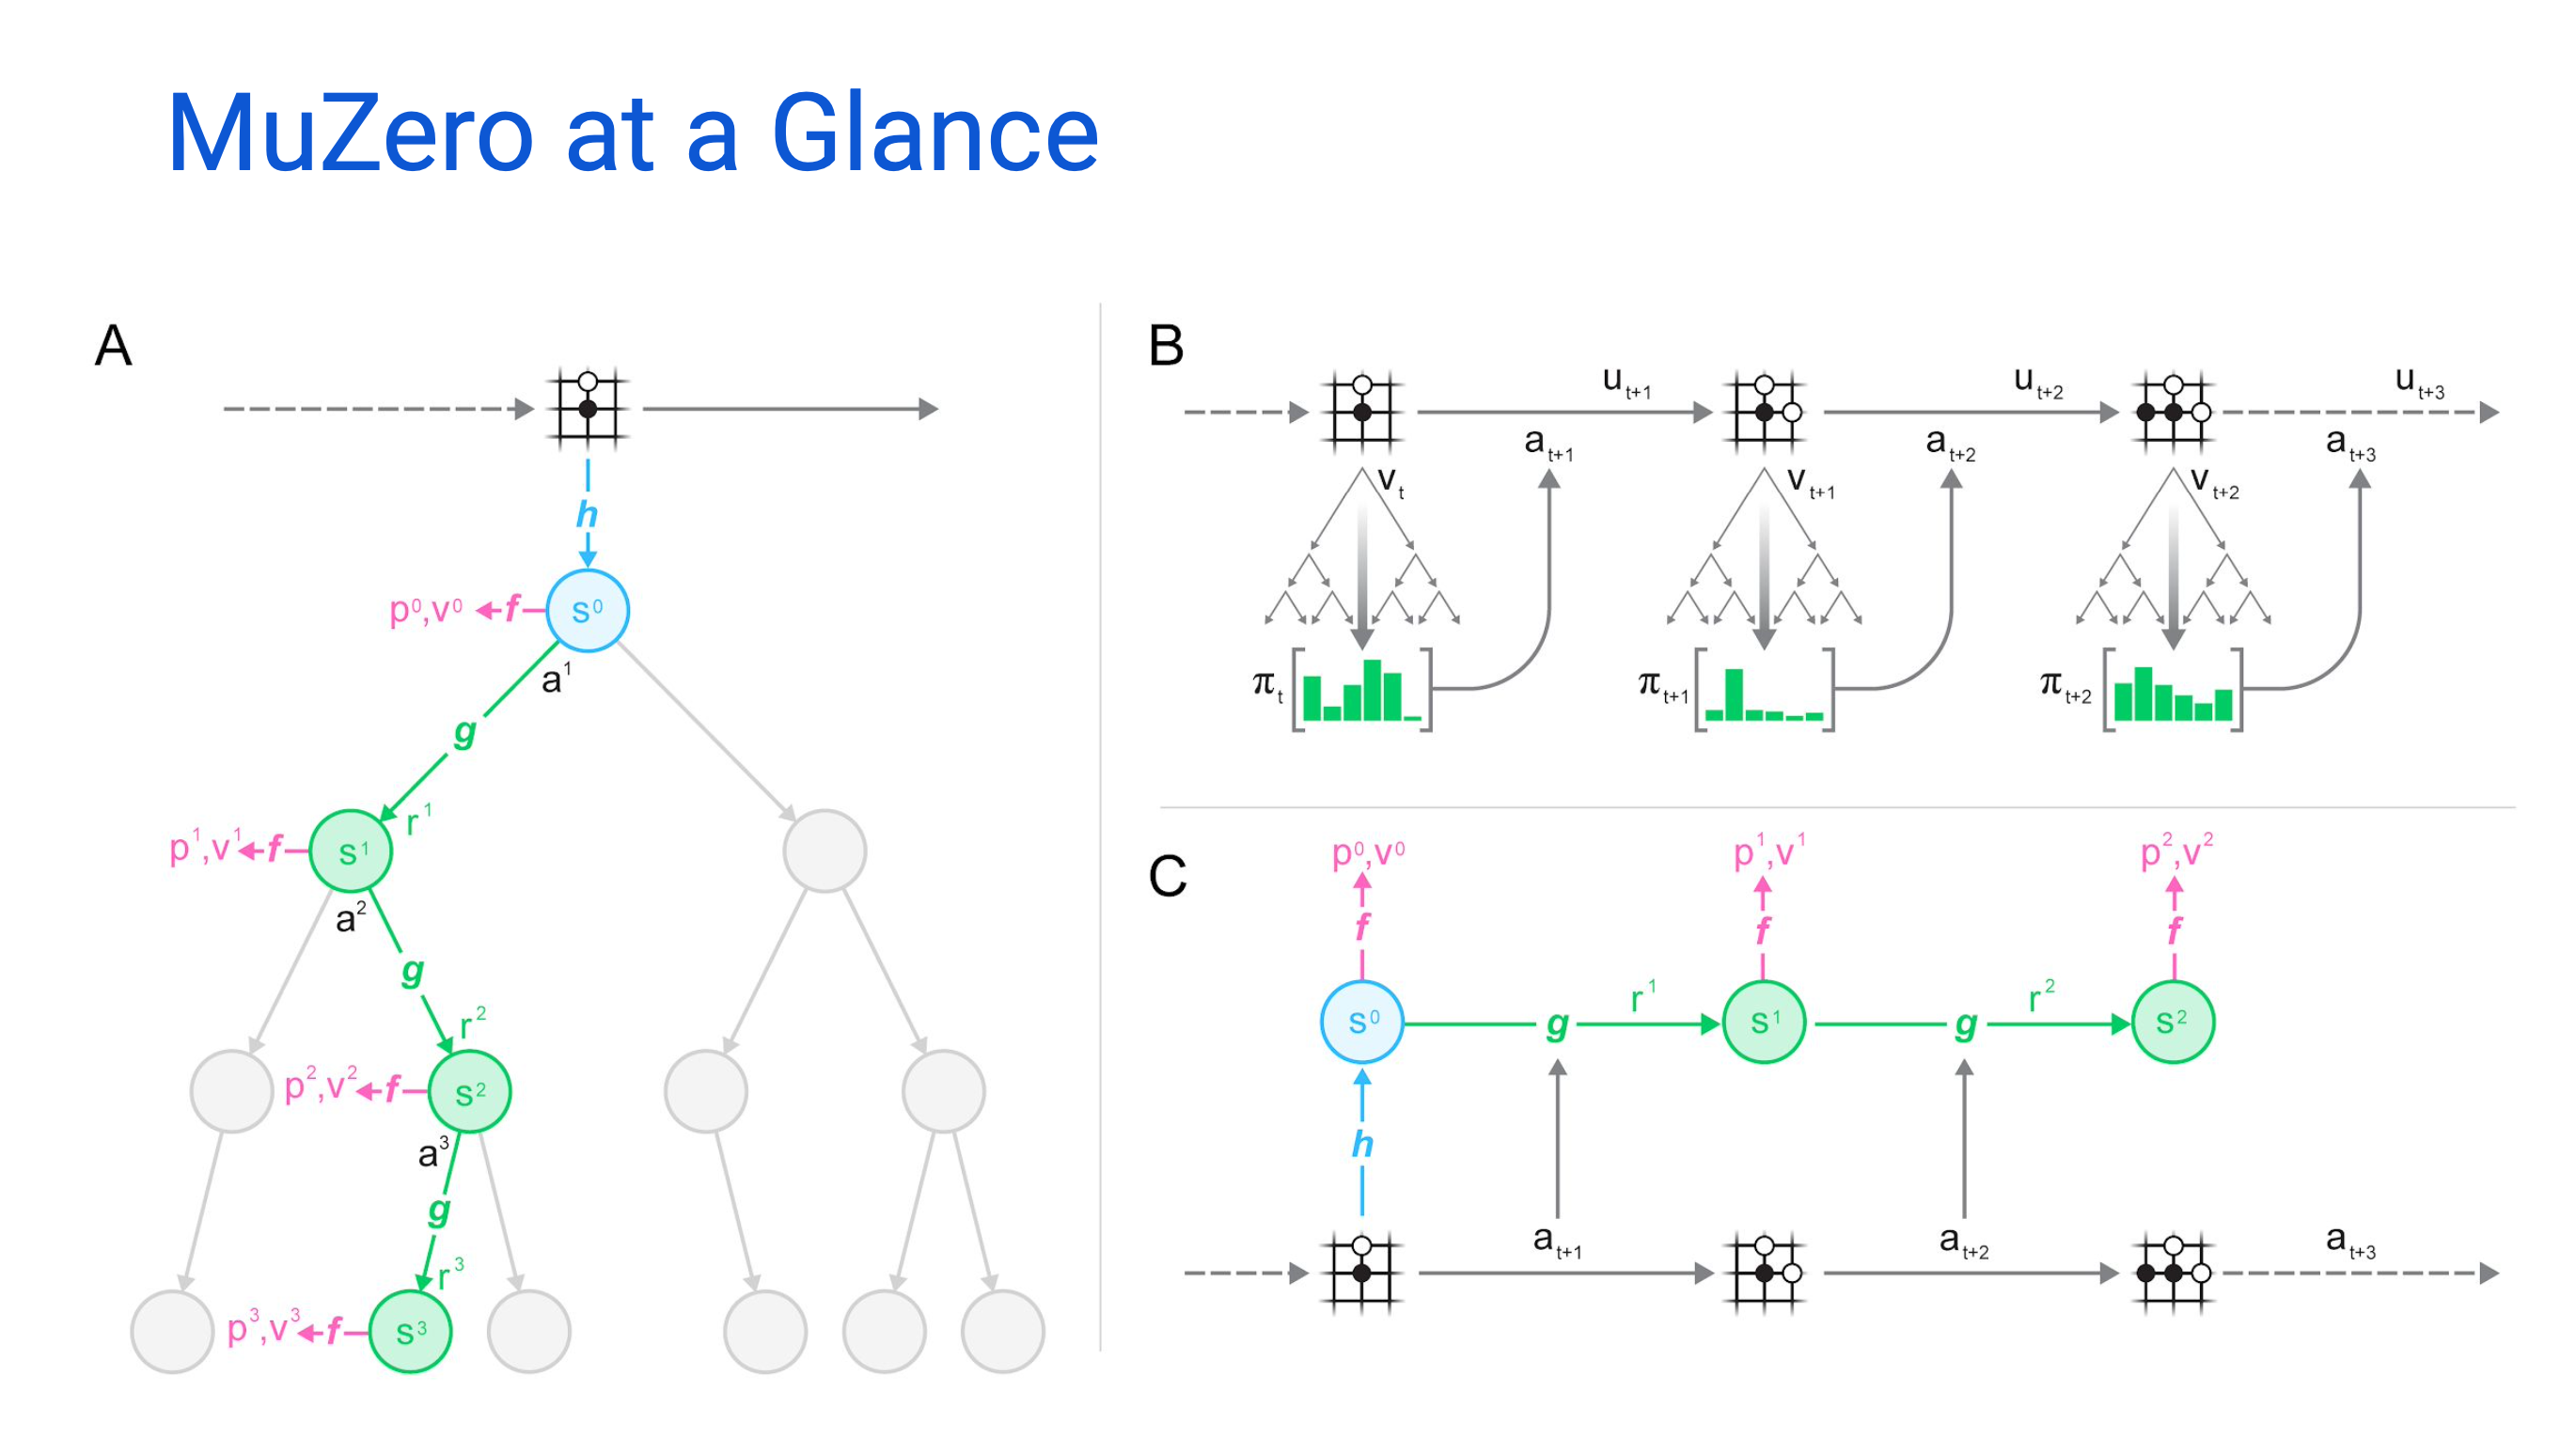
\includegraphics[width=400px,height=200px]{images/muzero_planning.png}
       \caption{MuZero at a Glance}
       \label{fig:my_label}
\end{figure}


\section{MCTS as regularized policy optimization}

A paper by Jean-Bastien Grill and colleagues #TODO [Citation] proposed to show in rigorous detail the theoretical understanding for what AlphaZero actually is. They show that AlphaZero and similar MCTS based algorithms are really approximations to a regularized policy optimization problem. They also show that it is possible to find the exact solution and use that as a replacement for AlphaZero and obtain better results. I think that this was a fantastic paper and will really help you understand AlphaZero if you take the time to go through it. Lets look at some of the highlights of the paper. 

First it is necessary to understand what \textbf{policy optimization} is. This is an approach to solving RL type problems by directly maximizing reward by looking at the gradient of your loss function w.r.t the parameters of your policy network. So the optimal policy is obtained by incrementally improving the policy network directly. The regularized version of this concept is discussed in the current paper. Here is the maximization problem that is trying to be solved.

\begin{equation}
    \pi_{\theta^{'}} \overset{\triangle}{=} \underset{y \epsilon S}{arg \ max} Q_{\pi_{\theta}}^{T}\y - R(y,\pi_{\theta})
\end{equation}

Q is the same Q function that we have seen in AlphaZero. The subscript just means that it is a value estimate w.r.t a certain policy. \textbf{y} is a vector that represents the action distribution that we are looking for to maximize the equation. $R(y,\pi_\theta)$ is a regularization term. Their main claim in this paper is that the selection criterion use by AlphaZero "can be interpreted as approximating the solution to a regularized policy-optimization objective". Some notation will be needed to understand the core concepts of the paper. First they define a multiplier that is used to help simplify some expressions. 

\begin{equation}
    \lambda_{N} (s) \overset{\triangle}{=} c * \frac{\sqrt{\sum_{b}n_{b}}}{|\mathbf{A}| + \sum_{b}n_{b}}
\end{equation}

Most of these terms we have seen alread. $| \mathbf{A} |$ is the number of possible actions in the given domain and $n_{b}$ is the number of times a particular node has been visited. $c$ is the $puct$ constant. This allows them to rewrite the MCTS select criterion. 

\begin{equation}
    a^{*} \overset{\triangle}{=} arg \ max [\textbf{q} + \lambda_{N} \frac{\pi_{\theta}}{\hat{\pi}}]
\end{equation}

Here $\textbf{q} = Q(s,a)$ and $ \pi_{\theta} = \pi_{\theta}(a | s)$ the policy distribution from our network and $\hat{\pi}$ is the policy distribution given by MCTS. They show that $\hat{\pi}$ is an approximation to a solution (${\bar{\pi}}$) of a regularized policy optimization problem.

\begin{equation}
    \bar{\pi} \overset{\triangle}{=} \underset{y \epsilon S}{arg \ max} \ \textbf{q}^{T}\y - \lambda_{N}KL(\pi_{\theta},y)
\end{equation}

Here the regularization term is KL-divergence and is in reverse of how it is normally written. They show that $\hat{\pi}$ actually tracks $\bar{\pi}$. They also show how the MCTS UCT that we looked at early in this paper is actually approximating a similar $\bar{\pi}$ but with a different regularization term. They then describe why just calculating $\bar{\pi}$ directly is preferable. Since $\bar{\pi}$ can be substituted in place of $\hat{\pi}$ you can just swap out one for the other in any place that it is used. In AlphaZero $\hat{\pi}$ is used in three places. It is used in selecting actions, during search and also when training the network. 

To demonstrate the applicability of their approach they ran a series of experiments using MuZero as a baseline. The first figure below helps demonstrate that MuZero is indeed approximating their algorithm and also the large impact that the number of simulations has on performance for MuZero. "All" in this figure stands for the fact that they swapped in $\bar{\pi}$ for each one of the three steps that were mentioned above. We can see that especially for a small number of simulations "All" vastly outperforms MuZero but they converge to equal performance as the simuations are increased. 

\begin{figure}[H]
       \centering
       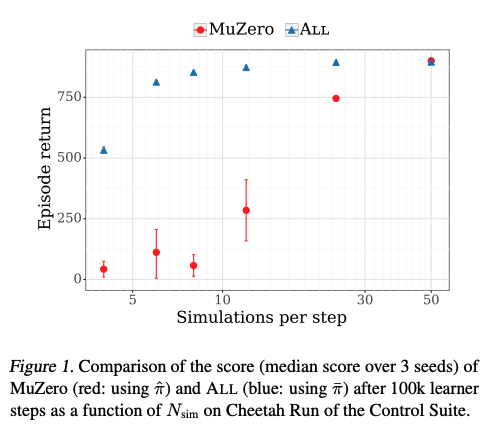
\includegraphics[width=400px,height=200px]{experiments/mcts_reg_figure_1.png}
       \label{fig:my_label}
\end{figure}

They performed experiments a number of Atari games and seem to demonstrate quite definitively the performance gains achieved using their method. This paper is quite impressive and well worth your time to go and read it if you want to have a deeper understanding of AlphaZero.  


\begin{figure}[H]
       \centering
       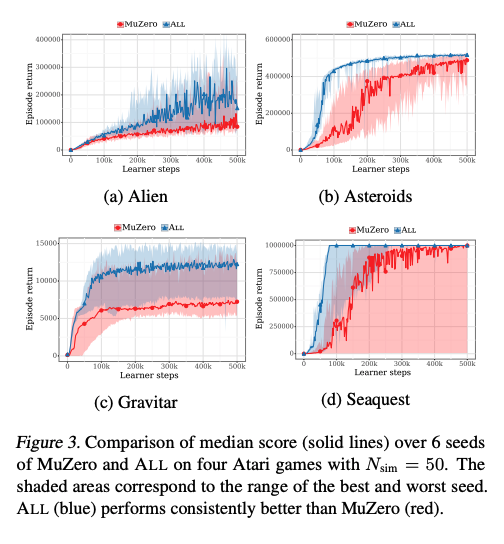
\includegraphics[width=400px,height=200px]{experiments/mcts_reg_figure_3.png}
       \label{fig:my_label}
\end{figure}

\section{Other work and applications AlphaZero}

I will just point the reader at a few papers that extend ALphaZero or use it in a novel way. There is many more I am sure at this point as the literature continues to expand at a rapid pace in this area. 

\begin{itemize}
    \item AlphaZero is intended to work in domains in which the action space is discrete. Extending the work to continous actions space would greatly help in being able to use it in "real" world applications such as robotics.
    \textbf{A0C: Alpha Zero in Continuous Action Space}
    \cite{aocalphazero}
    
    \item \textbf{Improved protein structure prediction using potentials from deep learning}
    \cite{alphafold}
    
    \item \textbf{TOWARDS “ALPHA CHEM”: CHEMICAL SYNTHESIS PLANNING WITH TREE SEARCH AND
    DEEP NEURAL NETWORK POLICIES}
    \cite{alphachem}
    
    \item Optimizing quantum dynamics
    \textbf{Dalgaard, Mogens, et al. "Global optimization of quantum dynamics with AlphaZero deep exploration." npj Quantum Information 6.1 (2020).}
    \cite{alphaquantum} 
    
\end{itemize}



\chapter{Conclusion}

In this paper we have looked at the AlphaGo family of algorithms in the hopes of shedding some light on how the internals work. We have taken the perspective of looking at 2 player zero sum games and how they have historically been solved. We then showed how AlpahGo fits into this history. We discussed a bit about what goes into actually building out your own version of the program. Using our own version we looked at a number of experiments that helped us understand how the different parameters of the algorithm affect overall performance. The AlphaZero algorithm is quite elegant but it requires a tremendous amount of tuning. This tuning cost is prohibitively costly in larger domains if you are on a limited budget. That being said the algorithm has proven to be very successful in the game of Go and in other domain. In concluding this paper I would like to highlight a few advances since AlphaZero that are worth noting. I hope that these will givc the reader a good idea of where to go next if they are interested in pursuing this topic further.


\listoffigures

\printbibliography

\end{document}
